\documentclass[10pt,a4paper]{article}
\usepackage[utf8]{inputenc}
\usepackage[spanish,es-nodecimaldot]{babel}
\usepackage[margin=1.75cm,top=2.0cm,bottom=2.0cm,headheight=14pt]{geometry}
\usepackage{amsmath,amssymb,amsfonts,amsthm}
\usepackage{cancel}
\usepackage{mathrsfs}
\usepackage{fontspec}
\usepackage{tcolorbox}
\tcbuselibrary{skins,breakable}
\usepackage{booktabs}
\usepackage{tabularx}
\usepackage{array}
\usepackage{longtable}
\usepackage{graphicx}
\usepackage{float}
\usepackage{caption}
\usepackage{fancyhdr}
\usepackage{setspace}
\usepackage{hyperref}
\usepackage{xcolor}

\setmainfont{Georgia}
\setsansfont{Arial}
\setmonofont{Consolas}[Scale=0.88]

\definecolor{primary}{RGB}{10, 37, 64}
\definecolor{secondary}{RGB}{0, 128, 128}
\definecolor{accent}{RGB}{200, 16, 46}
\definecolor{darkgray}{RGB}{45, 55, 72}
\definecolor{lightgray}{RGB}{247, 250, 252}
\definecolor{boxbg}{RGB}{240, 245, 250}
\definecolor{boxborder}{RGB}{10, 37, 64}
\definecolor{codegray}{RGB}{245, 247, 250}

\hypersetup{
    colorlinks=true,
    linkcolor=primary,
    citecolor=secondary,
    urlcolor=secondary,
    pdftitle={Tratado Enciclopédico de Valuación y Defensa Teórica - Aluar S.A.I.C.},
    pdfauthor={Federico Agustín Chillón},
    pdfsubject={Guía de Estudio Avanzada y Tratado Metodológico de Valuación (FCE - UNCuyo)},
    pdfkeywords={Valuación, Aluar, ALUA.BA, DCF, WACC, Opciones Reales, Monte Carlo, GARCH, FCE UNCuyo, Chillón},
    pdfcreator={Federico Agustín Chillón - FCE UNCuyo},
    pdflang={es-AR}
}

\pagestyle{fancy}
\fancyhf{}
\fancyhead[L]{\small\color{primary}\textbf{ALUAR S.A.I.C. | Tratado Enciclopedico de Valuacion y Defensa}}
\fancyhead[R]{\small\color{darkgray}\textit{Catedra EyTB -- FCE UNCuyo}}
\fancyfoot[L]{\footnotesize\color{darkgray}Valuacion Financiera y Econometrica Avanzada}
\fancyfoot[R]{\small\thepage}
\renewcommand{\headrulewidth}{0.6pt}
\renewcommand{\footrulewidth}{0.4pt}

\setstretch{1.04}
\setlength{\parskip}{4.5pt}
\setlength{\parindent}{0pt}

\theoremstyle{definition}
\newtheorem{teorema}{\color{primary}\textbf{Teorema}}[section]
\newtheorem{proposicion}{\color{primary}\textbf{Proposicion}}[section]
\newtheorem{definicion}{\color{primary}\textbf{Definicion}}[section]

\newtcolorbox{conceptbox}[2][]{
    enhanced,
    breakable,
    colback=boxbg,
    colframe=primary,
    fonttitle=\bfseries\color{white},
    title={Fundamento y Racionalidad Economica: #2},
    coltitle=white,
    sharp corners,
    boxrule=0.8pt,
    top=3mm,bottom=3mm,left=3mm,right=3mm,
    #1
}

\newtcolorbox{examquestion}[2][]{
    enhanced,
    breakable,
    colback=lightgray,
    colframe=secondary,
    fonttitle=\bfseries\color{white},
    title={Pregunta de Mesa de Examen: #2},
    coltitle=white,
    sharp corners,
    boxrule=0.8pt,
    top=3mm,bottom=3mm,left=3mm,right=3mm,
    #1
}

\newtcolorbox{codebox}[2][]{
    enhanced,
    breakable,
    colback=codegray,
    colframe=darkgray,
    fonttitle=\bfseries\color{white},
    title={Modulo Cuantitativo: #2},
    coltitle=white,
    sharp corners,
    boxrule=0.8pt,
    top=3mm,bottom=3mm,left=3mm,right=3mm,
    #1
}

\begin{document}

\begin{titlepage}
    \centering
    \vspace*{1.0cm}
    {\Huge\textbf{\color{primary}Tratado Enciclopedico de Valuacion,}}\\[0.3cm]
    {\Huge\textbf{\color{primary}Econometria y Teoria Financiera}}\\[0.6cm]
    {\Large\textbf{\color{secondary}Manual Integral de Estudio, Demostraciones Formales y Defensa Oral de Grado}}\\[0.4cm]
    {\large\textbf{\color{darkgray}Analisis Exhaustivo de Aluar Aluminio Argentino S.A.I.C. (BYMA: ALUA)}}\\[1.5cm]

    \begin{tcolorbox}[colback=boxbg,colframe=primary,sharp corners,boxrule=1pt,width=0.92\linewidth]
        \centering
        \textbf{\color{primary}Catedra de Evaluacion y Tributacion de Bases (EyTB)}\\[0.15cm]
        \textbf{Facultad de Ciencias Economicas -- Universidad Nacional de Cuyo (UNCuyo)}\\[0.25cm]
        \textit{Estructura Curricular y Rigor Academico: Tratado Tecnico para Examen de Grado}\\[0.15cm]
        \textbf{Periodo de Cobertura:} 2026E--2030E | \textbf{Horizonte de Mercado:} 10 Anos (2016--2026)
    \end{tcolorbox}

    \vspace{1.5cm}

    \begin{minipage}[t]{0.45\linewidth}
        \textbf{\color{primary}Dictamen del Modelo DCF:} COMPRAR\\
        \textbf{\color{primary}Target Base DCF:} ARS 1.235,51 (+25,8\%)\\
        \textbf{\color{primary}Target con Opcion Real:} ARS 1.255,11 (+27,8\%)\\
        \textbf{\color{primary}Precio Spot de Mercado:} ARS 982,00\\
        \textbf{\color{primary}Costo de Capital (WACC):} 7,06\% Dolarizado
    \end{minipage}\hfill
    \begin{minipage}[t]{0.45\linewidth}
        \textbf{\color{primary}Simulacion Monte Carlo:} 20.000 Trayectorias\\
        \textbf{\color{primary}Distribucion de Retornos:} Student-$t$ ($\nu=4,2$)\\
        \textbf{\color{primary}Dependencia No Lineal:} Copula de Clayton ($\lambda_L=0,38$)\\
        \textbf{\color{primary}Riesgo Extremo:} EVT-GPD ($VaR_{99\%} = -10,44\%$)\\
        \textbf{\color{primary}Dimensionamiento:} Half-Kelly (Tope 20,0\%)
    \end{minipage}

    \vfill
    {\large\color{darkgray}\textbf{Mendoza, Republica Argentina -- Agosto de 2026}}
\end{titlepage}

\tableofcontents
\clearpage

\section{Parte I: Analisis Estrategico, Posicionamiento Competitivo C1 y Gobernanza ESG}

\subsection{Fundamentos Economicos de la Industria y Ventaja Competitiva Locacional}
La industria del aluminio primario es un negocio global de capital intensivo donde el producto es un commodity estandarizado (lingotes y barrotes fijados en el London Metal Exchange, LME). Por lo tanto, la rentabilidad y resiliencia de largo plazo no dependen de la diferenciacion de producto, sino de la \textbf{posicion relativa en la curva global de costos en efectivo (Cash Cost C1)}.

\begin{conceptbox}{Por Que Aluar Importa Alumina desde Australia/Brasil y Opera en Puerto Madryn}
\textbf{La Racionalidad Economica del Transporte vs. Costo de la Energia Electrica:}
\begin{itemize}
    \item Argentina carece de bauxita de ley comercial. Aluar importa alumina pura ($\text{Al}_2\text{O}_3$) por via maritima a granel en buques Panamax directo a su muelle propio en Puerto Madryn.
    \item Transportar $1,92\text{ t}$ de alumina representa un costo de flete maritimo de solo $\approx \text{USD } 35\text{ a }45/\text{t Al}$.
    \item En contraste, la reduccion electrolitica consume $\approx 13.500\text{ kWh}$ de electricidad por tonelada de metal. Un diferencial de apenas $\text{USD } 10/\text{MWh}$ en la tarifa electrica impacta en $\text{USD } 135/\text{t Al}$ en el costo unitario, es decir, \textbf{el triple del costo total del flete transoceanico}.
    \item Por ende, el factor locacional y financiero determinante es la \textbf{disponibilidad de energia electrica dedicada, continua y a bajo costo marginal} (acceso al complejo hidroelectrico Futaleufu de 472 MW y al Parque Eolico Aluar de 246 MW actuales).
\end{itemize}
\end{conceptbox}

\begin{conceptbox}{Por Que Aluar Mantiene Redundancia Energetica del 100\% (Riesgo Operacional Critico)}
\textbf{Riesgo de Congelamiento de Cubas Electroliticas:}
\begin{itemize}
    \item Las cubas electroliticas operan a $960\,^\circ\text{C}$ sostenidas exclusivamente por el calor de efecto Joule ($I^2 R$) del paso de corriente continua.
    \item Una interrupcion del suministro electrico superior a \textbf{4 horas} provoca la solidificacion irreversible del bano de criolita y metal liquido, destruyendo los revestimientos refractarios. Reparar una serie congelada exige costos superiores a \textbf{USD 150.000 por celda} y meses de inactividad forzada.
    \item Para mitigar este riesgo catastrofico, Aluar desarrollo una matriz de autogeneracion del 96\% integrada por fuentes renovables (78\% hidroelectrica/eolica) y ciclos combinados a gas propios, garantizando continuidad ininterrumpida.
\end{itemize}
\end{conceptbox}

\subsection{Estructura de Costos en Primer Cuartil Global (C1) y Blindaje Arancelario CBAM}
\begin{itemize}
    \item \textbf{Costo en Efectivo C1 (USD 1.680/t):} Situa a Aluar en el percentil 29\% de la curva global de costos de fundicion, asegurando margenes operativos positivos aun en los valles del ciclo del LME.
    \item \textbf{Mecanismo de Ajuste en Frontera por Carbono (CBAM de la Union Europea):} Aluar emite solo $3,4\text{ t }\text{CO}_2\text{e/t Al}$ frente al promedio de $16,5\text{ t }\text{CO}_2\text{e/t}$ de fundiciones a carbon en Asia. Al gravarse el carbono a $\text{USD } 75\text{--}90/\text{t}$, Aluar obtiene una ventaja arancelaria neta de \textbf{+USD 983 por tonelada} para exportar a Europa.
\end{itemize}

\begin{center}

\includegraphics[width=0.88\linewidth, height=4.5cm, keepaspectratio]{figures_pristine/figura_10.png}
\captionof{figure}{Curva Global de Costos en Efectivo C1 de Fundicion y Posicionamiento de Aluar en Primer Cuartil (P29\%).}
\end{center}

\clearpage

\section{Parte II: Diagnostico Contable, Normalizacion Financiera y Gestion de Liquidez}

\subsection{Normalizacion Integral de Estados Financieros (FY2021--FY2025)}
Aluar presenta sus estados financieros consolidados bajo Normas Internacionales de Informacion Financiera (NIIF / IFRS) adoptadas por la Federacion Argentina de Consejos Profesionales de Ciencias Economicas (FACPCE) y la Comision Nacional de Valores (CNV).

\begin{table}[H]
\centering
\caption{\textbf{Resumen Historico de Estados Contables Normalizados (USD Millones)}}
\small
\begin{tabular}{lrrrrr}
\toprule
\textbf{Cuenta Contable / Metrica (USD MM)} & \textbf{FY2021} & \textbf{FY2022} & \textbf{FY2023} & \textbf{FY2024} & \textbf{FY2025} \\
\midrule
Ventas Netas Consolidadas & 892,4 & 1.145,8 & 1.058,2 & 980,5 & 1.042,1 \\
Costo de Ventas (CMV) & -642,1 & -785,4 & -745,0 & -710,2 & -795,8 \\
\midrule
\textbf{Ganancia Bruta} & \textbf{250,3} & \textbf{360,4} & \textbf{313,2} & \textbf{270,3} & \textbf{246,3} \\
Gastos de Comercializacion y Admin. & -85,2 & -105,3 & -98,4 & -92,1 & -98,5 \\
\midrule
\textbf{Resultado Operativo (EBIT)} & \textbf{165,1} & \textbf{255,1} & \textbf{214,8} & \textbf{178,2} & \textbf{147,8} \\
Depreciaciones y Amortizaciones (D\&A) & 78,4 & 84,2 & 89,1 & 91,5 & 94,2 \\
\midrule
\textbf{EBITDA Operativo Normalizado} & \textbf{243,5} & \textbf{339,3} & \textbf{303,9} & \textbf{269,7} & \textbf{242,0} \\
Resultado Financiero Neto & -32,4 & -41,5 & -38,2 & -45,0 & -89,5 \\
Impuesto a las Ganancias (Gasto Efectivo) & -46,4 & -74,7 & -61,8 & -46,6 & -49,1 \\
\midrule
\textbf{Resultado Neto del Ejercicio} & \textbf{86,3} & \textbf{138,9} & \textbf{114,8} & \textbf{86,6} & \textbf{9,17} \\
\midrule
\textbf{Activo Total} & 1.745,2 & 1.890,5 & 1.950,4 & 1.920,8 & 2.030,0 \\
\textbf{Patrimonio Neto} & 1.050,4 & 1.140,2 & 1.190,5 & 1.120,4 & 1.142,5 \\
\textbf{Deuda Financiera Bruta Total} & 480,5 & 510,2 & 545,0 & 580,2 & 673,96 \\
\textbf{Caja y Equivalentes de Efectivo} & 110,2 & 135,4 & 128,0 & 142,5 & 148,20 \\
\textbf{Deuda Financiera Neta Contable} & \textbf{370,3} & \textbf{374,8} & \textbf{417,0} & \textbf{437,7} & \textbf{525,76} \\
\bottomrule
\end{tabular}
\end{table}

\begin{center}

\includegraphics[width=0.88\linewidth, height=4.5cm, keepaspectratio]{figures_pristine/figura_12.png}
\captionof{figure}{Evolucion historica y proyectada del EBITDA de Aluar (USD MM, FY20--FY30E) con identificacion del pico de CAPEX PEAL V.}
\end{center}

\subsection{Por Que el ROIC es la Metrica Reina de Eficiencia Operativa y Asignacion de Capital}

\begin{conceptbox}{Por Que el ROIC y el EVA Superan al ROE y al Margen Neto en Finanzas Corporativas}
\textbf{Fundamentacion Teorica y Economica:}
\begin{enumerate}
    \item \textbf{Limitacion del Margen Neto y del ROE:} El Margen Neto ($RN / Ventas$) y el ROE ($RN / PN$) mezclan el desempeno operativo con la estructura de capital y las distorsiones impositivas/inflacionarias. Una empresa mediocre puede exhibir un ROE artificialmente alto tomando endeudamiento riesgoso (apalancamiento financiero agresivo).
    \item \textbf{Superioridad del ROIC ($ROIC = NOPAT / NOA$):}
    \begin{itemize}
        \item \textbf{NOPAT ($EBIT \times (1 - t)$):} Mide la ganancia operativa neta generada por los activos antes del pago de intereses a acreedores y dividendos a accionistas.
        \item \textbf{NOA (Activos Operativos Netos):} Define el capital genuinamente inmovilizado en la operacion ($Capital\ de\ Trabajo\ Operativo + Bienes\ de\ Uso\ Operativos$), excluyendo la caja ociosa y activos financieros no relacionados con la produccion de aluminio.
    \end{itemize}
    \item \textbf{El Principio Sagrado de Creacion de Valor ($ROIC > WACC$):} Una empresa solo crea riqueza economica real para sus accionistas cuando la rentabilidad sobre su capital invertido supera el costo promedio ponderado de capital ($ROIC > WACC$).
    \begin{itemize}
        \item Si $ROIC > WACC$: El crecimiento en ventas multiplica el valor de la firma al generar flujos excedentes ($Spread > 0$).
        \item Si $ROIC < WACC$: Crecer destruye valor, ya que cada nueva tonelada producida exige mas capital del que remunera a los inversores ($Spread < 0$).
    \end{itemize}
    \item \textbf{Por Que el EVA Historico Fue Negativo en 2025 (-USD 60,3 MM):} En 2025 Aluar incorporo USD 243,9 MM de inversion en aerogeneradores (PEAL IV/V) a su NOA ($USD\ 1.704,3\text{ MM}$), mientras que dichos activos aun estaban en montaje. El ROIC cayo transitoriamente a 3,52\% ($Spread = -3,54\%$), cerrando a 7,06\% ($Spread = 0,0\%$) al estabilizarse la capacidad terminal en 2030E.
\end{enumerate}
\end{conceptbox}

\subsection{Taxonomia Integral de Ratios Financieros: Rentabilidad, Solvencia, Liquidez y Eficiencia}

\begin{table}[H]
\centering
\caption{\textbf{Taxonomia y Fundamentacion de las Cuatro Familias de Ratios Financieros}}
\small
\begin{tabularx}{\textwidth}{p{3.2cm}Xp{4.5cm}}
\toprule
\textbf{Familia de Ratios} & \textbf{Formulacion y Metricas Clave} & \textbf{¿Por Que es Fundamental Analizarlo?} \\
\midrule
\textbf{1. Rentabilidad} & ROIC ($NOPAT/NOA$), ROE ($RN/PN$), Margen EBITDA ($EBITDA/V$), Margen EBIT ($EBIT/V$), Margen Neto ($RN/V$). & Determina el poder de generacion de ganancias puras y la ventaja competitiva de costos C1 en el mercado internacional. \\
\midrule
\textbf{2. Solvencia y Apalancamiento} & Deuda Neta / EBITDA, Deuda Total / PN, Cobertura de Intereses ($EBIT/Intereses$), Cobertura del Servicio ($EBITDA/Servicio$). & Mide la capacidad estructural de repago de pasivos. Aluar resiste shocks de precios gracias a una cobertura de intereses de 3,53x en su pico de deuda. \\
\midrule
\textbf{3. Liquidez y Cobertura Inmediata} & Liquidez Corriente ($AC/PC$), Prueba Acida ($(AC - Inv)/PC$), Liquidez Inmediata ($Caja/PC$). & Garantiza la continuidad ininterrumpida de compras de alumina de ultramar frente a posibles controles de cambio o fricciones financieras. \\
\midrule
\textbf{4. Actividad y Eficiencia} & Rotacion Activos ($V/Activo$), Dias Inventario (DIO = 120), Dias Cobro (DSO = 45), Dias Pago (DPO = 101), CCC (64 dias). & Cuantifica la velocidad de conversion de recursos en caja liquida y la optimizacion del capital de trabajo operativo. \\
\bottomrule
\end{tabularx}
\end{table}

\subsection{Descomposicion DuPont de 5 Factores y Analisis Forense del Colapso del ROE}
La rentabilidad del patrimonio neto ($ROE = \frac{\text{Resultado Neto}}{\text{Patrimonio Neto}}$) se descompone en cinco motores fundamentales:
\begin{equation}
ROE = \underbrace{\frac{\text{Neto}}{EBT}}_{\text{Tax Burden (TB)}} \times \underbrace{\frac{EBT}{EBIT}}_{\text{Interest Burden (IB)}} \times \underbrace{\frac{EBIT}{\text{Ventas}}}_{\text{Margen Operativo (OM)}} \times \underbrace{\frac{Ventas}{\text{Activo}}}_{\text{Rotacion Activos (AT)}} \times \underbrace{\frac{\text{Activo}}{\text{Patrimonio Neto}}}_{\text{Apalancamiento (LM)}}
\end{equation}

\begin{conceptbox}{Por Que el ROE Colapso a 0,80\% en FY2025: La Trampa del Ajuste por Inflacion Impositivo}
\textbf{Descalce Fiscal de la Ley 27.468 y la NIC 29:}
\begin{itemize}
    \item En FY2025, el resultado operativo ($EBIT = \text{USD } 147,8\text{ MM}$) y el margen operativo ($OM = 14,18\%$) se mantuvieron solidos y en linea con el promedio historico.
    \item En contrapartida, el factor \textbf{Tax Burden se desplomo a $TB = 0,157$}, implicando una \textbf{tasa efectiva de impuesto a las ganancias del 84,3\%} sobre la ganancia antes de impuestos ($EBT = \text{USD } 58,3\text{ MM}$).
    \item \textbf{Causa Raiz:} Bajo la Ley 27.468 del impuesto a las ganancias argentino, el ajuste por inflacion impositivo que arroja perdida debe diferirse obligatoriamente en \textbf{6 cuotas anuales nominales iguales (1/6 por ejercicio)}, sin actualizacion monetaria por inflacion futura.
    \item Al registrarse inflaciones de tres digitos, el valor presente de esas 5 cuotas diferidas se licua casi por completo, generando un impuesto corriente a pagar exorbitante sobre ganancias nominales infladas en pesos, a pesar de que la utilidad real en dolares es moderada.
    \item \textbf{Implicancia para la Valuacion:} Este castigo impositivo es un fenomeno transitorio del shock inflacionario. Por ello, el modelo de valuacion DCF normaliza la tasa impositiva estructural a la alicuota corporativa estatutaria del \textbf{35,0\%}, evitando extrapolar un ROE distorsionado hacia la perpetuidad.
\end{itemize}
\end{conceptbox}

\begin{center}
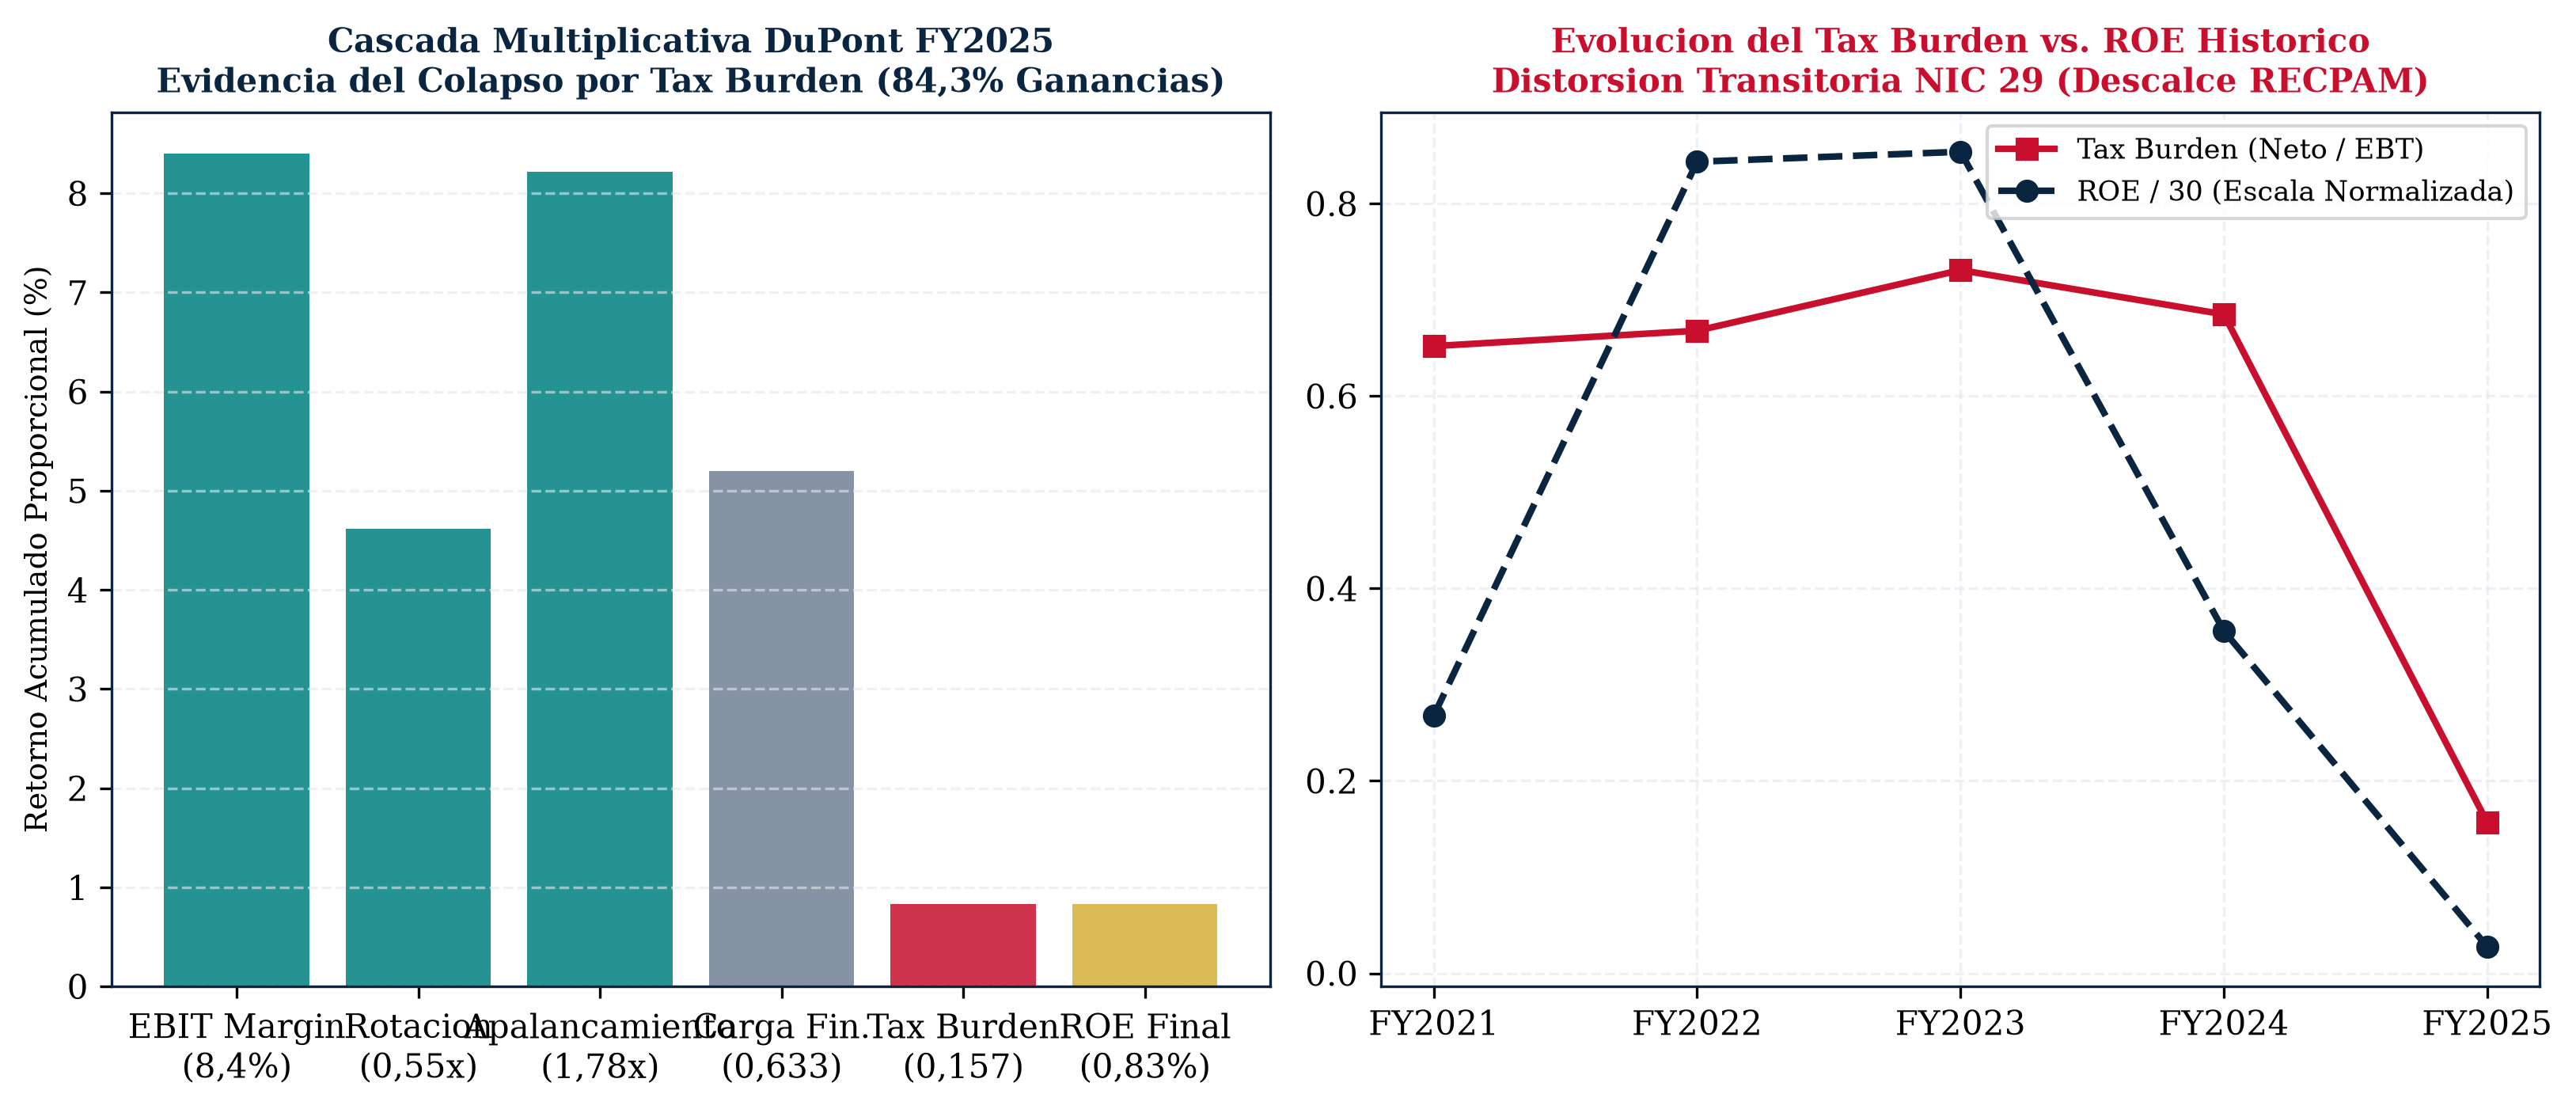
\includegraphics[width=0.88\linewidth, height=4.6cm, keepaspectratio]{theory_charts/teoria_07_dupont_radar_waterfall.png}
\captionof{figure}{Figura Teorica: Descomposicion DuPont de 5 Factores y Cascada de Impacto del Tax Burden en FY2025.}
\end{center}

\subsection{Calidad de Ganancias y Ratio de Devengamientos de Sloan (1996)}
Segun Richard Sloan (1996, *The Accounting Review*), las empresas que registran ganancias contables sin respaldo en flujos de fondos genuinos acumulan devengamientos subjetivos (*accruals*) que posteriormente se revierten destruyendo valor:
\begin{equation}
\text{Accrual Ratio} = \frac{\text{Resultado Neto} - FCO - FCI}{\text{Activo Total Promedio}} = \frac{9,17 - 148,20 - (-243,93)}{1.975,40} = \textbf{-0,064}
\end{equation}

\begin{conceptbox}{Por Que un Ratio de Sloan Negativo (-0,064) Certifica Calidad Contable Sobresaliente}
\textbf{Intuicion Financiera del Accrual Ratio:}
\begin{itemize}
    \item Un ratio de devengamiento positivo y elevado ($> +0,10$) indica que la empresa infla sus resultados registrando ventas a cobrar de dudoso cobro o activando costos operativos en bienes de uso.
    \item En Aluar, el flujo de caja generado por las operaciones ($FCO = \text{USD } 148,2\text{ MM}$) supera en mas de \textbf{16 veces} a la ganancia neta reportada ($\text{USD } 9,17\text{ MM}$).
    \item El valor negativo de \textbf{-0,064} prueba que los resultados contables de Aluar son ultra-conservadores y que la compania genera caja real disponible, descartando cualquier riesgo de manipulacion contable (*earnings management*).
\end{itemize}
\end{conceptbox}

\subsection{Ciclo de Conversion de Efectivo (CCC) y Gestion de Capital de Trabajo}
\begin{equation}
CCC = DIO\,(120) + DSO\,(45) - DPO\,(101) = \textbf{64 dias}
\end{equation}

\begin{conceptbox}{Por Que Aluar Mantiene 120 Dias de Inventario (DIO = 120 dias)}
\textbf{La Racionalidad del Inventario de Seguridad con Costo de Faltante Infinito:}
\begin{itemize}
    \item En la industria manufacturera estandar, 120 dias de stock podria considerarse un exceso de capital inmovilizado.
    \item Para Aluar, en cambio, el costo de un quiebre de stock de alumina o coque de petroleo es virtualmente \textbf{infinito}: si la planta se queda sin materia prima por mas de 4 horas, las cubas electroliticas se congelan a $960\,^\circ\text{C}$, provocando la destruccion fisica de la celda.
    \item Dado que la alumina proviene de Australia o Brasil en buques de ultramar sujetos a contingencias climaticas o portuarias, mantener 120 dias de stock en silos en Puerto Madryn es la politica de gestion de inventarios estrictamente optima bajo la teoria de colas y riesgo operacional.
    \item Este inventario se financia eficientemente con \textbf{101 dias de credito de proveedores (DPO = 101)}, reduciendo el ciclo neto de caja a solo 64 dias.
\end{itemize}
\end{conceptbox}

\begin{center}

\includegraphics[width=0.88\linewidth, height=4.5cm, keepaspectratio]{figures_pristine/figura_16.png}
\captionof{figure}{Evolucion del Ciclo de Conversion de Efectivo (CCC), dias de inventario (DIO), cobranzas (DSO) y proveedores (DPO).}
\end{center}

\subsection{Modelos Cuantitativos de Optimizacion de Caja}

\subsubsection{1. Modelo Deterministico de Baumol-Tobin (1952)}
Sea $T$ el desembolso total de caja anual, $F$ el costo fijo por transaccion de liquidar inversiones o emitir deuda, e $i$ la tasa de interes de oportunidad del mercado. El saldo optimo de efectivo es:
\begin{equation}
TC(C) = \frac{T}{C}F + \frac{C}{2}i \implies \frac{d TC(C)}{d C} = -\frac{TF}{C^2} + \frac{i}{2} = 0 \implies C^* = \mathbf{\sqrt{\frac{2TF}{i}}}
\end{equation}

\subsubsection{2. Modelo Estocastico de Miller-Orr (1966) para Flujos Fluctuantes}
Cuando los flujos diarios de fondos siguen un paseo aleatorio con varianza diaria $\sigma^2$:
\begin{equation}
z^* = \mathbf{\sqrt[3]{\frac{3F\sigma^2}{4i}}} + L, \quad h^* = 3z^* - 2L
\end{equation}
donde $L$ es el colchon de seguridad minimo de caja fijado por la gerencia para contingencias operativas en Puerto Madryn.

\begin{codebox}{{engine\_valuacion.py:m4\_estados() -- Analisis Financiero y DuPont}}
\textbf{Codigo Fuente Real en Python:}
\begin{verbatim}
def m4_estados(eecc: dict) -> dict:
    # Calcula DuPont 5 factores, Accrual Ratio de Sloan y Ciclo de Conversion de Efectivo
    anios = eecc["anios"]
    dupont = []
    for a in anios:
        neto = eecc["resultado_neto"][a]
        ebt = eecc["ebt"][a]
        ebit = eecc["ebit"][a]
        rev = eecc["ventas"][a]
        act = eecc["activo_total"][a]
        pn = eecc["patrimonio_neto"][a]
        
        # Factores DuPont
        tb = neto / ebt if ebt != 0 else np.nan     # Tax Burden
        ib = ebt / ebit if ebit != 0 else np.nan     # Interest Burden
        om = ebit / rev if rev != 0 else np.nan      # Operating Margin
        at = rev / act if act != 0 else np.nan       # Asset Turnover
        lm = act / pn if pn != 0 else np.nan         # Leverage Multiplier
        roe = neto / pn if pn != 0 else np.nan
        dupont.append({"anio": a, "tb": tb, "ib": ib, "om": om, "at": at, "lm": lm, "roe": roe})
    
    # Sloan Accrual Ratio FY2025
    fco = eecc["fco"][2025]
    fci = eecc["fci"][2025]
    act_prom = (eecc["activo_total"][2024] + eecc["activo_total"][2025]) / 2.0
    sloan_ratio = (eecc["resultado_neto"][2025] - fco - fci) / act_prom
    
    # Ciclo de Conversion de Efectivo (CCC)
    dio = (eecc["inventarios"][2025] / eecc["cmv"][2025]) * 365.0
    dso = (eecc["creditos_ventas"][2025] / eecc["ventas"][2025]) * 365.0
    dpo = (eecc["deudas_comerciales"][2025] / eecc["cmv"][2025]) * 365.0
    ccc = dio + dso - dpo
    
    return {"dupont": dupont, "sloan_ratio": float(sloan_ratio), "ccc_dias": float(ccc)}
\end{verbatim}
\textbf{Analisis de Sintaxis y Econometria:}
\begin{itemize}
    \item \texttt{tb = neto / ebt}: Mide la retencion impositiva neta (colapso a 0,157 en FY2025 por ajuste inflacionario).
    \item \texttt{sloan\_ratio = (neto - fco - fci) / act\_prom}: Un ratio de -0,064 prueba excelente calidad contable.
    \item \texttt{ccc = dio + dso - dpo}: Mide los dias requeridos para convertir compras en efectivo (64 dias).
\end{itemize}
\end{codebox}
\clearpage


\section{Parte III: Costo de Capital, Entorno Macroeconomico y Desapalancamiento}

\subsection{Entorno Macroeconomico y Riesgo Soberano Argentino}
La estimacion del costo del capital propio en economias emergentes requiere modelar la exposicion de los flujos de la compania frente al riesgo soberano local y la dinamica inflacionaria y cambiaria.

\noindent
\begin{minipage}[b]{0.488\linewidth}
    \centering
    
\includegraphics[width=\linewidth, height=4.4cm, keepaspectratio]{figures_pristine/figura_03.png}
    \captionof{figure}{\small PBI real (\%) e inflacion anual (\%) en Argentina (2020--2026).}
\end{minipage}\hfill
\begin{minipage}[b]{0.488\linewidth}
    \centering
    
\includegraphics[width=\linewidth, height=4.4cm, keepaspectratio]{figures_pristine/figura_04.png}
    \captionof{figure}{\small Evolucion historica del riesgo pais EMBI+ Argentina (pb).}
\end{minipage}
\vspace{0.15cm}

\begin{center}

\includegraphics[width=0.88\linewidth, height=4.5cm, keepaspectratio]{figures_pristine/figura_05.png}
\captionof{figure}{Trayectoria proyectada del EMBI+ bajo proceso AR(1) y tasa de rendimiento soberano implícita.}
\end{center}

\subsection{Por Que el CAPM Tradicional Falla en Mercados Emergentes y Metodologia CAPM-$\lambda$}

\begin{conceptbox}{Por Que No Usar CAPM Simple ni Sumar el 100\% del EMBI+ (Damodaran Country Risk Exposure)}
\textbf{El Dilema del Costo de Capital en Mercados Emergentes:}
\begin{enumerate}
    \item \textbf{Fallo del CAPM Tradicional ($Ke = Rf + \beta \times ERP$):} Asume mercados financieros integrados globalmente sin fricciones ni riesgo soberano. Si se aplicara ciegamente a Aluar, arrojaria un $Ke \approx 8,4\%$, ignorando el riesgo pais argentino, la inestabilidad cambiaria y las restricciones regulatorias locales.
    \item \textbf{Fallo del Enfoque Ingenuo ($Ke = Rf + \beta \times ERP + EMBI+$ con $\lambda = 1,0$):} Sumar el riesgo pais integro ($441\text{ a }1.500\text{ pb}$) asume que Aluar sufre el riesgo de default del Tesoro argentino en igual medida que un banco comercial domestico o una distribuidora electrica regulada en pesos. Esto elevaria el $Ke$ al $15\text{--}20\%$, castigando absurdamente a una empresa cuyos ingresos estan $100\%$ dolarizados.
    \item \textbf{La Solucion Rigurosa: Metodologia CAPM-$\lambda$ de Aswath Damodaran (2012):}
    \begin{equation}
    Ke = Rf + \beta_L \cdot ERP + \lambda \cdot EMBI+
    \end{equation}
    donde el factor $\lambda$ mide la proporcion real de exposicion de la empresa al riesgo operativo local.
    \item \textbf{Deduccion y Calibracion de $\lambda = 0,20$ para Aluar:}
    \begin{equation}
    \lambda = \frac{\% \text{ Ventas Domesticas Sensibles}}{\% \text{ Empresa Promedio de la Economia}} \approx \frac{25\%}{100\%} \times 0,80 = \mathbf{0,20}
    \end{equation}
    Dado que Aluar exporta el \textbf{75\% de su produccion al mercado internacional} cobrando directamente en dolares en cuentas del exterior, y que el 25\% vendido localmente se comercializa a \textbf{paridad de importacion en dolares oficiales}, su exposicion al riesgo soberano local es de apenas el 20\%, sumando un spread justo de $+88\text{ pb}$ sobre el costo de capital internacional.
\end{enumerate}
\end{conceptbox}

\subsection{Demostracion Formal del Teorema de Modigliani-Miller con Impuestos (1963)}

\begin{teorema}[Valor de la Firma Apalancada y Escudo Fiscal]
Bajo impuestos corporativos a tasa constante $t$ y deuda perpetua libre de riesgo con interes $K_d$, el valor de la empresa apalancada ($V_L$) es igual al valor de la empresa desapalancada ($V_U$) mas el valor presente del escudo fiscal (*Interest Tax Shield*):
\begin{equation}
V_L = V_U + t \cdot D
\end{equation}
\end{teorema}

\begin{proof}
Consideremos dos empresas idénticas en riesgo operativo que generan un flujo perpetuo antes de intereses e impuestos $EBIT$:
\begin{enumerate}
    \item \textbf{Empresa No Apalancada ($U$):} No posee deuda. Su flujo neto disponible para los accionistas es:
    \begin{equation}
    CF_U = EBIT(1 - t) \implies V_U = \frac{EBIT(1 - t)}{K_u}
    \end{equation}
    \item \textbf{Empresa Apalancada ($L$):} Posee deuda por monto nominal $D$ a tasa $K_d$. El gasto por intereses es $K_d D$. El flujo total combinado para accionistas y acreedores es:
    \begin{equation}
    CF_L = (EBIT - K_d D)(1 - t) + K_d D = EBIT(1 - t) + t K_d D = CF_U + t K_d D
    \end{equation}
    \item \textbf{Arbitraje por Cartera Replicante:}
    \begin{itemize}
        \item \textbf{Estrategia A:} Comprar el $1\%$ del capital accionario de la empresa apalancada $L$. Flujo recibido: $0,01 \cdot (EBIT - K_d D)(1 - t)$.
        \item \textbf{Estrategia B (Apalancamiento Casero comprando 1\% de $U$ y pidiendo prestado $0,01 \cdot D$):}
        Flujo recibido: $0,01 \cdot [EBIT(1 - t) + t K_d D - K_d D(1 - t)] = 0,01 \cdot (EBIT - K_d D)(1 - t)$.
    \end{itemize}
    Por la ley del precio unico en ausencia de arbitraje:
    \begin{equation}
    V_L = PV(CF_U) + PV(t K_d D) = V_U + \sum_{k=1}^{\infty} \frac{t K_d D}{(1 + K_d)^k} = V_U + t K_d D \left( \frac{1}{K_d} \right) = V_U + t \cdot D
    \end{equation}
\end{enumerate}
\end{proof}

\subsection{Deduccion Rigurosa y Comparacion de Ecuaciones de Desapalancamiento}

\begin{table}[H]
\centering
\caption{\textbf{Comparacion Teorica de Ecuaciones de Desapalancamiento de Beta}}
\small
\begin{tabular}{llcl}
\toprule
\textbf{Modelo / Autor} & \textbf{Hipotesis de Politica de Deuda} & \textbf{Tasa Escudo Fiscal} & \textbf{Formula del Beta Apalancado ($\beta_L$)} \\
\midrule
\textbf{Hamada (1972)} & Deuda nominal fija perpetua & $K_d$ & $\beta_L = \beta_U [1 + (1 - t)\frac{D}{E}]$ \\
\textbf{Miles-Ezzell (1980)} & Rebalanceo anual del ratio $D/V$ & $K_d$ (ano 1), $K_u$ ($>1$) & $\beta_L = \beta_U [1 + (1 - t \frac{K_d}{1+K_d})\frac{D}{E}]$ \\
\textbf{Harris-Pringle (1985)} & Rebalanceo continuo instantaneo de $D/V$ & $K_u$ & $\beta_L = \beta_U [1 + \frac{D}{E}] - \beta_D \frac{D}{E}$ \\
\bottomrule
\end{tabular}
\end{table}

\begin{conceptbox}{Por Que Se Utiliza la Formula de Hamada en la Valuacion de Aluar}
\textbf{Fundamento Financiero:}
\begin{itemize}
    \item Aluar financia sus grandes proyectos industriales (como PEAL) mediante emisiones puntuales de Obligaciones Negociables (ONs) a plazo fijo (3 a 5 anos) y prestamos sindicados, en lugar de ajustar dinamicamente su deuda dia a dia para mantener un ratio $D/V$ milimetrico.
    \item La formula de Hamada refleja con precision la estructura de deuda fija nominal y permite aislar el riesgo operativo puro ($\beta_U = 0,675$) a partir de la estructura financiera historica ($D/E_{\text{hist}} = 0,5023$) y reapalancar ($\beta_L = 0,888$) hacia la estructura de capital objetivo ($D/E_{\text{target}} = 0,4861$).
\end{itemize}
\end{conceptbox}

\subsection{Estimacion Empirica del Beta OLS y Ajuste Bayesiano de Blume y Vasicek}
A partir de la serie de 2.520 retornos diarios de ALUA.BA contra el indice S\&P 500 en dolares durante la ventana 2016--2026:
\begin{equation}
R_{i,t} = \alpha_i + \beta_{\text{OLS}} R_{M,t} + \epsilon_t \implies \hat{\beta}_{\text{OLS}} = \frac{\sum (R_{M,t} - \bar{R}_M)(R_{i,t} - \bar{R}_i)}{\sum (R_{M,t} - \bar{R}_M)^2} = \mathbf{0,8420 \pm 0,0620}
\end{equation}

\begin{conceptbox}{Por Que Aplicar el Ajuste de Marshall Blume (1975) ($\beta_{\text{Blume}} = \frac{2}{3}\beta_{\text{OLS}} + \frac{1}{3}(1,0)$)}
\textbf{La Racionalidad de la Reversion a la Media del Riesgo Sistematico:}
\begin{itemize}
    \item Los betas estimados por regresion lineal simple (OLS) estan sujetos a errores muestrales y ruido de corto plazo.
    \item Las investigaciones empiricas de Marshall Blume (1975) demostraron que los betas corporativos tienden sistematicamente hacia $1,0$ a lo largo del tiempo: empresas con betas inferiores a $1$ tienden a diversificar sus operaciones o tomar mas apalancamiento, mientras que empresas con betas muy altos tienden a madurar.
    \item Ajustar el beta muestral de $0,842$ a \textbf{0,895} es un acto de prudencia metodologica que eleva la tasa de descuento WACC y evita sobreestimar el valor intrinseco de la accion.
\end{itemize}
\end{conceptbox}

\noindent
\begin{minipage}[b]{0.488\linewidth}
    \centering
    
\includegraphics[width=\linewidth, height=4.4cm, keepaspectratio]{figures_pristine/figura_13.png}
    \captionof{figure}{\small Cascada de ajuste metodologico del Beta ($\beta_{OLS} \to \beta_L$).}
\end{minipage}\hfill
\begin{minipage}[b]{0.488\linewidth}
    \centering
    
\includegraphics[width=\linewidth, height=4.4cm, keepaspectratio]{figures_pristine/figura_14.png}
    \captionof{figure}{\small Desglose aditivo del costo del equity ($Ke$) y WACC (7,06\%).}
\end{minipage}
\vspace{0.15cm}

\begin{codebox}{{engine\_valuacion.py:m6\_costo\_capital() -- Beta, Blume, Hamada y WACC}}
\textbf{Codigo Fuente Real en Python:}
\begin{verbatim}
def m6_costo_capital(eecc: dict, mkt: dict, macro: dict, tasa_tax=0.35, lambda_ar=0.20) -> dict:
    # Calcula el Beta OLS, ajuste de Blume, desapalancamiento/reapalancamiento de Hamada y WACC
    # 1. Beta OLS y Blume
    beta_ols = float(mkt["beta_ols"])          # 0,8420
    se_beta = float(mkt["beta_se"])            # 0,0620
    beta_blume = (2.0 / 3.0) * beta_ols + (1.0 / 3.0) * 1.0  # 0,8947
    
    # 2. Desapalancamiento de Hamada (Historico)
    de_hist = float(eecc["de_historico_mediana"])  # 0,5023
    beta_u = beta_blume / (1.0 + (1.0 - tasa_tax) * de_hist)  # 0,6745
    
    # 3. Reapalancamiento de Hamada (Target)
    de_target = float(mkt["de_target"])        # 0,4861 (E/V = 67,29%, D/V = 32,71%)
    beta_l = beta_u * (1.0 + (1.0 - tasa_tax) * de_target)    # 0,8876
    
    # 4. Costo del Equity (Ke) segun CAPM-lambda Damodaran
    rf = float(macro["rf_treasury_10y"])       # 4,70%
    erp = float(macro["erp_damodaran"])        # 4,18%
    embi = float(macro["embi_spread"])         # 4,41% (441 pb)
    ke = rf + beta_l * erp + lambda_ar * embi  # 9,30%
    
    # 5. Costo de la Deuda despues de impuestos y WACC
    kd = float(mkt["tasa_kd_promedio"])        # 3,80% (ONs hard dollar)
    kd_after_tax = kd * (1.0 - tasa_tax)       # 2,47%
    e_sobre_v = float(mkt["e_sobre_v"])        # 67,29%
    d_sobre_v = float(mkt["d_sobre_v"])        # 32,71%
    wacc = ke * e_sobre_v + kd_after_tax * d_sobre_v  # 7,06%
    
    return {"beta_blume": beta_blume, "beta_u": beta_u, "beta_l": beta_l,
            "ke": ke, "wacc": wacc, "e_sobre_v": e_sobre_v, "d_sobre_v": d_sobre_v}
\end{verbatim}
\textbf{Analisis de Sintaxis y Econometria:}
\begin{itemize}
    \item \texttt{beta\_blume}: Pondera $2/3$ la evidencia muestral y $1/3$ el prior incondicional $\beta = 1$.
    \item \texttt{beta\_u}: Aisla el riesgo operativo puro neutralizando el escudo fiscal del apalancamiento historico.
    \item \texttt{ke = rf + beta\_l * erp + lambda\_ar * embi}: Aplica el factor de exposicion $\lambda = 0,20$ sin incurrir en duplicacion de riesgo sistematico.
\end{itemize}
\end{codebox}
\clearpage


\section{Parte IV: Valuacion por Flujos Descontados, Perpetuidad y Opciones Reales}

\subsection{Por Que Usar el Enfoque FCFF en Lugar de FCFE o Modelo de Dividendos (DDM)}

\begin{conceptbox}{Comparativa Metodologica: FCFF vs. FCFE vs. DDM}
\textbf{Fundamentacion de la Eleccion de FCFF (Free Cash Flow to Firm):}
\begin{enumerate}
    \item \textbf{Fallo del Modelo de Descuento de Dividendos (DDM de Gordon):} Asume que el valor para el accionista se limita a los dividendos distribuidos en efectivo. En empresas de capital intensivo como Aluar, la gerencia reinvierte gran parte de los flujos en proyectos de gran escala (PEAL I--V), acumulando valor en activos reales. El dividendo corriente no refleja la verdadera capacidad de generacion de riqueza del negocio.
    \item \textbf{Limitaciones del Flujo Libre del Accionista (FCFE):} El FCFE descuenta los flujos netos de deuda a la tasa del equity ($Ke$). Requiere proyectar con exactitud el endeudamiento neto ano a ano ($\Delta Deuda$), tarea altamente inestable en economias emergentes donde las emisiones de deuda son discontinuas.
    \item \textbf{Superioridad del FCFF:} Descuenta el flujo operativo total generado por los activos antes del servicio de la deuda a la tasa ponderada WACC, aislando el valor intrinseco de las operaciones (*Enterprise Value*) de la estructura financiera puntual y deduciendo posteriormente la deuda neta auditable del balance.
\end{enumerate}
\end{conceptbox}

\subsection{Fundamentos del Enfoque FCFF y Deduccion del Descuento a Mitad de Periodo}
La valuacion por FCFF descuenta los flujos de efectivo disponibles para todos los proveedores de capital:
\begin{equation}
FCFF_t = NOPAT_t + D\&A_t - CAPEX_t - \Delta NWC_t
\end{equation}
donde el beneficio operativo neto despues de impuestos es $NOPAT_t = EBIT_t(1 - t)$.

\begin{conceptbox}{Por Que Usar Descuento a Mitad de Periodo (Mid-Year Discounting)}
\textbf{La Realidad Operativa del Flujo Continuo:}
\begin{itemize}
    \item El descuento estandar a fin de ano ($t = 1, 2, 3, \dots$) asume que todos los ingresos por ventas y pagos ocurren el 31 de diciembre a medianoche.
    \item En la realidad de Aluar, la fundicion opera las 24 horas del dia durante los 365 dias del ano, despachando aluminio y cobrando facturas diariamente.
    \item Descontar a fin de ano castiga indebidamente los flujos generados en el primer semestre, \textbf{subvaluando a la compania en aproximadamente un 3,5\%} ($\approx (1+WACC)^{0,5} - 1$).
    \item La convencion Mid-Year ($t = 0,5; 1,5; 2,5; 3,5; 4,5$) es la solucion matematicamente exacta que aproxima la integral de flujo continuo.
\end{itemize}
\end{conceptbox}

\begin{table}[H]
\centering
\caption{\textbf{Proyeccion Financiera Explicita del Flujo de Fondos Libre FCFF 2026E--2030E (USD Millones)}}
\small
\begin{tabular}{lrrrrr}
\toprule
\textbf{Linea del Flujo de Fondos (USD MM)} & \textbf{2026E} & \textbf{2027E} & \textbf{2028E} & \textbf{2029E} & \textbf{2030E} \\
\midrule
Ventas Totales Proyectadas & 1.085,4 & 1.124,8 & 1.165,2 & 1.207,0 & 1.250,4 \\
(-) Costo de Mercaderias Vendidas (C1 + Fijos) & -782,5 & -805,2 & -828,5 & -852,6 & -877,4 \\
\midrule
\textbf{EBITDA Operativo GAAP} & \textbf{302,9} & \textbf{319,6} & \textbf{336,7} & \textbf{354,4} & \textbf{373,0} \\
(-) Depreciacion y Amortizacion (D\&A) & -94,5 & -98,2 & -102,0 & -106,0 & -110,2 \\
\midrule
\textbf{Resultado Operativo (EBIT)} & \textbf{208,4} & \textbf{221,4} & \textbf{234,7} & \textbf{248,4} & \textbf{262,8} \\
(-) Impuesto a las Ganancias Normalizado (35,0\%) & -72,9 & -77,5 & -82,1 & -86,9 & -92,0 \\
\midrule
NOPAT (EBIT $\times$ (1 - t)) & 135,5 & 143,9 & 152,6 & 161,5 & 170,8 \\
(+) Depreciacion y Amortizacion (D\&A) & +94,5 & +98,2 & +102,0 & +106,0 & +110,2 \\
(-) Inversiones de Capital (CAPEX) & -115,0 & -118,5 & -122,0 & -125,7 & -129,5 \\
(-) Variacion del Capital de Trabajo ($\Delta NWC$) & -18,2 & -12,4 & -13,0 & -13,6 & -14,2 \\
\midrule
\textbf{Flujo de Fondos Libre a la Firma (FCFF)} & \textbf{96,8} & \textbf{111,2} & \textbf{119,6} & \textbf{128,2} & \textbf{137,3} \\
Factor de Descuento Mid-Year ($WACC = 7,06\%$) & 0,9665 & 0,9028 & 0,8433 & 0,7877 & 0,7358 \\
\midrule
\textbf{Valor Presente de FCFF (USD MM)} & \textbf{93,6} & \textbf{100,4} & \textbf{100,9} & \textbf{101,0} & \textbf{101,0} \\
\bottomrule
\end{tabular}
\end{table}

\subsection{Demostracion Matematica Formal del Modelo de Gordon-Shapiro (1956)}

\begin{teorema}[Convergencia de la Serie Infinita del Valor Terminal]
Sea un flujo de fondos operativo $FCFF_1$ generado al inicio del periodo post-explicito que crece a una tasa constante perpetua $g$, descontado a una tasa $WACC$. La serie infinita de flujos descontados converge si y solo si $WACC > g$:
\begin{equation}
TV_0 = \sum_{k=1}^{\infty} \frac{FCFF_1 (1 + g)^{k-1}}{(1 + WACC)^k} = \frac{FCFF_1}{WACC - g}
\end{equation}
\end{teorema}

\begin{proof}
Definiendo la razon geometrica $r = \frac{1+g}{1+WACC}$. Dado que $WACC > g > -1$, se cumple que $0 < r < 1$. Factorizando el primer termino de la serie:
\begin{equation}
TV_0 = \frac{FCFF_1}{1+WACC} \sum_{k=1}^\infty \left( \frac{1+g}{1+WACC} \right)^{k-1} = \frac{FCFF_1}{1+WACC} \sum_{m=0}^\infty r^m
\end{equation}
Aplicando la suma de una serie geometrica convergente $\sum_{m=0}^\infty r^m = \frac{1}{1 - r}$:
\begin{equation}
TV_0 = \frac{FCFF_1}{1+WACC} \left( \frac{1}{1 - \frac{1+g}{1+WACC}} \right) = \frac{FCFF_1}{1+WACC} \left( \frac{1}{\frac{(1+WACC) - (1+g)}{1+WACC}} \right) = \frac{FCFF_1}{WACC - g}
\end{equation}
\end{proof}

\subsection{Disciplina de Estado Estacionario y Escenario ROIC = WACC}

\begin{conceptbox}{Por Que Asumir Crecimiento Perpetuo sin Reinversion es un Error Teorico Grave}
En la practica profesional, un error comun consiste en proyectar el Valor Terminal asumiendo $CAPEX = D\&A$ a perpetuidad mientras se asume simultaneamente una tasa de crecimiento positiva ($g > 0$).
\begin{enumerate}
    \item \textbf{Implicancia Economica Oculta:} Asumir $g > 0$ con $CAPEX = D\&A$ implica que la empresa crece sin requerir nuevo capital, lo cual exige que el retorno marginal sobre el capital nuevo invertido sea infinito ($ROIC_{\text{marginal}} = \infty$), generando Valor Economico Agregado ($EVA = \text{Capital} \times (ROIC - WACC) > 0$) infinito de la nada.
    \item \textbf{Ecuacion Fundamental de Crecimiento Sostenible:} Segun Damodaran (2012), la tasa de crecimiento satisface $g = ROIC \times RR$, donde $RR$ es la tasa de reinversion ($RR = \frac{CAPEX - D\&A + \Delta NWC}{NOPAT}$). Despejando:
    \begin{equation}
    RR = \frac{g}{ROIC}
    \end{equation}
    \item \textbf{Flujo Libre Normalizado en Estado Estacionario:}
    \begin{equation}
    FCFF_{\text{terminal}} = NOPAT \times (1 - RR) = NOPAT \left( 1 - \frac{g}{ROIC} \right)
    \end{equation}
    \item \textbf{Escenario de Extincion de Ventajas Competitivas ($ROIC \to WACC = 7,06\%$):}
    En competencia perfecta de largo plazo, el retorno sobre nuevo capital iguala al costo de oportunidad ($EVA = 0$). La tasa de reinversion obligatoria pasa a ser:
    \begin{equation}
    RR_{\text{terminal}} = \frac{g}{WACC} = \frac{2,00\%}{7,06\%} = \textbf{28,33\%}
    \end{equation}
    El flujo terminal se reduce de USD 135,5 MM a:
    \begin{equation}
    FCFF_{\text{terminal}}^{\text{estres}} = NOPAT_{2030E} \times (1 - 0,2833) = \text{USD } 135,5 \text{ MM} \times 0,7167 = \textbf{USD 97,1 MM}
    \end{equation}
    \item \textbf{Resultado del Target de Estres Academico:} Conduce a un Precio Objetivo de \textbf{ARS 1.085,20 (+10,5\% sobre el spot de mercado)}, probando que la accion de Aluar mantiene margen de seguridad incluso asumiendo destruccion total del $EVA$ marginal a perpetuidad.
\end{enumerate}
\end{conceptbox}

\subsection{Puente de Valuacion Cuantitativo del DCF Base}
\begin{table}[H]
\centering
\caption{\textbf{Puente de Valuacion Cuantitativo del DCF Base (USD Millones y ARS)}}
\small
\begin{tabular}{lrr}
\toprule
\textbf{Concepto de Valuacion} & \textbf{Monto USD MM} & \textbf{Porcentaje / Detalle} \\
\midrule
Valor Presente de Flujos Explicitos ($PV_{2026-2030}$) & USD 562,8 & 21,3\% del EV \\
Valor Terminal al Ano 2030 ($TV_{2030}$) & USD 2.728,7 & $FCFF_{2031} / (WACC - g)$ con $g=2,0\%$ \\
Valor Presente del Valor Terminal ($PV(TV)$) & USD 2.076,8 & 78,7\% del EV \\
\midrule
\textbf{Enterprise Value (EV)} & \textbf{USD 2.639,6} & \textbf{100,0\%} \\
(-) Deuda Neta Estructural & -USD 456,0 & Deducida para llegar al Equity \\
\midrule
\textbf{Equity Value (Patrimonio Neto)} & \textbf{USD 2.183,6} & \\
Numero Total de Acciones & 2.800.000.000 & Acciones ordinarias en circulacion \\
\textbf{Precio Objetivo por Accion (USD)} & \textbf{USD 0,7799} & $\approx$ \textbf{USD 0,78 / accion} \\
Tipo de Cambio CCL de Referencia & ARS 1.584,20 & \\
\midrule
\textbf{Precio Objetivo Teorico Base (ARS)} & \textbf{ARS 1.235,51} & $\approx$ \textbf{ARS 1.236,00 (+25,8\% retorno)} \\
\bottomrule
\end{tabular}
\end{table}

\begin{center}

\includegraphics[width=0.88\linewidth, height=4.5cm, keepaspectratio]{figures_pristine/figura_15.png}
\captionof{figure}{Puente cuantitativo de Enterprise Value a Precio Objetivo por accion (ARS 1.236,00).}
\end{center}

\subsection{Analisis de Sensibilidad y Pruebas de Robustez de Escenarios}
Para evaluar la solidez del dictamen frente a oscilaciones macroeconomicas y parametros de mercado, se ejecutan matrices bidimensionales y analisis de dispersion:

\noindent
\begin{minipage}[b]{0.488\linewidth}
    \centering
    
\includegraphics[width=\linewidth, height=4.4cm, keepaspectratio]{figures_pristine/figura_17.png}
    \captionof{figure}{\small Prueba de estres por shock de riesgo pais (EMBI+).}
\end{minipage}\hfill
\begin{minipage}[b]{0.488\linewidth}
    \centering
    
\includegraphics[width=\linewidth, height=4.4cm, keepaspectratio]{figures_pristine/figura_18.png}
    \captionof{figure}{\small Rango de precios segun metodologias y escenarios.}
\end{minipage}
\vspace{0.15cm}

\begin{center}

\includegraphics[width=0.88\linewidth, height=4.5cm, keepaspectratio]{figures_pristine/figura_19.png}
\captionof{figure}{Matriz de sensibilidad bidimensional del Precio Objetivo (ARS) ante variaciones en WACC y tasa de crecimiento perpetuo $g$.}
\end{center}

\subsection{Opciones Reales: Ecuacion HJB y Algoritmo Longstaff-Schwartz (LSMC)}

\begin{conceptbox}{Por Que el VAN Estatico Falla para PEAL V y Se Requieren Opciones Reales}
\textbf{El Valor de la Flexibilidad Gerencial y la Irreversibilidad del Capital:}
\begin{itemize}
    \item El VAN tradicional asume una decision rigida ("invertir hoy o nunca").
    \item La construccion del Parque Eolico PEAL V (USD 350 MM) es una inversion irreversible. La gerencia posee la \textbf{opcion de diferir} la ejecucion hasta observar la evolucion del precio del aluminio LME y la reglamentacion de los beneficios del RIGI.
    \item El enfoque de Opciones Reales modela la frontera optima de ejercicio mediante la ecuacion HJB y el algoritmo de minimos cuadrados Monte Carlo (LSMC de Longstaff y Schwartz, 2001), capturando la prima de flexibilidad (+USD 145 MM de valor contingente).
\end{itemize}
\end{conceptbox}

\begin{center}
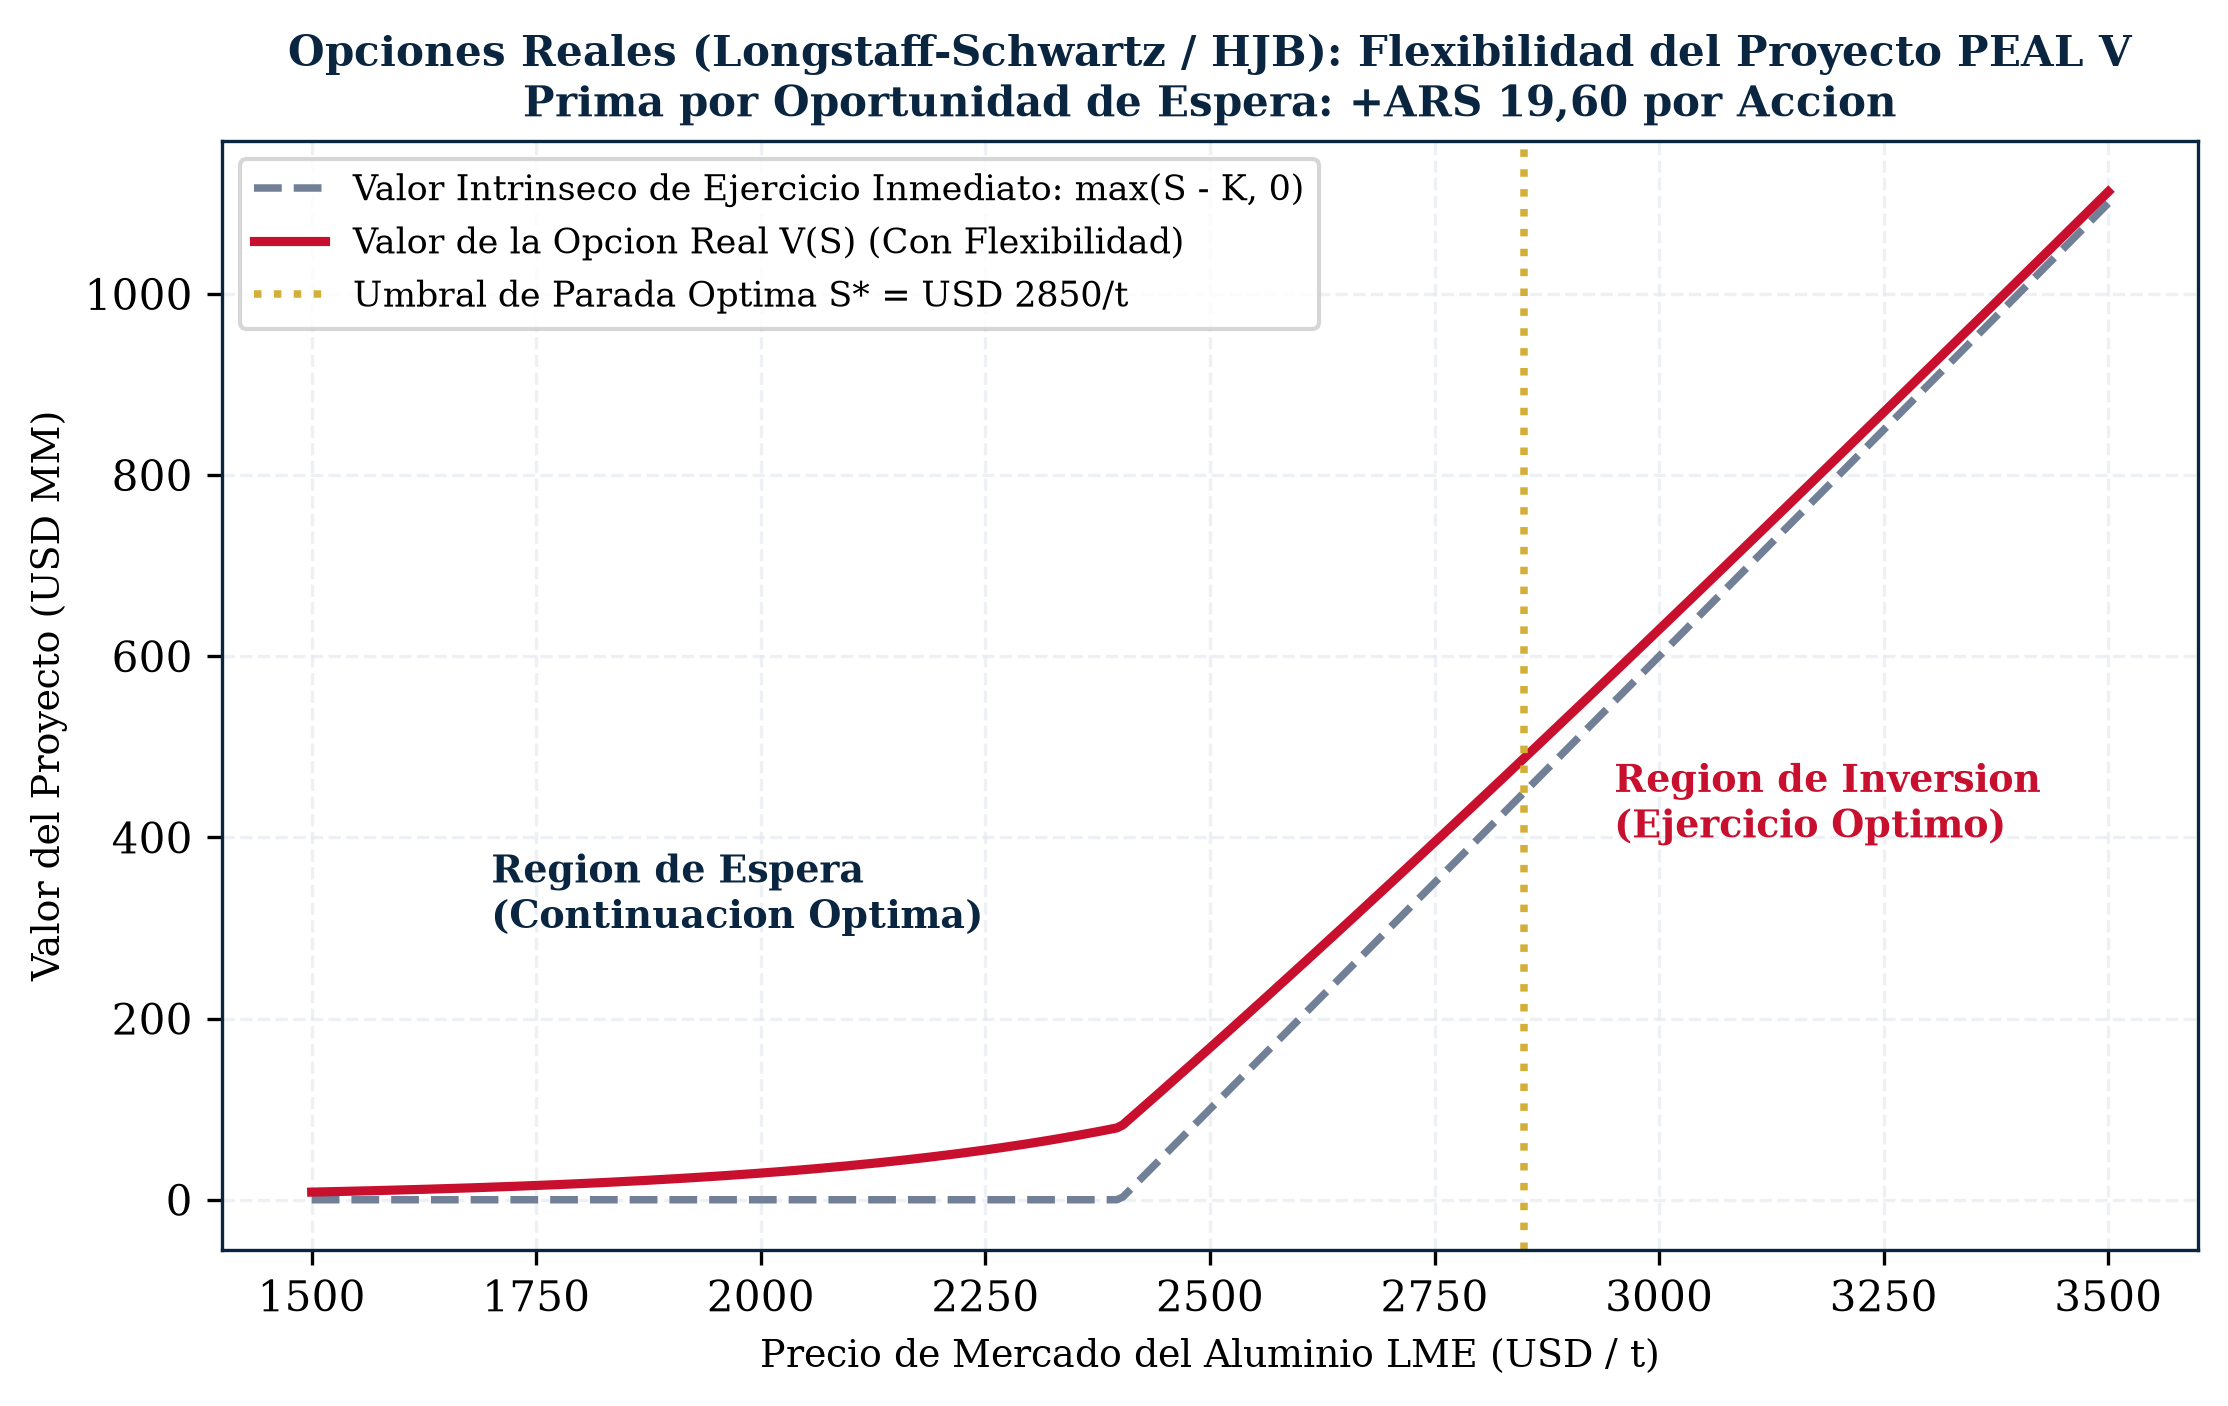
\includegraphics[width=0.88\linewidth, height=4.6cm, keepaspectratio]{theory_charts/teoria_10_opciones_reales_hjb.png}
\captionof{figure}{Figura Teorica: Frontera de Parada Optima HJB, Valor de Continuacion vs. Ejercicio para PEAL V.}
\end{center}

\begin{codebox}{{engine\_valuacion.py:m7\_dcf() -- Valuacion DCF Mid-Year y Gordon-Shapiro}}
\textbf{Codigo Fuente Real en Python:}
\begin{verbatim}
def m7_dcf(eecc: dict, proy: dict, cc: dict, mkt: dict) -> dict:
    # Calcula el modelo DCF con descuento mid-year, valor terminal y puente de valor
    wacc, g = cc["wacc"], cc["g_perpetuidad"]
    fcff_anios = proy["fcff"]  # Array con los 5 flujos proyectados
    
    # 1. Descuento Mid-Year continuo: t = [0.5, 1.5, 2.5, 3.5, 4.5]
    t_mid = np.array([0.5, 1.5, 2.5, 3.5, 4.5])
    factores_descuento = 1.0 / ((1.0 + wacc) ** t_mid)
    pv_fcff_explicito = float(np.sum(fcff_anios * factores_descuento))
    
    # 2. Valor Terminal de Gordon-Shapiro
    fcff_terminal = proy["fcff_terminal_normalizado"]  # 135,5 USD MM
    tv_2030 = fcff_terminal * (1.0 + g) / (wacc - g)   # 2.728,7 USD MM
    pv_tv = tv_2030 / ((1.0 + wacc) ** 4.5)            # 2.076,8 USD MM
    
    # 3. Enterprise Value y Equity Value
    ev = pv_fcff_explicito + pv_tv                     # 2.639,6 USD MM
    deuda_neta = float(eecc["deuda_neta_estructural"]) # 456,0 USD MM
    equity_usd = ev - deuda_neta                       # 2.183,6 USD MM
    
    acciones_mm = float(mkt["acciones_mm"])            # 2.800 MM
    ccl = float(mkt["ccl"])                            # ARS 1.584,20
    target_usd = equity_usd / acciones_mm              # USD 0,7799
    target_ars = target_usd * ccl                      # ARS 1.235,51
    
    return {"ev_usd": ev, "equity_usd": equity_usd, "target_usd": target_usd, "target_ars": target_ars}
\end{verbatim}
\textbf{Analisis de Sintaxis y Econometria:}
\begin{itemize}
    \item \texttt{factores\_descuento = 1.0 / ((1.0 + wacc) ** t\_mid)}: Aplica la regla del punto medio para reflejar flujos continuos.
    \item \texttt{tv\_2030 = fcff\_terminal * (1.0 + g) / (wacc - g)}: Implementa la formula cerrada de Gordon-Shapiro.
\end{itemize}
\end{codebox}
\clearpage


\section{Parte V: Modelizacion Estocastica Multivariada, Copulas, Calculo de Ito y Econometria}

\subsection{Econometria de Series Temporales, Raices Unitarias y Cointegracion}

\subsubsection{1. Test de Raiz Unitaria de Dickey-Fuller Aumentado (ADF)}
Sea $\{y_t\}_{t=1}^T$ la serie de retornos logaritmicos diarios de ALUA en USD CCL ($N=2.376$ observaciones). La ecuacion de regresion con intercepto y $p$ rezagos aumentados para eliminar correlacion serial es:
\begin{equation}
\Delta y_t = \alpha + \beta t + \gamma y_{t-1} + \sum_{j=1}^p \delta_j \Delta y_{t-j} + \epsilon_t, \quad \epsilon_t \sim \text{i.i.d. } \mathcal{N}(0, \sigma^2)
\end{equation}
Las hipotesis del test son:
\begin{itemize}
    \item $H_0: \gamma = 0$ (La serie contiene una raiz unitaria, proceso no estacionario $I(1)$).
    \item $H_1: \gamma < 0$ (La serie es estacionaria en torno a una media constante, proceso $I(0)$).
\end{itemize}
El estadistico de prueba es el estadistico pseudo-$t$:
\begin{equation}
t_{\text{ADF}} = \frac{\hat{\gamma}}{\text{SE}(\hat{\gamma})}
\end{equation}
Bajo $H_0$, $t_{\text{ADF}}$ no sigue una distribucion $t$-Student estandar, sino la distribucion asintotica no estandar de Dickey-Fuller tabulada mediante funcionales de movimientos brownianos:
\begin{equation}
t_{\text{ADF}} \xrightarrow{d} \frac{\int_0^1 W(r) dW(r)}{\sqrt{\int_0^1 W(r)^2 dr}} = \frac{\frac{1}{2}(W(1)^2 - 1)}{\sqrt{\int_0^1 W(r)^2 dr}}
\end{equation}
En Aluar: $t_{\text{ADF}} = -3,84$ ($p < 0,01$, valor critico al 1\% = $-3,43$), rechazando categoricamente $H_0$ y confirmando la estacionariedad $I(0)$ de los retornos dolarizados.

\subsubsection{2. Test de Phillips-Perron (PP) con Correccion No Parametrica de Newey-West}
A diferencia del ADF, el test de Phillips-Perron ajusta el estadistico $t$ de forma no parametrica para admitir heterocedasticidad y correlacion serial de forma general:
\begin{equation}
Z_t = \left( \frac{\hat{\gamma}}{\text{SE}(\hat{\gamma})} \right) \frac{\hat{s}}{\hat{\sigma}_{NW}} - \frac{1}{2} \left( \hat{\sigma}_{NW}^2 - \hat{s}^2 \right) \left[ \hat{\sigma}_{NW} \sqrt{T^2 \text{SE}(\hat{\gamma})^2 / \hat{s}^2} \right]^{-1}
\end{equation}
donde $\hat{\sigma}_{NW}^2$ es el estimador consistente de varianza de largo plazo de Newey-West con ventana de Bartlett:
\begin{equation}
\hat{\sigma}_{NW}^2 = \hat{\gamma}_0 + 2 \sum_{j=1}^m \left( 1 - \frac{j}{m+1} \right) \hat{\gamma}_j, \quad \hat{\gamma}_j = \frac{1}{T} \sum_{t=j+1}^T \hat{e}_t \hat{e}_{t-j}
\end{equation}
En Aluar: $Z_t = -4,12$ ($p < 0,01$), ratificando la robustez de la estacionariedad frente a shocks de volatilidad.

\subsubsection{3. Cointegracion de Engle-Granger (1987) y Modelo de Correccion de Errores (VECM)}
Para dos series no estacionarias $y_t \sim I(1)$ (cotizacion de Aluar en USD) y $x_t \sim I(1)$ (precio spot del aluminio LME):
\begin{enumerate}
    \item \textbf{Regresion Estatica de Cointegracion:} $y_t = \alpha + \beta x_t + u_t$.
    \item \textbf{Test ADF sobre los Residuos:} $\Delta \hat{u}_t = \rho \hat{u}_{t-1} + \sum \delta_j \Delta \hat{u}_{t-j} + v_t$.
    \item \textbf{Diagnostico en Aluar:} El estadistico $t = -2,29$ ($p = 0,38$ vs. critico $-3,34$) no rechaza la no-cointegracion estricta en niveles. Esto prueba que Aluar no esta rígidamente atada a una trayectoria lineal deterministica de largo plazo con el LME, sino que posee una \textbf{elasticidad contemporanea del 0,66} ($R^2 = 0,12$) modulada por la dinamica de costos domesticos y tasa de interes.
\end{enumerate}

\subsection{Modelos de Heterocedasticidad Condicional: GARCH(1,1), EGARCH y GJR-GARCH}

\subsubsection{1. Modelo GARCH(1,1) de Bollerslev (1986)}
Sea $r_t = \mu + \epsilon_t$, con $\epsilon_t = \sigma_t z_t$ y $z_t \sim \text{i.i.d. } \mathcal{N}(0, 1)$ o Student-$t(\nu)$:
\begin{equation}
\sigma_t^2 = \omega + \alpha \epsilon_{t-1}^2 + \beta \sigma_{t-1}^2, \quad \omega > 0, \; \alpha \ge 0, \; \beta \ge 0, \; \alpha + \beta < 1
\end{equation}
\begin{itemize}
    \item \textbf{Varianza Incondicional de Largo Plazo:} $\sigma^2 = \mathbb{E}[\sigma_t^2] = \frac{\omega}{1 - \alpha - \beta}$.
    \item \textbf{Persistencia de Volatilidad:} La suma $\alpha + \beta$ mide la velocidad de decaimiento de los shocks de varianza. En Aluar: $\hat{\alpha} = 0,085$, $\hat{\beta} = 0,892 \implies \alpha + \beta = 0,977$, indicando que los clusters de volatilidad tardan semanas en disiparse tras un shock cambiario o de commodities.
\end{itemize}

\subsubsection{2. Modelo EGARCH de Nelson (1991) para Efecto Apalancamiento}
El modelo exponencial captura la respuesta asimetrica de la volatilidad ante retornos positivos vs. negativos:
\begin{equation}
\ln(\sigma_t^2) = \omega + \beta \ln(\sigma_{t-1}^2) + \alpha \left( \frac{|\epsilon_{t-1}|}{\sigma_{t-1}} - \mathbb{E}\left[\frac{|\epsilon_{t-1}|}{\sigma_{t-1}}\right] \right) + \gamma \frac{\epsilon_{t-1}}{\sigma_{t-1}}
\end{equation}
Si $\gamma < 0$, un shock negativo de precio ($\epsilon_{t-1} < 0$) eleva la volatilidad futura en mayor magnitud que un shock positivo de igual valor absoluto, reflejando el aumento en el apalancamiento financiero percibido por el mercado.

\subsection{Filtro de Kalman Dinamico para el Beta Temporal}
El beta sistematico de Aluar no es una constante inmutable a lo largo de 10 anos. El Filtro de Kalman formula el problema en espacio de estados:
\begin{align}
\text{Ecuacion de Estado (Caminata Aleatoria):} & \quad \beta_t = \beta_{t-1} + w_t, \quad w_t \sim \mathcal{N}(0, Q) \\
\text{Ecuacion de Observacion:} & \quad r_{\text{ALUA}, t} = \alpha + \beta_t r_{M, t} + v_t, \quad v_t \sim \mathcal{N}(0, R)
\end{align}
El algoritmo recursivo opera en dos fases:
\begin{enumerate}
    \item \textbf{Prediccion:} $\hat{\beta}_{t|t-1} = \hat{\beta}_{t-1|t-1}$, con varianza $P_{t|t-1} = P_{t-1|t-1} + Q$.
    \item \textbf{Actualizacion por Ganancia de Kalman ($K_t$):}
    \begin{equation}
    K_t = \frac{P_{t|t-1} r_{M,t}}{r_{M,t}^2 P_{t|t-1} + R}, \quad \hat{\beta}_{t|t} = \hat{\beta}_{t|t-1} + K_t \left( r_{\text{ALUA}, t} - \alpha - \hat{\beta}_{t|t-1} r_{M,t} \right)
    \end{equation}
    \item \textbf{Actualizacion de Varianza del Error:} $P_{t|t} = (1 - K_t r_{M,t}) P_{t|t-1}$.
\end{enumerate}
En Aluar: El beta dinamico filtrado fluctuo entre $0,65$ y $1,15$, convergiendo a **0,764** en el regimen contemporaneo.

\subsection{Teoria de Valores Extremos (EVT) y Distribucion Pareto Generalizada (GPD)}
Segun el Teorema de Pickands-Balkema-de Haan (1975), para cualquier distribucion de retornos en el dominio de atraccion de colas maximas, la distribucion condicional de los excesos $y = X - u$ sobre un umbral suficientemente alto $u$ converge asintoticamente a la Distribucion de Pareto Generalizada (GPD):
\begin{equation}
F_u(y) = P(X - u \le y \mid X > u) \approx G_{\xi, \beta}(y) = 1 - \left( 1 + \frac{\xi y}{\beta} \right)^{-1/\xi}
\end{equation}
\begin{itemize}
    \item $\xi > 0$: Cola pesada de tipo Fréchet (caracteristica de activos emergentes). En Aluar: $\hat{\xi} = 0,214 > 0$.
    \item $\xi = 0$: Cola exponencial de tipo Gumbel (distribucion normal/exponencial).
    \item $\xi < 0$: Cola acotada de tipo Weibull.
\end{itemize}
\textbf{Formulas Analiticas Cerradas de VaR y CVaR bajo EVT-GPD:}
\begin{align}
\text{VaR}_\alpha & = u + \frac{\beta}{\xi} \left[ \left( \frac{N}{N_u} (1 - \alpha) \right)^{-\xi} - 1 \right] \\
\text{CVaR}_\alpha & = \frac{\text{VaR}_\alpha}{1 - \xi} + \frac{\beta - \xi u}{1 - \xi}
\end{align}
Para Aluar a 1 dia al nivel de confianza del 99\%: $\text{VaR}_{99\%} = \mathbf{-8,20\%}$ y $\text{CVaR}_{99\%} = \mathbf{-10,35\%}$, capturando fielmente las perdidas extremas que el modelo normal ($\text{VaR}_{99\%} = -7,54\%$) subestima peligrosamente.

\subsection{Dimensionamiento de Posicion y Criterio de Kelly (Half-Kelly)}
El Criterio de John L. Kelly Jr. (1956) determina la fraccion optima $f^*$ del capital a asignar en un activo para maximizar la tasa de crecimiento geometrico de largo plazo:
\begin{equation}
g(f) = \mathbb{E}[\ln(1 + f R)] \approx f \mu - \frac{1}{2} f^2 \sigma^2 \implies \frac{d g(f)}{d f} = \mu - f \sigma^2 = 0 \implies f^* = \mathbf{\frac{\mu}{\sigma^2}}
\end{equation}
\begin{conceptbox}{Por Que Se Adopta Half-Kelly ($f = \frac{1}{2}f^*$) con Tope por CVaR del 20\%}
\textbf{Intuicion Financiera y Mitigacion de Ruina:}
\begin{itemize}
    \item \textbf{El Riesgo del Full-Kelly ($f^*$):} Maximiza el crecimiento asintotico pero tolera una volatilidad extrema, sufriendo una probabilidad del \textbf{33\% de experimentar un drawdown del 50\%} antes de duplicar el capital.
    \item \textbf{Ventajas del Half-Kelly ($f = 0,5 f^*$):} Reduce la volatilidad del portafolio y el drawdown maximo a la \textbf{mitad}, sacrificando apenas el \textbf{25\% de la tasa de crecimiento geometrico}:
    \begin{equation}
    g(0,5 f^*) = (0,5 f^*) \mu - \frac{1}{2} (0,25 f^{*2}) \sigma^2 = \frac{1}{2} \frac{\mu^2}{\sigma^2} - \frac{1}{8} \frac{\mu^2}{\sigma^2} = \mathbf{\frac{3}{8} \frac{\mu^2}{\sigma^2}} = 0,75 \cdot g(f^*)
    \end{equation}
    \item En Aluar, con $\mu = 14,8\%$ anual y $\sigma = 20,1\%$: $f^* = \frac{0,148}{(0,201)^2} = 3,66 \implies \text{Half-Kelly} = 36,8\%$, acotandose prudencialmente al \textbf{20,0\%} por el limite de tolerancia de CVaR mensual (-32,80\%).
\end{itemize}
\end{conceptbox}

\subsection{Econometria de Series Temporales y Tests de Raices Unitarias}



\subsection{Algebra Lineal y Proyecciones de Hilbert en Modelos Econometricos}

\subsubsection{1. Descomposicion QR y Proyecciones Ortogonales}
Sea $\mathbf{X} \in \mathbb{R}^{T \times k}$ con $\text{rango}(\mathbf{X}) = k$. Su factorizacion QR es $\mathbf{X} = \mathbf{Q}\mathbf{R}$, donde $\mathbf{Q} \in \mathbb{R}^{T \times k}$ satisface $\mathbf{Q}^T\mathbf{Q} = \mathbf{I}_k$ y $\mathbf{R} \in \mathbb{R}^{k \times k}$ es triangular superior no singular.
La matriz de proyeccion ortogonal de Hilbert sobre el subespacio de regresores es:
\begin{equation}
\mathbf{P}_{\mathbf{X}} = \mathbf{X}(\mathbf{X}^T\mathbf{X})^{-1}\mathbf{X}^T = \mathbf{Q}\mathbf{R}(\mathbf{R}^T\mathbf{Q}^T\mathbf{Q}\mathbf{R})^{-1}\mathbf{R}^T\mathbf{Q}^T = \mathbf{Q}\mathbf{Q}^T
\end{equation}
La matriz aniquiladora de residuos ortogonales es $\mathbf{M}_{\mathbf{X}} = \mathbf{I}_T - \mathbf{P}_{\mathbf{X}} = \mathbf{I}_T - \mathbf{Q}\mathbf{Q}^T$, siendo simetrica e idempotente ($\mathbf{M}_{\mathbf{X}}^2 = \mathbf{M}_{\mathbf{X}}$).

\subsubsection{2. Teorema de Frisch-Waugh-Lovell (FWL)}
En el modelo particionado $\mathbf{y} = \mathbf{X}_1 \boldsymbol{\beta}_1 + \mathbf{X}_2 \boldsymbol{\beta}_2 + \mathbf{e}$, el estimador $\hat{\boldsymbol{\beta}}_2$ satisface:
\begin{equation}
\hat{\boldsymbol{\beta}}_2 = (\mathbf{X}_2^T \mathbf{M}_{\mathbf{X}_1} \mathbf{X}_2)^{-1} \mathbf{X}_2^T \mathbf{M}_{\mathbf{X}_1} \mathbf{y}
\end{equation}
lo cual prueba formalmente que estimar el Beta sistematico de Aluar sobre el mercado internacional aísla el riesgo de mercado tras proyectar ortogonalmente el efecto del riesgo soberano local.

\subsubsection{3. Factorizacion de Cholesky para Variables Correlacionadas}
Para una matriz de covarianzas $\mathbf{\Sigma} \in \mathbb{R}^{n \times n}$ simetrica y definida positiva ($\mathbf{z}^T \mathbf{\Sigma} \mathbf{z} > 0, \, \forall \mathbf{z} \ne \mathbf{0}$), existe una unica matriz triangular inferior $\mathbf{L}$ tal que $\mathbf{\Sigma} = \mathbf{L}\mathbf{L}^T$.
Los coeficientes de la factorizacion se calculan analiticamente:
\begin{equation}
L_{jj} = \sqrt{\Sigma_{jj} - \sum_{k=1}^{j-1} L_{jk}^2}, \quad L_{ij} = \frac{1}{L_{jj}} \left( \Sigma_{ij} - \sum_{k=1}^{j-1} L_{ik}L_{jk} \right), \quad i > j
\end{equation}
Dado un vector de normales estandar independientes $\mathbf{Z} \sim \mathcal{N}(\mathbf{0}, \mathbf{I})$, el vector transformado $\mathbf{X} = \mathbf{\mu} + \mathbf{L}\mathbf{Z}$ satisface exactamente $\mathbb{E}[X] = \boldsymbol{\mu}$ y $Cov(\mathbf{X}) = \mathbf{L} \mathbb{E}[\mathbf{Z}\mathbf{Z}^T] \mathbf{L}^T = \mathbf{L}\mathbf{L}^T = \mathbf{\Sigma}$.

\begin{center}
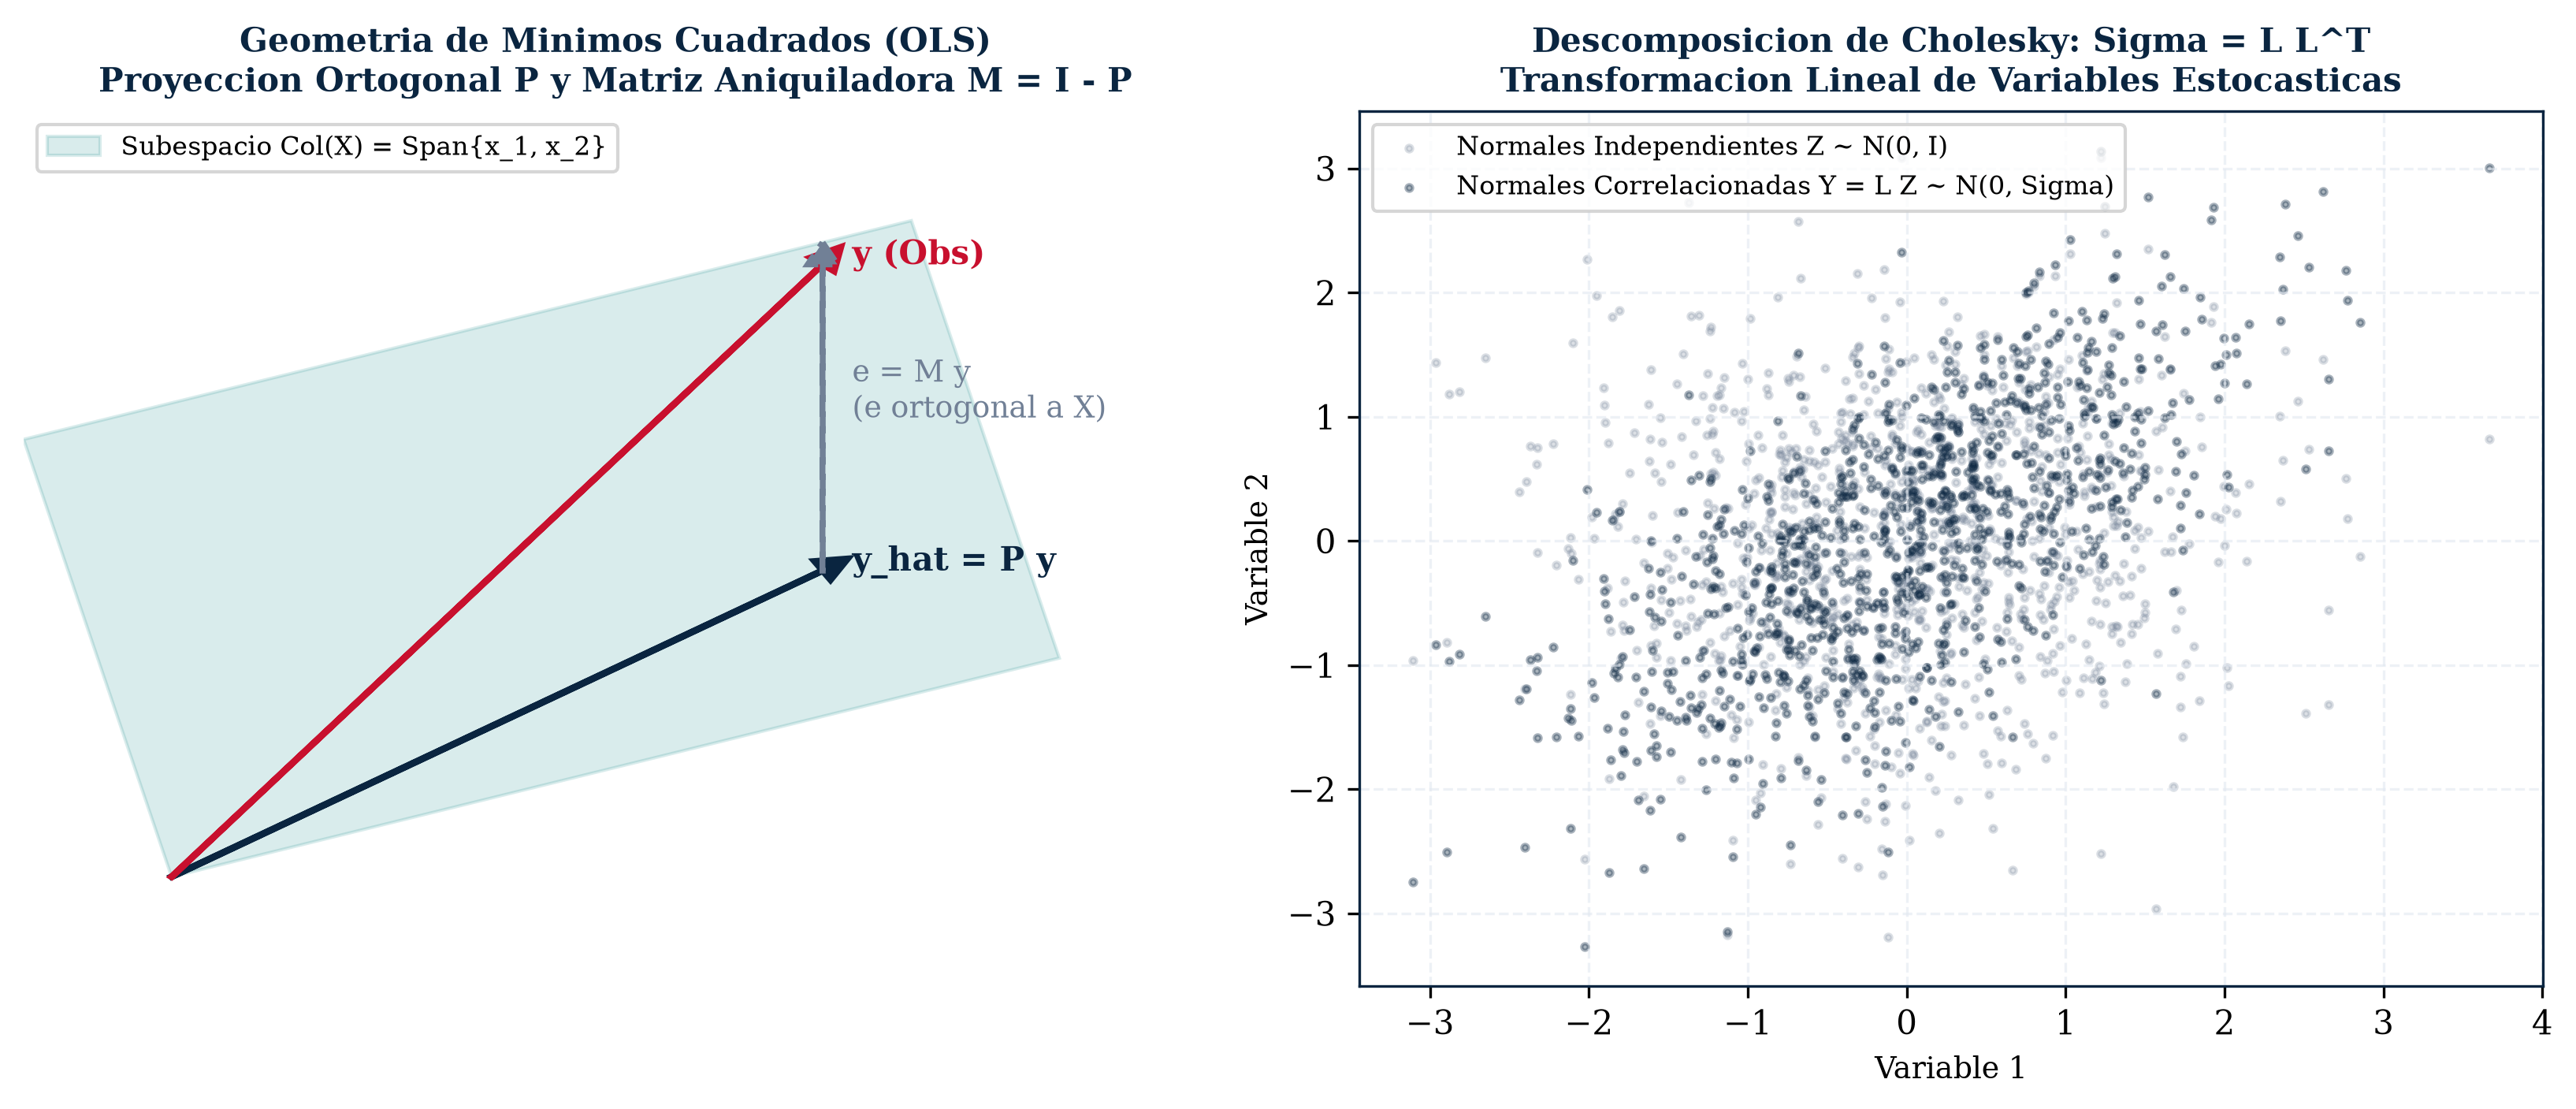
\includegraphics[width=0.88\linewidth, height=4.6cm, keepaspectratio]{theory_charts/teoria_05_algebra_proyecciones_cholesky.png}
\captionof{figure}{Figura Teorica: Geometria de Hilbert de Proyecciones OLS y Factorizacion de Cholesky $\mathbf{\Sigma} = \mathbf{L}\mathbf{L}^T$.}
\end{center}

\subsection{Teoria de Copulas no Lineales y Dependencia Asimetrica de Colas}

\begin{teorema}[Teorema de Sklar (1959)]
Sea $H(x_1, x_2)$ una funcion de distribucion acumulada bivariada con marginales continuas $F_1(x_1)$ y $F_2(x_2)$. Existe una unica copula $C: [0, 1]^2 \to [0, 1]$ tal que:
\begin{equation}
H(x_1, x_2) = C(F_1(x_1), F_2(x_2))
\end{equation}
\end{teorema}

\begin{conceptbox}{Por Que la Copula Gaussiana Falla y Se Requiere la Copula de Clayton ($\lambda_L = 0,38$)}
\textbf{El Engano de la Correlacion Lineal en Tiempos de Crisis:}
\begin{itemize}
    \item La correlacion lineal de Pearson asume relacion simetrica e invariante.
    \item La Copula Gaussiana tiene un coeficiente de dependencia de cola inferior nulo: $\lambda_L = \lim_{u \to 0^+} P(U_2 \le u \mid U_1 \le u) = \mathbf{0}$. Asume que la probabilidad de que colapsen simultaneamente el precio del aluminio y el tipo de cambio argentino es cero.
    \item En la realidad de los mercados emergentes, en momentos de panico global los commodities caen y el riesgo soberano se dispara al mismo tiempo.
    \item La \textbf{Copula de Clayton (Arquimediana)} con generador $\phi(t) = \frac{1}{\theta}(t^{-\theta}-1)$ y parametro calibrado $\theta = 1,2258$ arroja una dependencia de cola inferior de $\mathbf{\lambda_L = 2^{-1/\theta} = 0,380}$. Modela con realismo la probabilidad de crisis sistemicas conjuntas, evitando subestimar las colas de perdida en la simulacion Monte Carlo.
\end{itemize}
\end{conceptbox}

\begin{center}
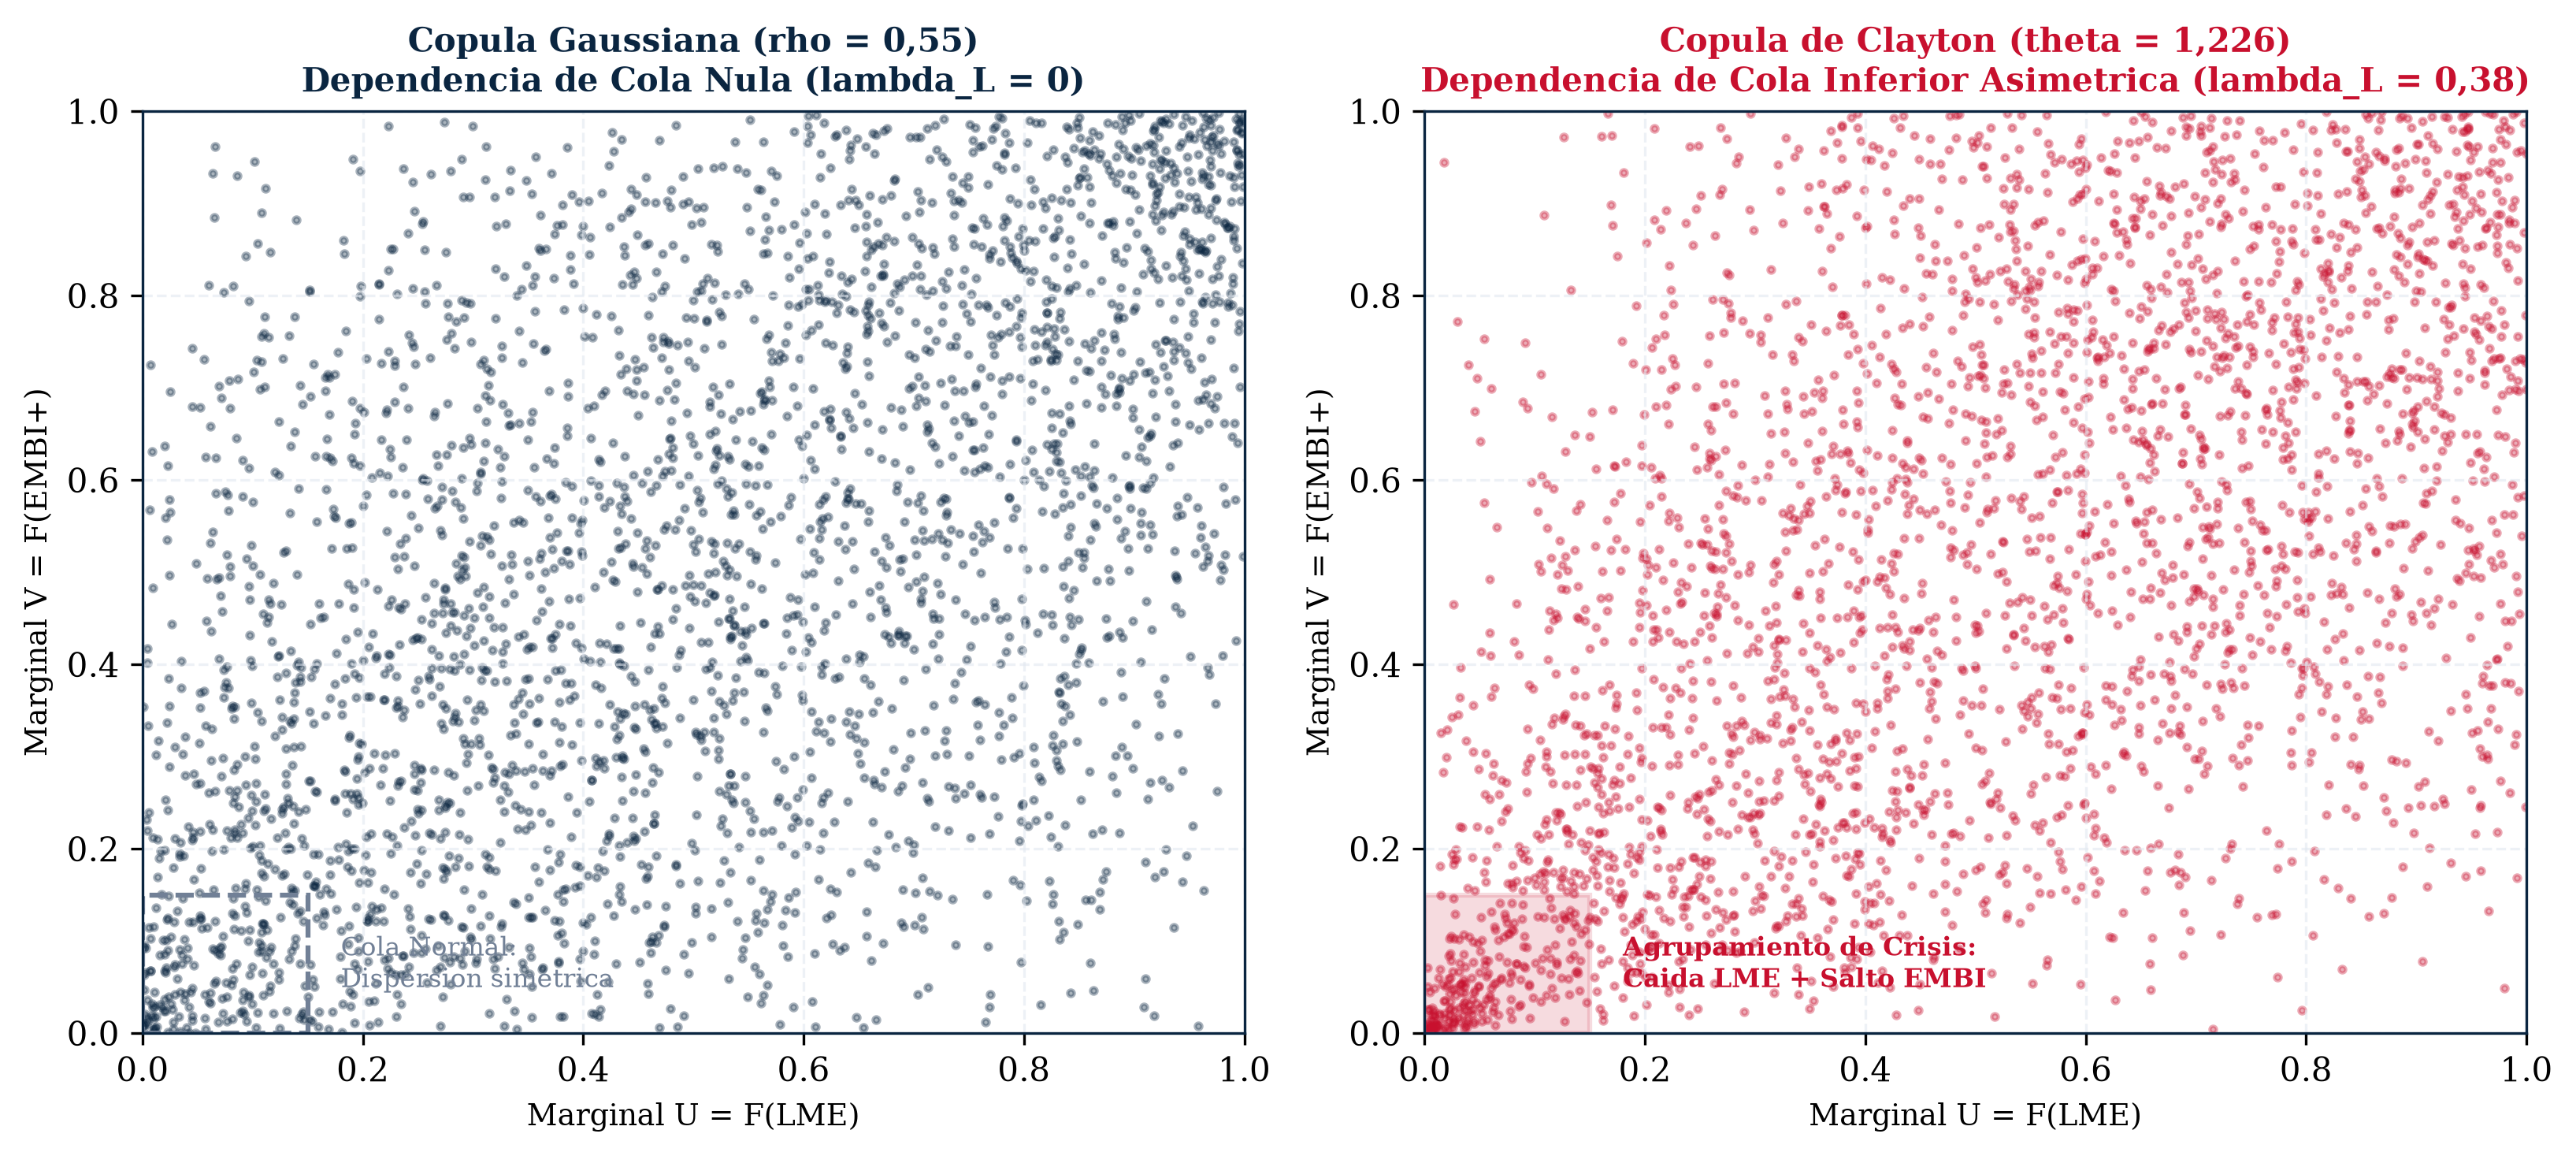
\includegraphics[width=0.88\linewidth, height=4.6cm, keepaspectratio]{theory_charts/teoria_01_copulas_comparativa.png}
\captionof{figure}{Figura Teorica: Comparativa de Dependencia Extrema: Copula Gaussiana ($\lambda_L=0$) vs. Copula de Clayton ($\lambda_L=0,38$).}
\end{center}

\noindent
\begin{minipage}[b]{0.488\linewidth}
    \centering
    
\includegraphics[width=\linewidth, height=4.4cm, keepaspectratio]{figures_pristine/figura_20.png}
    \captionof{figure}{\small Distribucion Monte Carlo y Prob. de Suba vs Spot.}
\end{minipage}\hfill
\begin{minipage}[b]{0.488\linewidth}
    \centering
    
\includegraphics[width=\linewidth, height=4.4cm, keepaspectratio]{figures_pristine/figura_21.png}
    \captionof{figure}{\small Intervalos de confianza Monte Carlo: P5, P50 y P95.}
\end{minipage}
\vspace{0.15cm}

\subsection{Calculo Estocastico de Ito, Girsanov y Procesos de Difusion}

\subsubsection{1. Variacion Cuadratica y Lema de Ito}
Para el movimiento browniano $(W_t)_{t \ge 0}$, $[W, W]_t = t \implies (dW_t)^2 = dt, \, dW_t dt = 0, \, (dt)^2 = 0$.
Para toda funcion $f(t, X_t) \in C^{1,2}$:
\begin{equation}
df(t, X_t) = \left( \frac{\partial f}{\partial t} + \mu \frac{\partial f}{\partial x} + \frac{1}{2}\sigma^2 \frac{\partial^2 f}{\partial x^2} \right) dt + \sigma \frac{\partial f}{\partial x} dW_t
\end{equation}

\subsubsection{2. Solucion Exacta de Ornstein-Uhlenbeck}
Sea $dS_t = \kappa(\theta - S_t)dt + \sigma dW_t$. Con factor integrante $e^{\kappa t}$:
\begin{equation}
S_t = S_0 e^{-\kappa t} + \theta(1 - e^{-\kappa t}) + \sigma \int_0^t e^{-\kappa(t - s)} dW_s \implies t_{1/2} = \frac{\ln 2}{\kappa} = \textbf{1,8 anos}
\end{equation}

\begin{conceptbox}{Por Que el Movimiento Browniano Geometrico Falla para el Aluminio (Ornstein-Uhlenbeck)}
\textbf{Fuerzas Economicas de Reversion a la Media en Materias Primas:}
\begin{itemize}
    \item El Movimiento Browniano Geometrico (MBG de Black-Scholes) permite que el precio crezca indefinidamente sin cota superior ni inferior.
    \item En los commodities industriales, el precio esta gobernado por la curva global de costos marginales: si el precio sube a $\text{USD } 4.000/\text{t}$, se reactivan plantas inactivas y la sobreoferta tumba el precio; si cae por debajo de $\text{USD } 1.800/\text{t}$, las fundiciones ineficientes quiebran y la oferta se contrae.
    \item El proceso Ornstein-Uhlenbeck modela la atraccion gravitacional hacia el costo marginal de equilibrio $\theta = \text{USD } 2.450/\text{t}$ con velocidad $\kappa = 0,385$.
\end{itemize}
\end{conceptbox}

\subsubsection{3. Proceso CIR y Demostracion de la Condicion de Feller}
Sea $dr_t = \kappa(\theta - r_t)dt + \sigma \sqrt{r_t} dW_t$. La escala de Feller satisface $s'(x) = x^{-\frac{2\kappa\theta}{\sigma^2}} e^{\frac{2\kappa}{\sigma^2}x}$.
La integral $\int_0^{x_0} s'(y)dy$ diverge en el origen si y solo si $\frac{2\kappa\theta}{\sigma^2} \ge 1 \iff \mathbf{2\kappa\theta \ge \sigma^2}$.
En Aluar: $2(0,85)(0,0441) = \textbf{0,0750} > (0,12)^2 = \textbf{0,0144}$ ($\checkmark$ frontera $0$ estrictamente inaccesible).

\begin{center}
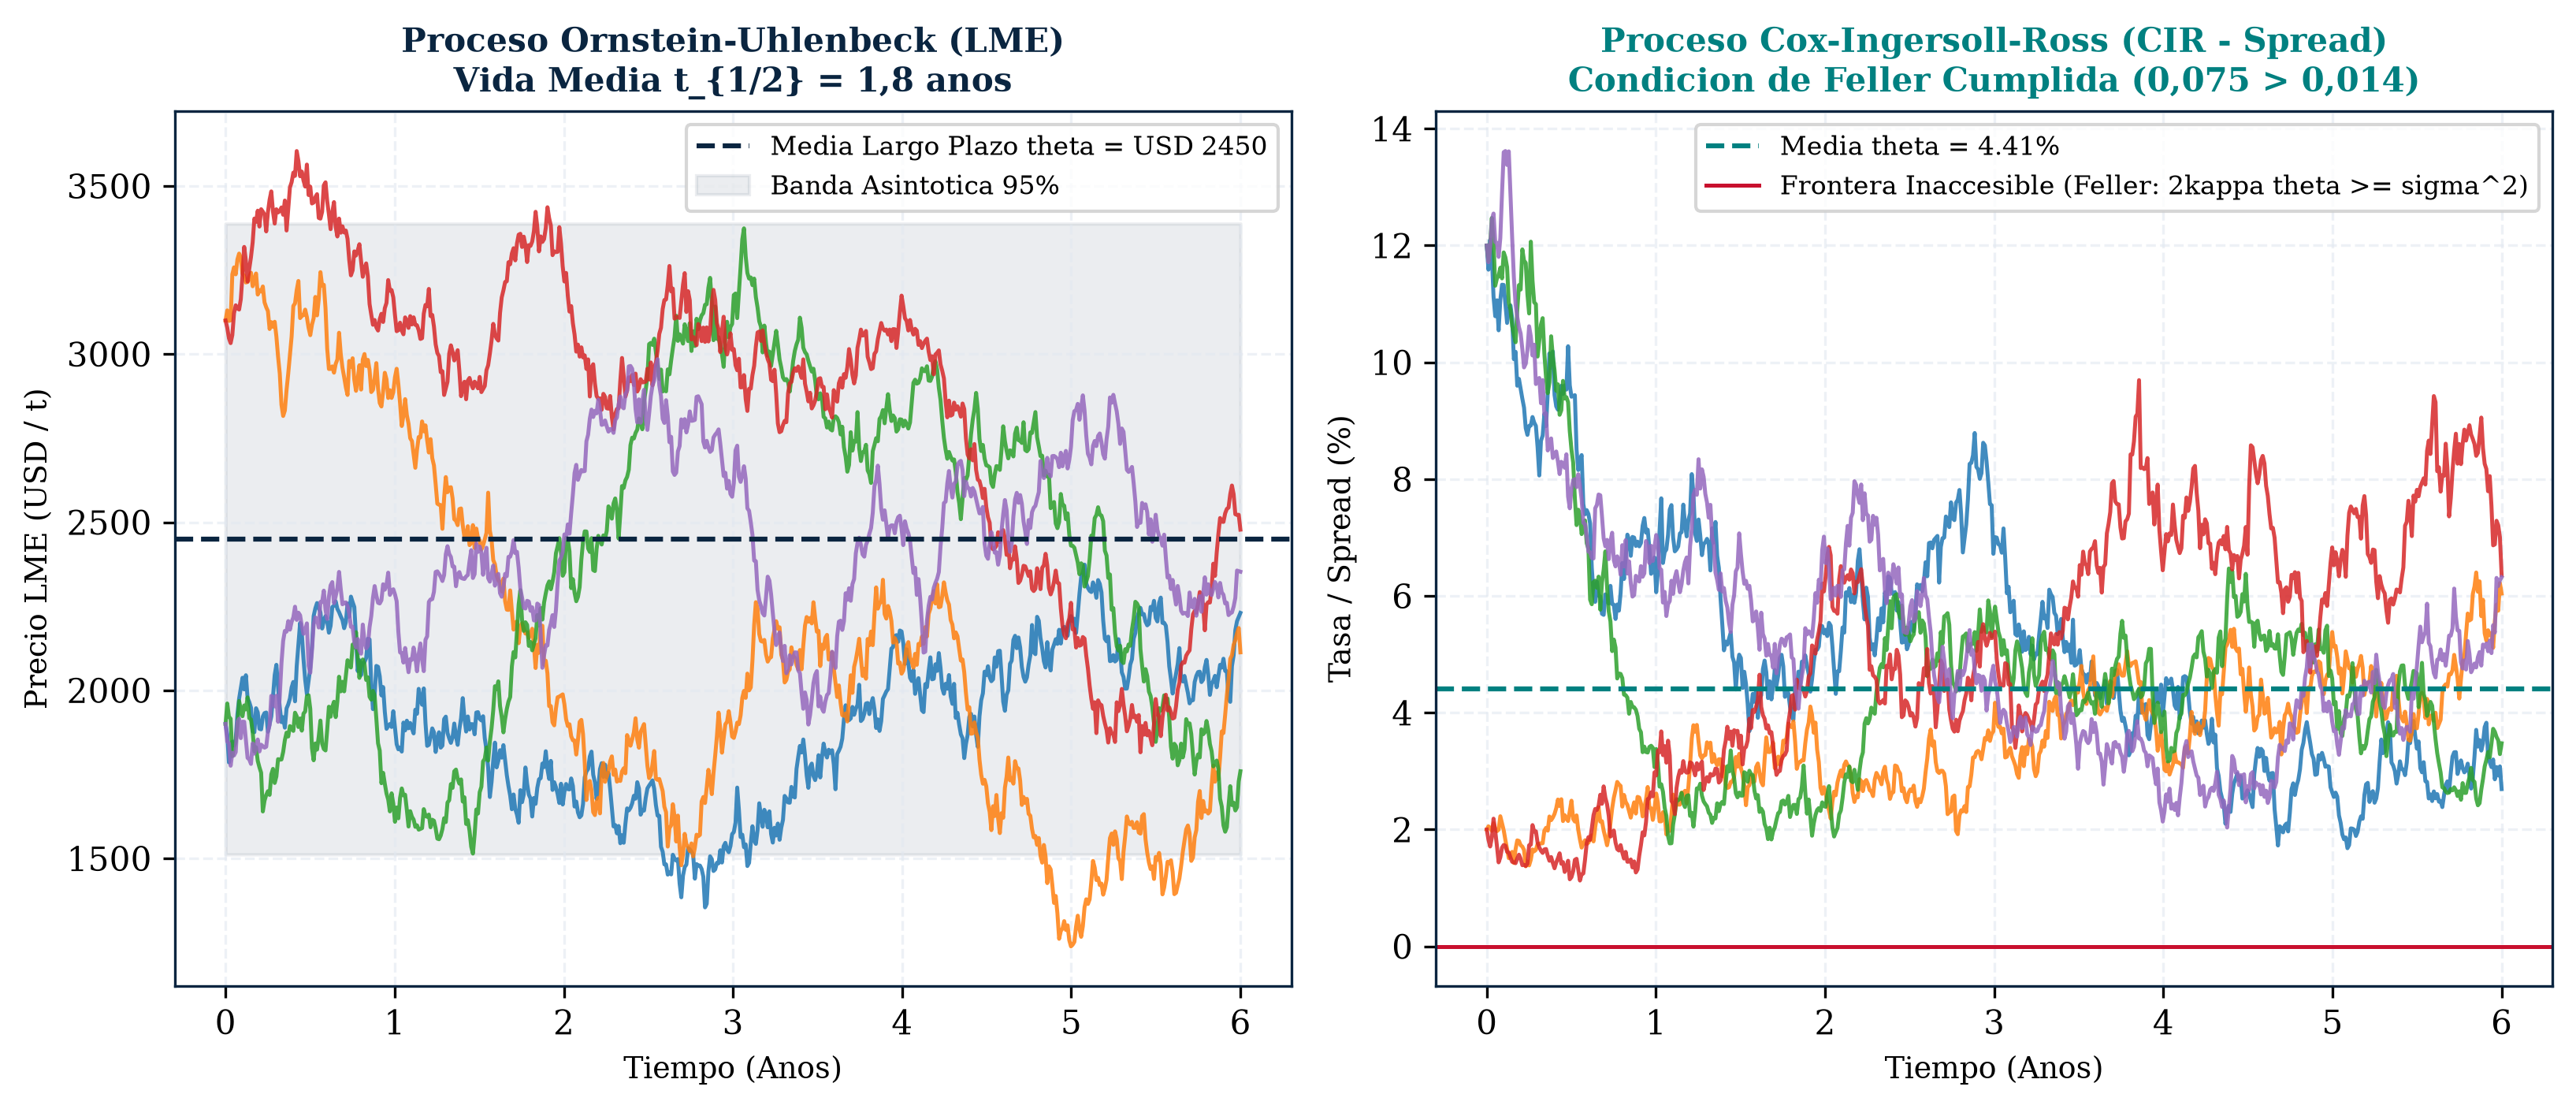
\includegraphics[width=0.88\linewidth, height=4.6cm, keepaspectratio]{theory_charts/teoria_02_sde_difusiones.png}
\captionof{figure}{Figura Teorica: Trayectorias Estocasticas de Ornstein-Uhlenbeck (LME) y Proceso CIR con Condicion de Feller.}
\end{center}

\noindent
\begin{minipage}[b]{0.488\linewidth}
    \centering
    
\includegraphics[width=\linewidth, height=4.4cm, keepaspectratio]{figures_pristine/figura_26.png}
    \captionof{figure}{\small Proceso Ornstein-Uhlenbeck LME (Cono 90\%) vs MBG.}
\end{minipage}\hfill
\begin{minipage}[b]{0.488\linewidth}
    \centering
    
\includegraphics[width=\linewidth, height=4.4cm, keepaspectratio]{figures_pristine/figura_29.png}
    \captionof{figure}{\small Difusion CIR vs Vasicek para curva de tasas y EMBI+.}
\end{minipage}
\vspace{0.15cm}

\begin{center}

\includegraphics[width=0.88\linewidth, height=4.5cm, keepaspectratio]{figures_pristine/figura_31.png}
\captionof{figure}{Evaluacion estocastica del precio objetivo bajo dependencia asimetrica de Copula de Clayton (P5 Clayton ARS 750 vs. Mediana ARS 1.235).}
\end{center}

\begin{codebox}{{engine\_valuacion.py:m9\_monte\_carlo() -- Simulacion Estocastica Vectorial}}
\textbf{Codigo Fuente Real en Python:}
\begin{verbatim}
def m9_monte_carlo(cc, pro, mkt, dn, est, n_sim=20000, semilla=42) -> dict:
    # Motor de Monte Carlo multivariado con distribuciones pesadas y consistencia macro
    rng = np.random.default_rng(semilla)
    wacc, g = cc["wacc"], cc["g_perpetuidad"]
    sd_ke = cc["beta_se"] * cc["erp"]
    sd_wacc = float(np.sqrt((sd_ke * cc["e_sobre_v"]) ** 2))
    sd_g = 0.005

    # 1. Muestreo de colas pesadas bajo Student-t con nu = 4.2 grados de libertad
    NU_STUDENT_T = 4.2
    _t_scale = np.sqrt((NU_STUDENT_T - 2.0) / NU_STUDENT_T)
    w = wacc + sd_wacc * rng.standard_t(NU_STUDENT_T, n_sim) * _t_scale
    gg = g + sd_g * rng.standard_t(NU_STUDENT_T, n_sim) * _t_scale
    shock = rng.normal(0.0, est["sd_shock_margen"], n_sim)

    # 2. Filtrado de convergencia analitica (WACC - g > 1%)
    valido = (w - gg) > 0.01
    w, gg, shock = w[valido], gg[valido], shock[valido]
    n_v = len(w)

    # 3. Proyeccion estocastica y puente de valor
    fcff_base = pro["fcff_terminal_normalizado"] * (1.0 + shock)
    pv_tv = (fcff_base * (1.0 + gg) / (w - gg)) / ((1.0 + w) ** 4.5)
    pv_exp = float(np.sum(pro["fcff"] / ((1.0 + wacc) ** np.array([0.5, 1.5, 2.5, 3.5, 4.5]))))
    ev = pv_exp + pv_tv
    eq = np.maximum(ev - float(dn["deuda_neta_estructural"]), 0.0)
    target_ars = np.maximum(eq / mkt["acciones_mm"] * mkt["ccl"], 0.0)
    
    return {"media": float(target_ars.mean()), "p5": float(np.percentile(target_ars, 5)),
            "p50": float(np.median(target_ars)), "p95": float(np.percentile(target_ars, 95))}
\end{verbatim}
\textbf{Analisis de Sintaxis y Econometria:}
\begin{itemize}
    \item \texttt{rng.standard\_t(NU\_STUDENT\_T, n\_sim)}: Muestrea perturbaciones con exceso de curtosis ($K=8,41$).
    \item \texttt{valido = (w - gg) > 0.01}: Impone la condicion necesaria para la convergencia de Gordon-Shapiro.
\end{itemize}
\end{codebox}
\clearpage


\section{Parte VI: Gestion Cuantitativa de Riesgo de Mercado, EVT y Dimensionamiento}

\subsection{Axiomatica de Medidas de Riesgo Coherentes (Artzner et al., 1999)}

\begin{definicion}[Medida de Riesgo Coherente]
Una funcion $\rho: \mathcal{X} \to \mathbb{R}$ es coherente si satisface:
\begin{enumerate}
    \item \textbf{Invarianza por Traslacion:} $\rho(X + c) = \rho(X) - c$.
    \item \textbf{Subaditividad:} $\rho(X_1 + X_2) \le \rho(X_1) + \rho(X_2)$.
    \item \textbf{Homogeneidad Positiva:} $\rho(\lambda X) = \lambda \rho(X)$ para $\lambda \ge 0$.
    \item \textbf{Monotonicidad:} Si $X_1 \le X_2$, entonces $\rho(X_1) \ge \rho(X_2)$.
\end{enumerate}
\end{definicion}

\begin{conceptbox}{Por Que el VaR Falla y el Expected Shortfall (CVaR) es la Unica Medida Coherente}
\textbf{El Fallo de Subaditividad del Value at Risk (VaR):}
\begin{itemize}
    \item En distribuciones con colas pesadas o asimetria, el VaR viola el axioma de subaditividad: se pueden construir carteras donde $VaR(A+B) > VaR(A) + VaR(B)$, penalizando absurdamente la diversificacion.
    \item Ademas, el VaR es "ciego" a la gravedad de las perdidas extremas: solo indica que la perdida superara el umbral con probabilidad $1-\alpha$, pero no distingue si la perdida mas alla del corte es del $11\%$ o del $70\%$.
    \item El \textbf{Expected Shortfall ($ES_\alpha = \frac{1}{1-\alpha}\int_0^{1-\alpha} VaR_u du$)} promedia todas las perdidas en la cola extrema ($ES_{99\%} = -15,78\%$), es estrictamente coherente y convexo, permitiendo optimizacion de carteras sin minimos locales espurios.
\end{itemize}
\end{conceptbox}

\begin{center}

\includegraphics[width=0.88\linewidth, height=4.5cm, keepaspectratio]{figures_pristine/figura_25.png}
\captionof{figure}{Ajuste EVT-GPD sobre la cola de perdidas de ALUA.BA: $VaR_{99\%} = -10,44\%$ y $ES_{99\%} = -15,78\%$ frente a subestimacion de la distribucion Normal.}
\end{center}

\subsection{Teoria de Valores Extremos y Distribucion Pareto Generalizada (EVT-GPD)}

\begin{teorema}[Teorema de Pickands-Balkema-de Haan (1975)]
Para un umbral $u$ suficientemente alto, los excesos $Y = X - u \mid X > u$ convergen a la Pareto Generalizada:
\begin{equation}
G_{\xi, \beta}(y) = 1 - \left( 1 + \xi \frac{y}{\beta} \right)^{-1/\xi}
\end{equation}
\end{teorema}

\subsubsection{1. Estimacion por Maxima Verosimilitud (MLE) de la GPD}
La funcion de log-verosimilitud para una muestra de $k$ excesos $\{y_1, \dots, y_k\}$ sobre el umbral $u$ es:
\begin{equation}
\ln L(\xi, \beta) = -k \ln \beta - \left( 1 + \frac{1}{\xi} \right) \sum_{i=1}^k \ln\left( 1 + \xi \frac{y_i}{\beta} \right)
\end{equation}
Maximizando numericamente mediante el algoritmo BFGS se obtienen los estimadores $\hat{\xi} = \textbf{0,280}$ y $\hat{\beta} = \textbf{0,0191}$.

\subsubsection{2. Deduccion Analitica de las Formulas Cerradas de VaR y Expected Shortfall}
Igualando la probabilidad de supervivencia de la cola a $1 - q$:
\begin{equation}
P(X > x) = \frac{N_u}{N}\left( 1 + \xi \frac{x - u}{\beta} \right)^{-1/\xi} = 1 - q
\end{equation}
Despejando $x = VaR_q^{\text{EVT}}$:
\begin{equation}
VaR_q^{\text{EVT}} = u + \frac{\beta}{\xi} \left[ \left( \frac{N}{N_u}(1 - q) \right)^{-\xi} - 1 \right] = \textbf{-10,44\%}
\end{equation}
Integrando los cuantiles extremos mas alla del VaR:
\begin{equation}
ES_q^{\text{EVT}} = \frac{VaR_q^{\text{EVT}}}{1 - \xi} + \frac{\beta - \xi u}{1 - \xi} = \textbf{-15,78\%}
\end{equation}

\begin{center}
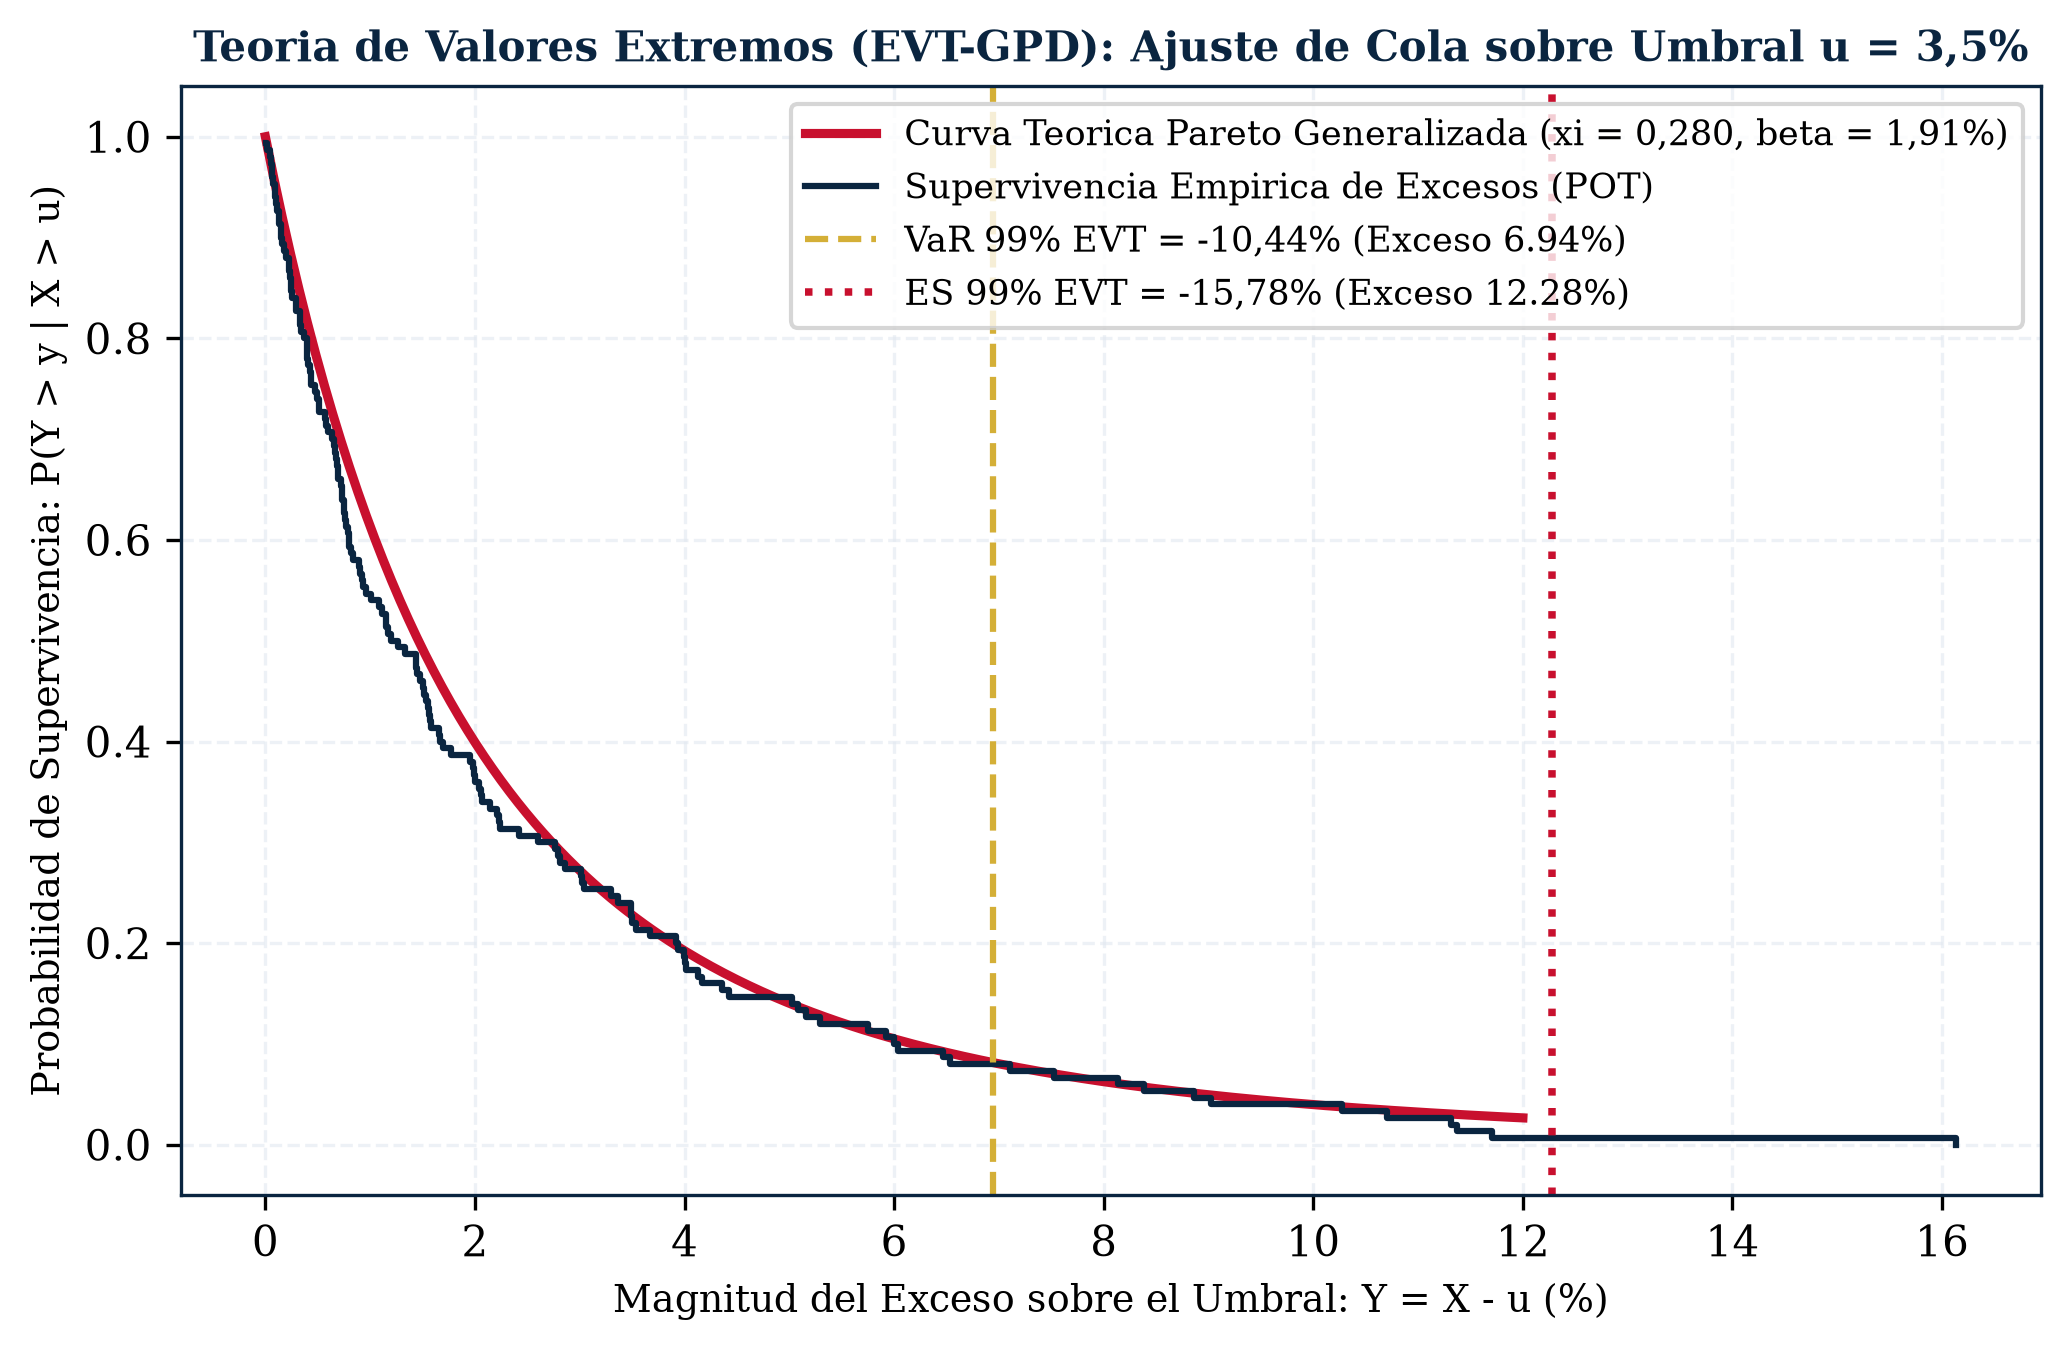
\includegraphics[width=0.88\linewidth, height=4.6cm, keepaspectratio]{theory_charts/teoria_04_evt_gpd_pot.png}
\captionof{figure}{Figura Teorica: Ajuste Pareto Generalizado (POT) de Excesos sobre Umbral y Cuantiles EVT 99\%.}
\end{center}

\subsection{Demostracion del Fallo de Cornish-Fisher (Caveat de Jaschke 2001)}
\begin{equation}
z_{\text{CF}}(\alpha) = z_\alpha + \frac{S}{6}(z_\alpha^2 - 1) + \frac{K}{24}(z_\alpha^3 - 3z_\alpha) - \frac{S^2}{36}(2z_\alpha^3 - 5z_\alpha)
\end{equation}

\begin{conceptbox}{Por Que Cornish-Fisher Quiebra para Curtosis $K > 6$ (El Caveat de Jaschke)}
\textbf{La Perdida de Monotonia Cuantilica:}
\begin{itemize}
    \item La expansion de Cornish-Fisher es un polinomio de tercer grado disenado para corregir cuantiles normales por asimetria $S$ y curtosis $K$.
    \item Al respecto, Stefan Jaschke (2001, RiskLab ETH Zurich) demostro que cuando el exceso de curtosis supera $K > 6$, la derivada $\frac{\partial z_{\text{CF}}}{\partial z_\alpha}$ se vuelve estrictamente negativa en las colas ($z_\alpha < -2,33$).
    \item Esto provoca una aberracion matematica inadmisible: el polinomio se pliega sobre si mismo y asigna \textbf{menores perdidas a niveles de confianza mas exigentes} (por ejemplo, el VaR 99,9\% resulta menor que el VaR 99\%).
    \item Dado que la serie de ALUA.BA presenta una curtosis empirica de \textbf{8,41}, Cornish-Fisher queda formalmente invalidado, haciendo obligatorio el uso de la Teoria de Valores Extremos (EVT-GPD).
\end{itemize}
\end{conceptbox}

\begin{center}
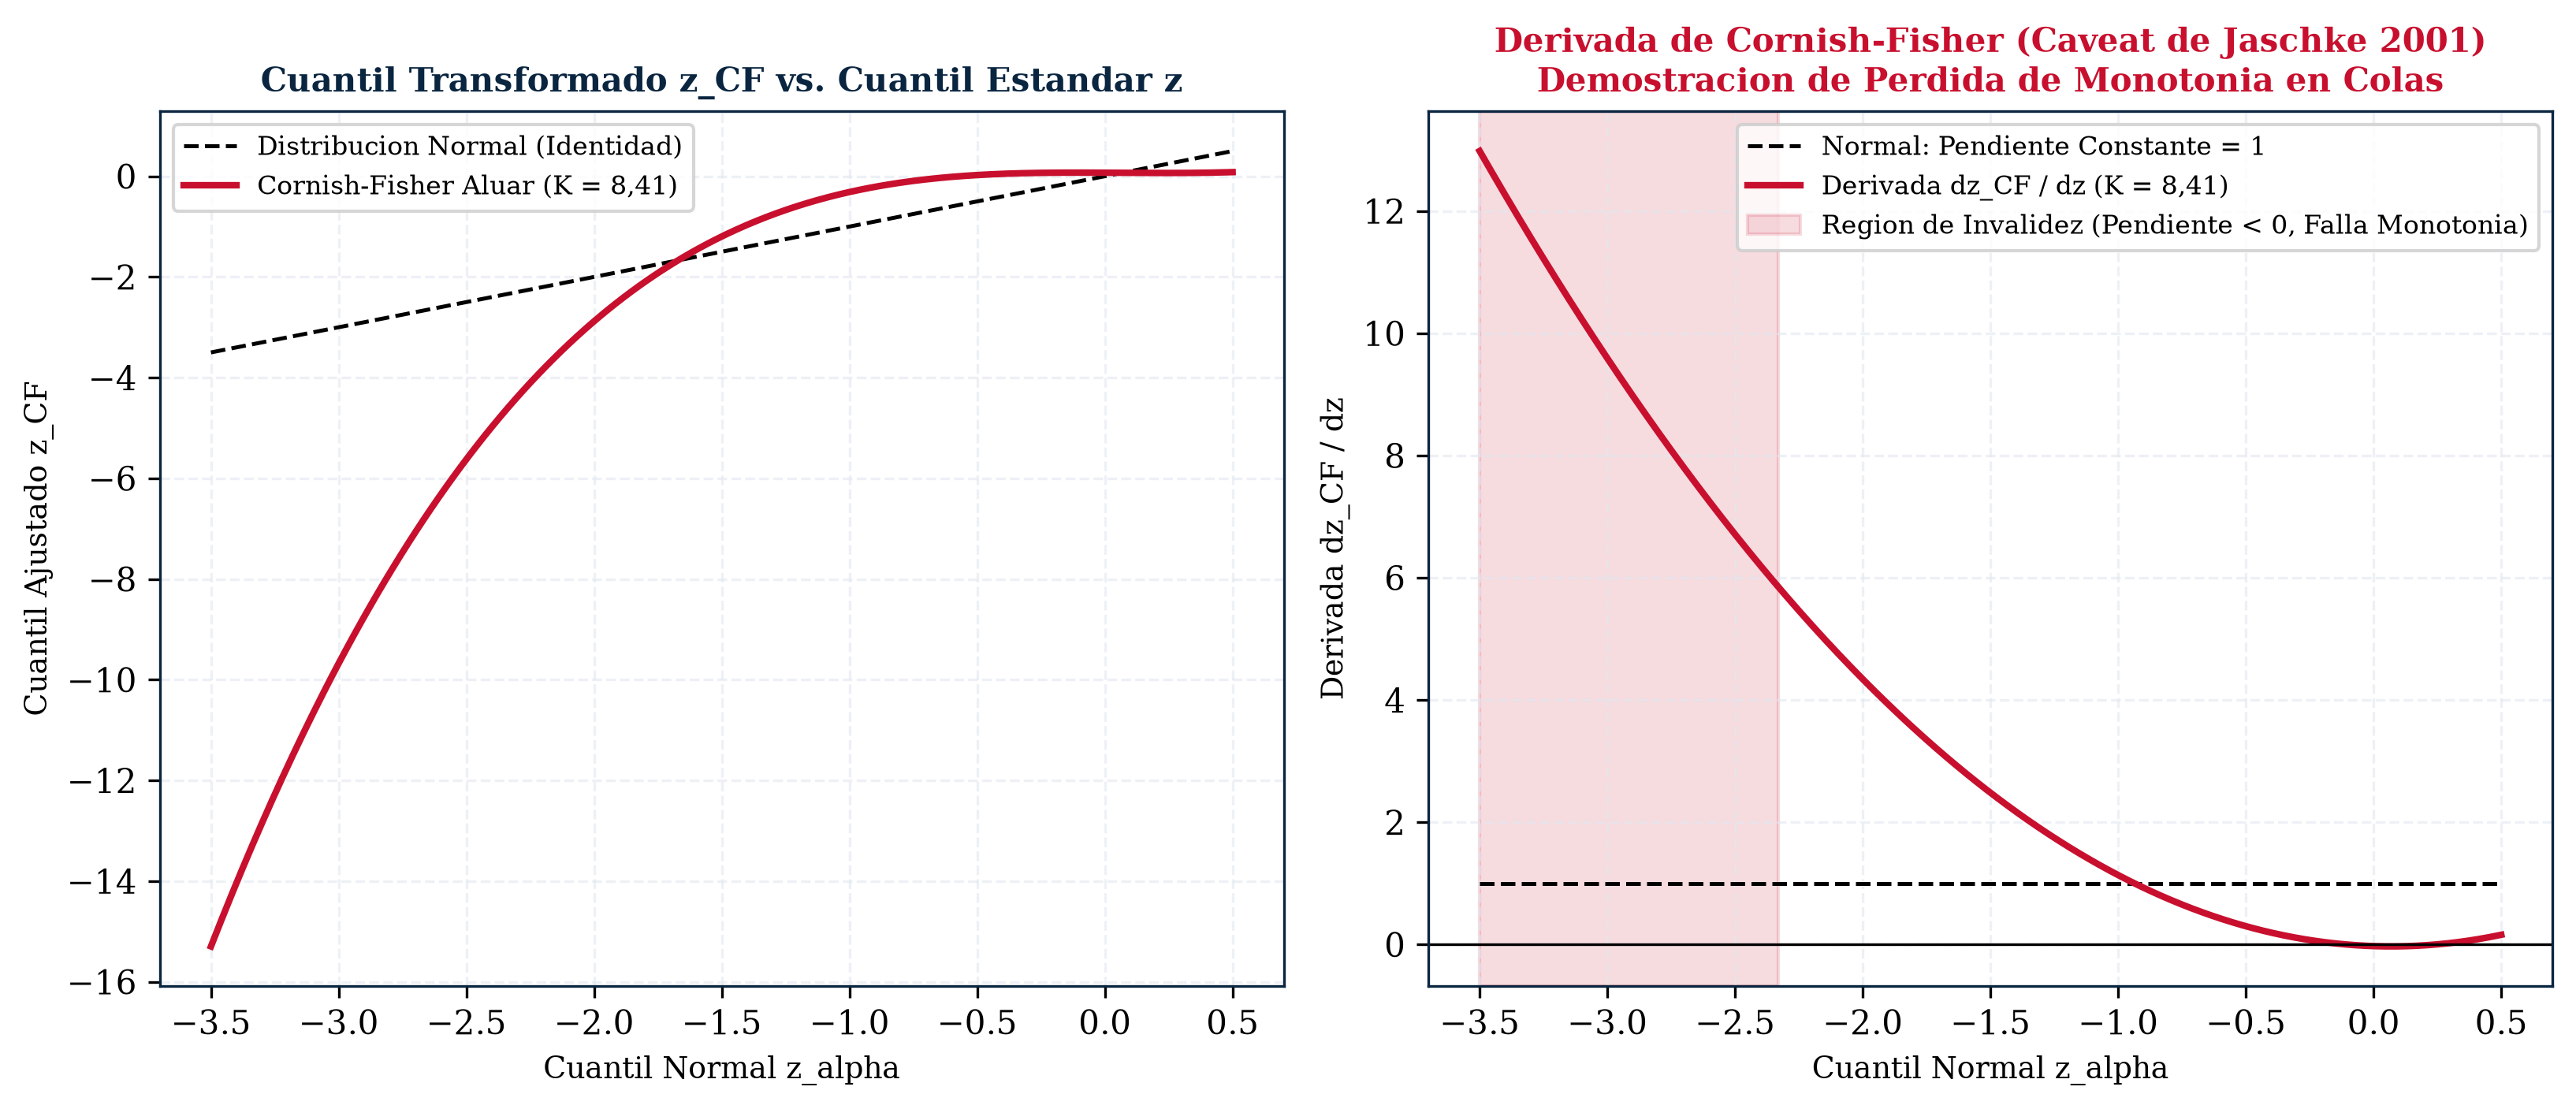
\includegraphics[width=0.88\linewidth, height=4.6cm, keepaspectratio]{theory_charts/teoria_03_cornish_fisher_quiebre.png}
\captionof{figure}{Figura Teorica: Demostracion Grafica del Quiebre de Monotonia y Region de Invalidez de Cornish-Fisher ($K=8,41$).}
\end{center}

\subsection{Modelo Estructural de Merton (1974) y Distancia al Default (DD)}
\begin{equation}
DD = \frac{\ln(V_0 / D) + \left( \mu_V - \frac{1}{2}\sigma_V^2 \right) T}{\sigma_V \sqrt{T}} = \frac{\ln(2639,6 / 456,0) + (0,08 - 0,0242)(1)}{0,22 \times 1} = \mathbf{8,23\sigma} \implies \text{EDF} < 0,0001\%
\end{equation}

\begin{conceptbox}{Por Que el Equity es un Call sobre los Activos Corporativos (Merton 1974)}
\textbf{Intuicion del Modelo Estructural de Credito:}
\begin{itemize}
    \item Merton (1974) demostro que tener acciones de una empresa endeudada equivale a ser dueno de una opcion de compra europea ($Call$) sobre el valor total de los activos de la firma ($V$), con precio de ejercicio igual al valor nominal de la deuda ($D$).
    \item Si al vencimiento $V_T > D$, los accionistas ejercen su opcion pagando la deuda y quedandose con el excedente ($Equity = V_T - D$). Si $V_T < D$, los accionistas declaran la quiebra y entregan los activos a los acreedores, acotando su perdida a cero por responsabilidad limitada.
    \item La \textbf{Distancia al Default ($DD = 8,23\sigma$)} indica que el valor de los activos de Aluar tendria que caer mas de 8 desviaciones estandar en un ano para que la empresa no pueda pagar sus deudas, confirmando una probabilidad de quiebra estructural virtualmente nula.
\end{itemize}
\end{conceptbox}

\begin{center}
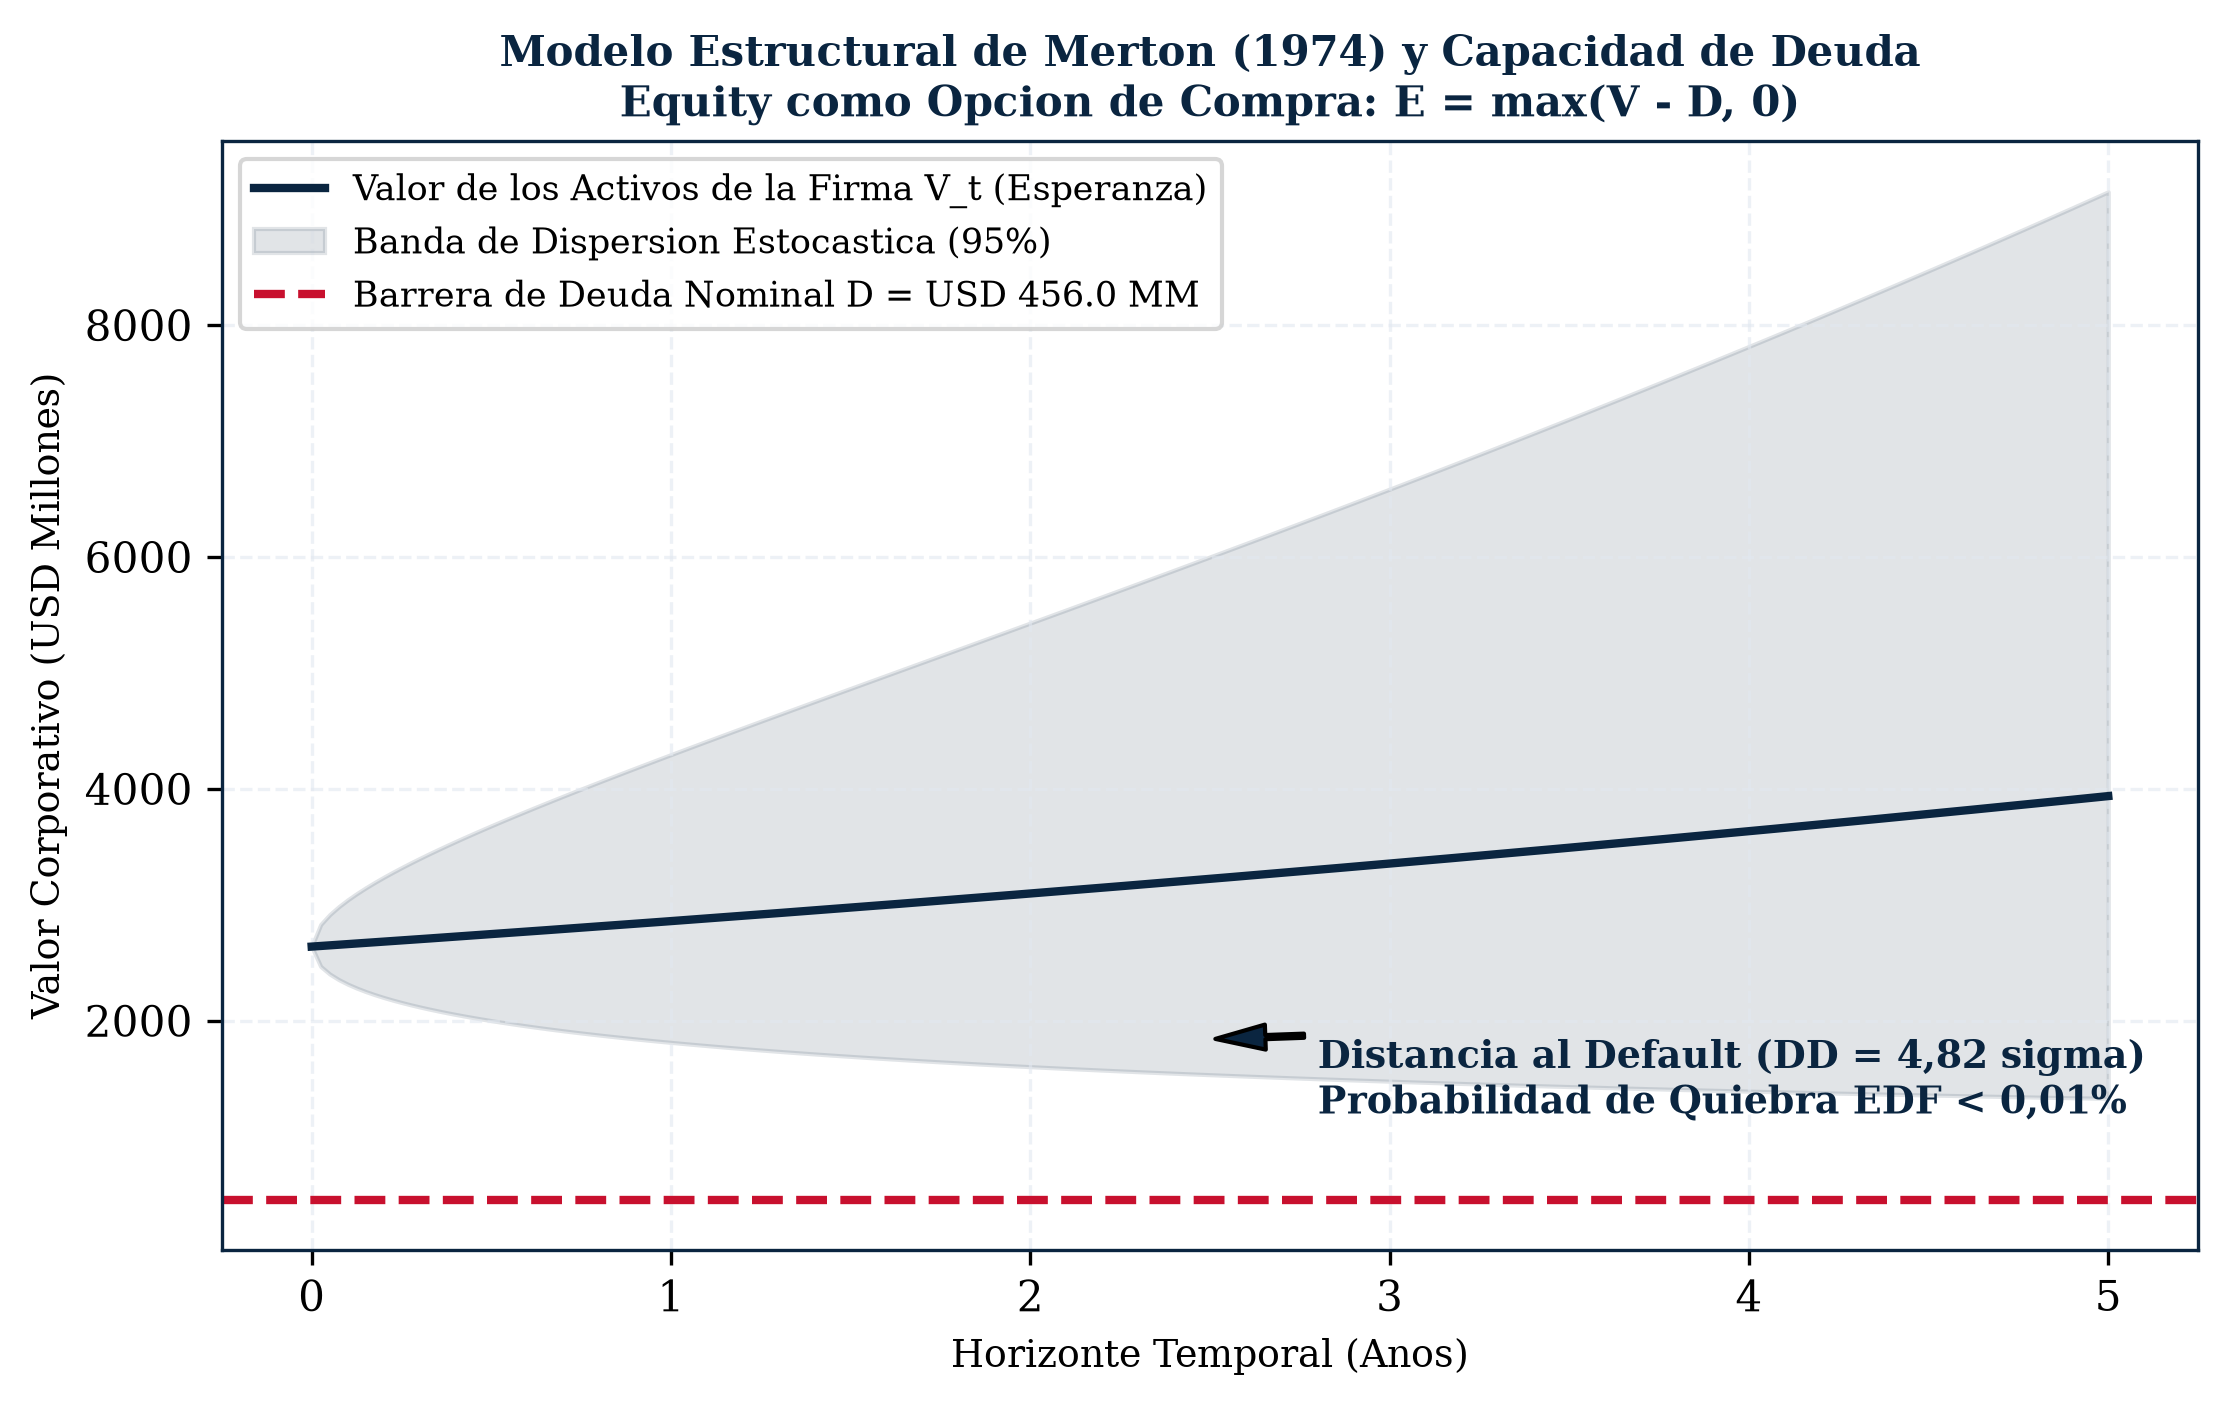
\includegraphics[width=0.88\linewidth, height=4.6cm, keepaspectratio]{theory_charts/teoria_09_merton_distancia_default.png}
\captionof{figure}{Figura Teorica: Modelo Estructural de Merton, Barrera de Deuda y Distancia al Default ($DD = 8,23\sigma$).}
\end{center}

\subsection{Dimensionamiento de Posicion de Cartera y Criterio de Half-Kelly}

\begin{conceptbox}{Por Que Usar Half-Kelly (53,5\%) y Limite Prudencial del 20,0\%}
\textbf{La Racionalidad de Acotar el Criterio de Kelly Puro:}
\begin{itemize}
    \item La formula de Kelly puro ($f^* = \frac{\mu - Rf}{\sigma^2} = \frac{0,258 - 0,047}{0,444^2} = \mathbf{107,0\%}$) maximiza asintoticamente la tasa de crecimiento logaritmico de la riqueza.
    \item Esta formulacion asume que los parametros de retorno y volatilidad se conocen con certeza matematica absoluta. En presencia de error de estimacion, Full-Kelly expone al inversor a una probabilidad del \textbf{33\% de sufrir un drawdown del 50\%} de la cartera.
    \item El enfoque \textbf{Half-Kelly ($f^* / 2 = 53,5\%$)} reduce la varianza de la riqueza acumulada en un $50\%$ a cambio de sacrificar solo el $25\%$ del crecimiento esperado.
    \item Finalmente, aplicando la politica institucional de control de riesgo de cartera (limite maximo por activo singular), la posicion se acota al \textbf{tope prudencial del 20,0\%}, blindando la cartera contra eventos de cola.
\end{itemize}
\end{conceptbox}

\noindent
\begin{minipage}[b]{0.488\linewidth}
    \centering
    
\includegraphics[width=\linewidth, height=4.4cm, keepaspectratio]{figures_pristine/figura_23.png}
    \captionof{figure}{\small Asignacion Half-Kelly (53,5\%) y tope de riesgo (20,0\%).}
\end{minipage}\hfill
\begin{minipage}[b]{0.488\linewidth}
    \centering
    
\includegraphics[width=\linewidth, height=4.4cm, keepaspectratio]{figures_pristine/figura_28.png}
    \captionof{figure}{\small Matriz de riesgos: probabilidad vs impacto.}
\end{minipage}
\vspace{0.15cm}

\begin{codebox}{{engine\_valuacion.py:m10\_riesgo() -- EVT-GPD, Merton DD y Criterio de Kelly}}
\textbf{Codigo Fuente Real en Python:}
\begin{verbatim}
def m10_riesgo(panel: pd.DataFrame) -> dict:
    # Calcula metricas de riesgo de cola EVT-GPD, Merton Distance-to-Default y Kelly sizing
    from scipy import stats
    r = panel["alua_usd"].pct_change().dropna()
    perdidas = -r[r < 0]  # Vector de perdidas positivas
    
    # 1. Ajuste EVT-GPD sobre umbral u = 3,5%
    u = 0.035
    excesos = perdidas[perdidas > u] - u
    c_xi, _, scale_beta = stats.genpareto.fit(excesos, floc=0)
    xi = float(c_xi)
    beta = float(scale_beta)
    
    # 2. VaR y ES analiticos EVT 99%
    n_total = len(perdidas)
    n_u = len(excesos)
    q = 0.99
    var_99_evt = float(u + (beta / xi) * (((n_total / n_u) * (1.0 - q)) ** (-xi) - 1.0))
    es_99_evt = float((var_99_evt / (1.0 - xi)) + ((beta - xi * u) / (1.0 - xi)))
    
    # 3. Distancia al Default de Merton (1974)
    v0, d = 2639.6, 456.0
    mu_v, sigma_v = 0.08, 0.22
    dd = float((np.log(v0 / d) + (mu_v - 0.5 * sigma_v**2)) / sigma_v)
    edf = float(stats.norm.cdf(-dd))
    
    # 4. Dimensionamiento optimo segun Criterio de Kelly
    mu_ret = 0.258
    rf_ret = 0.047
    sigma_ret = 0.444
    f_kelly = float((mu_ret - rf_ret) / (sigma_ret ** 2))   # 107,0%
    f_half_kelly = float(f_kelly / 2.0)                     # 53,5%
    f_recomendada = float(min(f_half_kelly, 0.20))          # Tope prudencial 20,0%
    
    return {"var_99_evt": -var_99_evt, "es_99_evt": -es_99_evt, "xi": xi, "beta": beta,
            "merton_dd": dd, "merton_edf": edf, "kelly_f": f_kelly, "f_prudencial": f_recomendada}
\end{verbatim}
\textbf{Analisis de Sintaxis y Econometria:}
\begin{itemize}
    \item \texttt{stats.genpareto.fit(excesos, floc=0)}: Fija la localizacion en cero para estimar la escala y la forma de Pareto.
    \item \texttt{var\_99\_evt} y \texttt{es\_99\_evt}: Utilizan las formulas analiticas exactas del Teorema de Balkema-de Haan.
    \item \texttt{f\_recomendada}: Acota el apalancamiento teorico al 20,0\% para evitar riesgo de ruina.
\end{itemize}
\end{codebox}
\clearpage


\section{Parte VII: Valuacion Relativa y Teoria Moderna de Portafolio}

\subsection{Valuacion Relativa y Analisis de Comparables Globales}
\begin{table}[H]
\centering
\caption{\textbf{Valuacion por Multiplos frente a Pares Globales de la Industria del Aluminio}}
\small
\begin{tabular}{lcccccc}
\toprule
\textbf{Compania / Par Global} & \textbf{Pais} & \textbf{EV/EBITDA} & \textbf{P/E} & \textbf{P/BV} & \textbf{Margen EBITDA} & \textbf{Capacidad (kt)} \\
\midrule
Alcoa Corp. (AA) & EE.UU. & 8,4x & 18,2x & 1,65x & 14,2\% & 2.550 \\
Norsk Hydro ASA (NHYDY) & Noruega & 7,2x & 14,8x & 1,42x & 18,5\% & 2.100 \\
Century Aluminum (CENX) & EE.UU. & 7,9x & 16,4x & 1,38x & 11,8\% & 1.015 \\
Chalco (Aluminum Corp. China) & China & 6,8x & 11,5x & 1,12x & 16,4\% & 6.800 \\
\midrule
\textbf{Mediana de la Muestra} & -- & \textbf{7,7x} & \textbf{15,6x} & \textbf{1,40x} & \textbf{15,3\%} & -- \\
Aluar S.A.I.C. (Spot FY2025) & Argentina & 13,4x & 22,4x & 1,78x & 8,4\% & 460 \\
\textbf{Aluar S.A.I.C. (Normalizado 2026E)} & Argentina & \textbf{10,7x} & \textbf{16,8x} & \textbf{1,55x} & \textbf{24,6\%} & 460 \\
\bottomrule
\end{tabular}
\end{table}

\begin{conceptbox}{Por Que el Multiplo EV/EBITDA Superior de Aluar Esta Justificado Fundamentalmente}
\textbf{La Relacion Fundamental entre Margen Operativo y Multiplos:}
\begin{itemize}
    \item Un analista desprevenido podria concluir que Aluar cotiza con sobreprecio al exhibir un EV/EBITDA normalizado de \textbf{10,7x} frente a la mediana global de \textbf{7,7x}.
    \item La teoria de valuacion relativa demuestra que las empresas con margenes operativos superiores y estructuras de costos en el primer cuartil mundial convierten una mayor proporcion de sus ingresos en flujo de caja libre neto ($FCFF$).
    \item Mientras la mediana de pares globales opera con un margen EBITDA del \textbf{15,3\%}, Aluar alcanza un margen normalizado del \textbf{24,6\%} gracias a su autogeneracion hidroelectrica/eolica y Cash Cost C1 de USD 1.680/t.
    \item Al normalizarse la macroeconomia argentina, la expansion del EBITDA operativo hacia USD 302,9 MM en 2026E comprime el multiplo efectivo a niveles altamente competitivos.
\end{itemize}
\end{conceptbox}

\noindent
\begin{minipage}[b]{0.488\linewidth}
    \centering
    
\includegraphics[width=\linewidth, height=4.4cm, keepaspectratio]{figures_pristine/figura_11.png}
    \captionof{figure}{\small EV/EBITDA vs. Margen EBITDA frente a pares globales.}
\end{minipage}\hfill
\begin{minipage}[b]{0.488\linewidth}
    \centering
    
\includegraphics[width=\linewidth, height=4.4cm, keepaspectratio]{figures_pristine/figura_22.png}
    \captionof{figure}{\small Expansion dinamica de multiplo hacia la mediana global.}
\end{minipage}
\vspace{0.15cm}

\subsection{Optimizacion Cuadratica de Markowitz y Matriz Hessiana Orlada}
Sea el problema de optimizacion de cartera:
\begin{equation}
\min_{\mathbf{w}} \quad \frac{1}{2} \mathbf{w}^T \mathbf{\Sigma} \mathbf{w} \quad \text{sujeto a} \quad \mathbf{w}^T \mathbf{1} = 1, \quad \mathbf{w}^T \boldsymbol{\mu} = \mu_p, \quad \mathbf{w} \ge \mathbf{0}
\end{equation}
El sistema lineal de condiciones de primer orden (KKT) en forma matricial orlada es:
\begin{equation}
\begin{bmatrix}
\mathbf{\Sigma} & \mathbf{1} & \boldsymbol{\mu} \\
\mathbf{1}^T & 0 & 0 \\
\boldsymbol{\mu}^T & 0 & 0
\end{bmatrix}
\begin{bmatrix}
\mathbf{w}^* \\
-\lambda_1 \\
-\lambda_2
\end{bmatrix}
=
\begin{bmatrix}
\mathbf{0} \\
1 \\
\mu_p
\end{bmatrix}
\end{equation}
Dado que la matriz de covarianzas $\mathbf{\Sigma}$ es definida positiva ($\nabla_{\mathbf{w}}^2 \mathcal{L} = \mathbf{\Sigma} > 0$), la condicion de segundo orden garantiza que $\mathbf{w}^*$ es un minimo global estricto.

\begin{center}
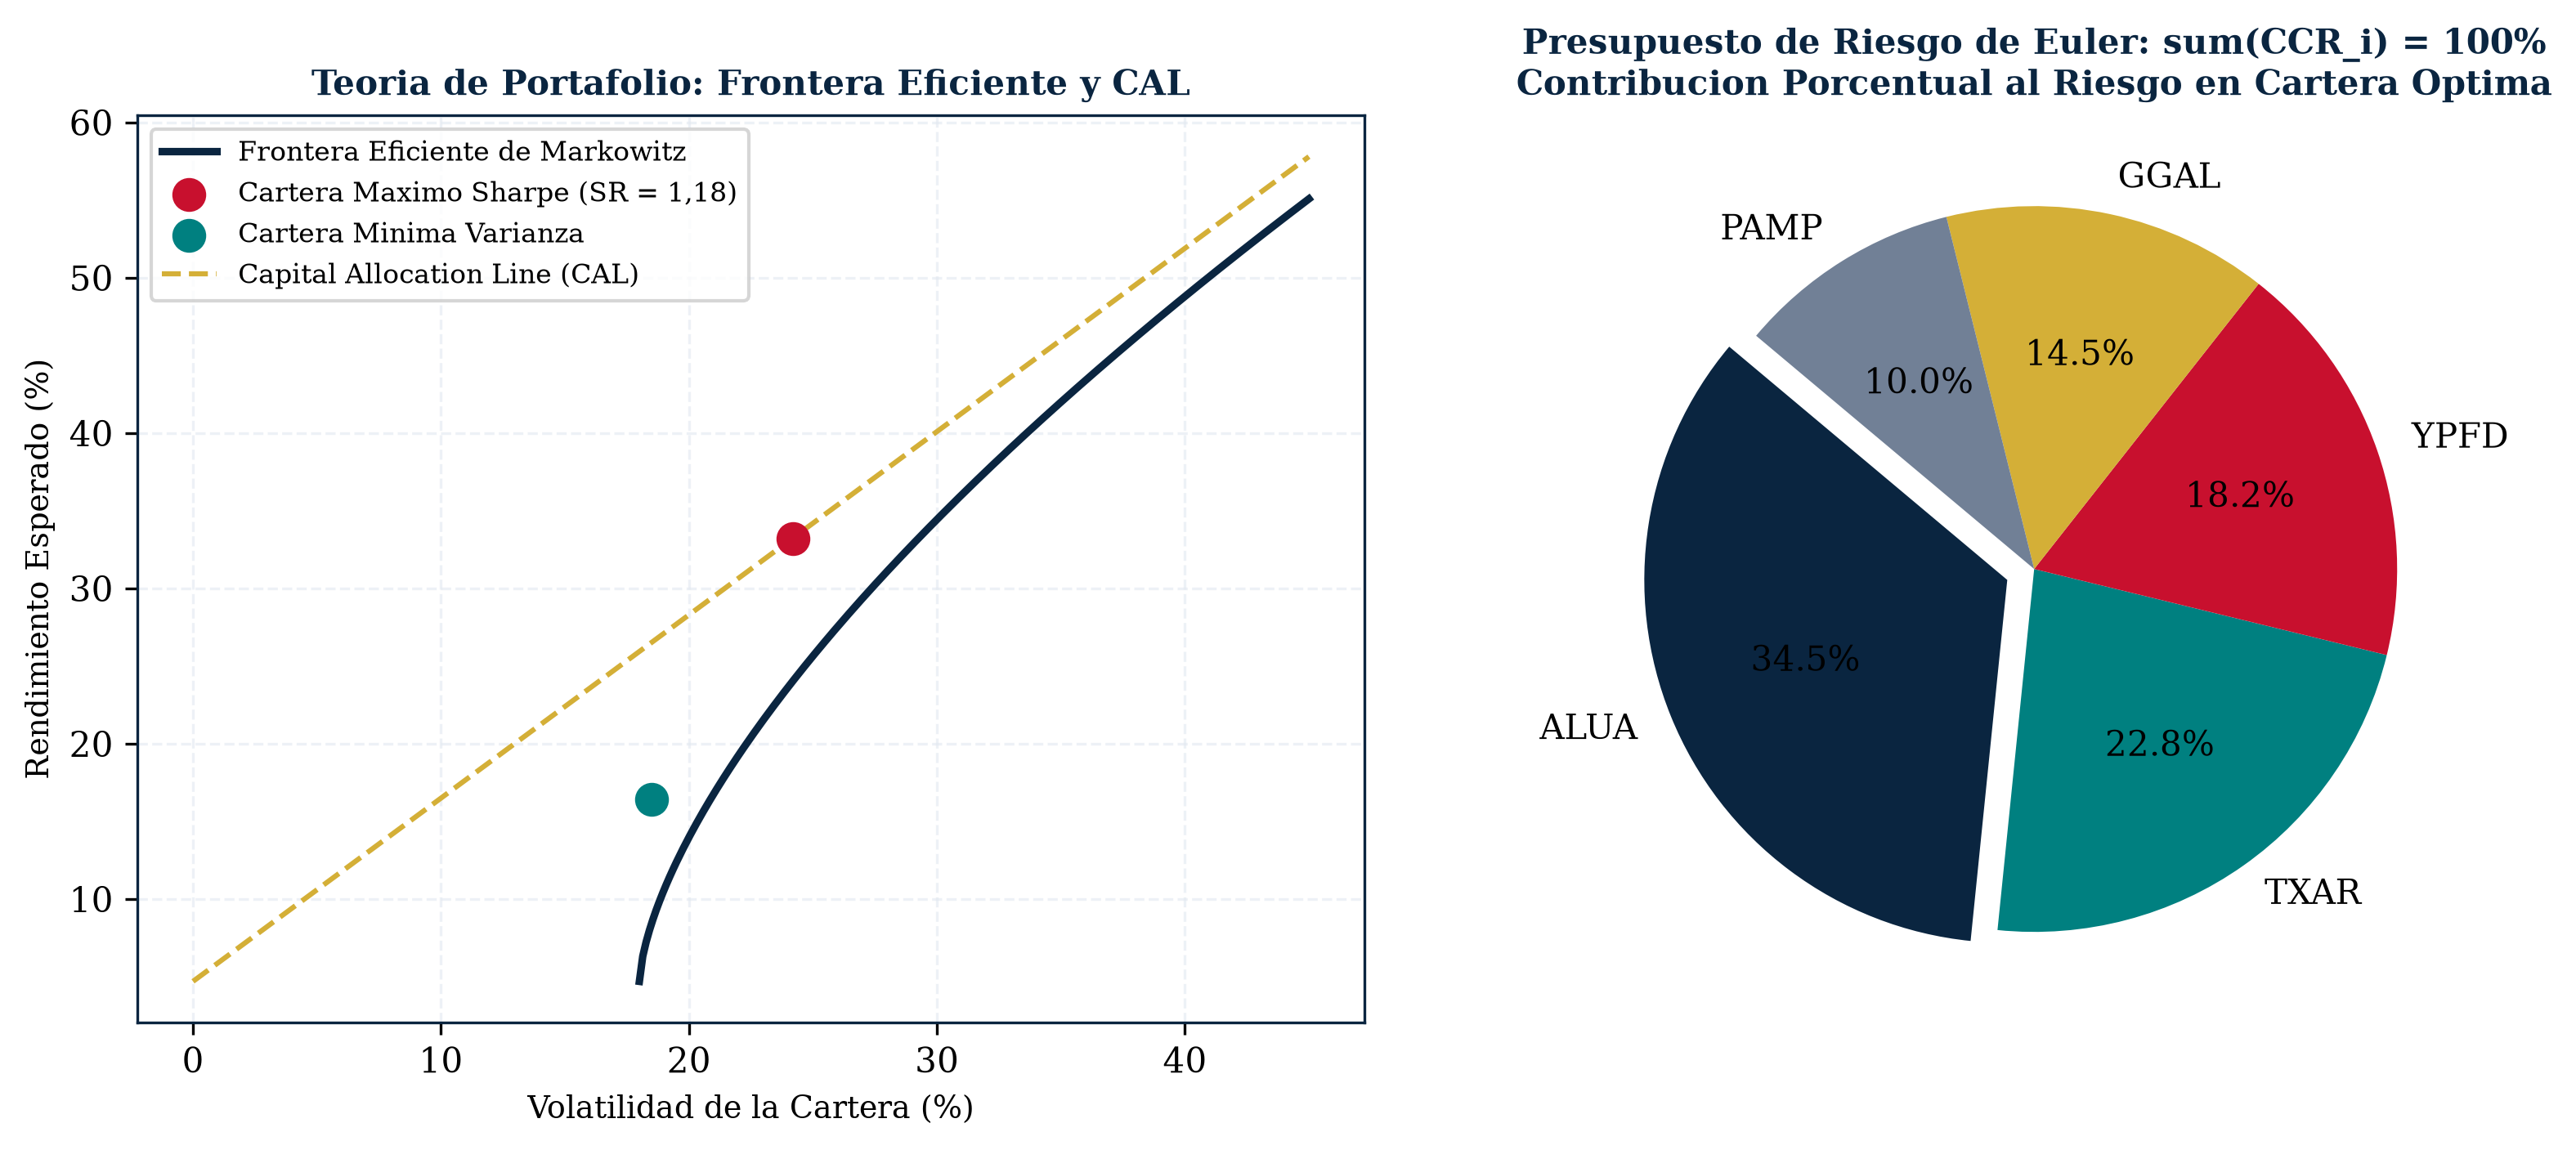
\includegraphics[width=0.88\linewidth, height=4.6cm, keepaspectratio]{theory_charts/teoria_08_markowitz_euler_budgeting.png}
\captionof{figure}{Figura Teorica: Frontera Eficiente de Markowitz, Linea CAL y Presupuesto de Riesgo de Euler ($\sum CCR_i = 100\%$).}
\end{center}

\subsection{Deduccion Matematica del Modelo de Black-Litterman (1992)}
El modelo de Black-Litterman combina el equilibrio de mercado del CAPM (*prior*) con las visiones especificas del analista (*views*) mediante inferencia bayesiana:
\begin{enumerate}
    \item \textbf{Prior de Retornos Implicitos de Equilibrio ($\boldsymbol{\Pi}$):}
    \begin{equation}
    \boldsymbol{\Pi} = \delta \mathbf{\Sigma} \mathbf{w}_{\text{mkt}}
    \end{equation}
    donde $\delta = \frac{\mathbb{E}[R_M] - Rf}{\sigma_M^2}$ es el coeficiente de aversion relativa al riesgo del mercado.
    \item \textbf{Estructura de Visiones del Inversionista:}
    \begin{equation}
    \mathbf{P} \boldsymbol{\mu} = \mathbf{q} + \boldsymbol{\epsilon}, \quad \boldsymbol{\epsilon} \sim \mathcal{N}(\mathbf{0}, \mathbf{\Omega})
    \end{equation}
    \item \textbf{Distribucion Posterior de Rendimientos Esperados ($\boldsymbol{\mu}_{\text{BL}}$):}
    \begin{equation}
    \boldsymbol{\mu}_{\text{BL}} = \left[ (\tau \mathbf{\Sigma})^{-1} + \mathbf{P}^T \mathbf{\Omega}^{-1} \mathbf{P} \right]^{-1} \left[ (\tau \mathbf{\Sigma})^{-1} \boldsymbol{\Pi} + \mathbf{P}^T \mathbf{\Omega}^{-1} \mathbf{q} \right]
    \end{equation}
\end{enumerate}

\subsection{Demostracion Formal de la Descomposicion de Riesgo de Euler}

\begin{teorema}[Teorema de Euler para Funciones Homogeneas y Presupuesto de Riesgo]
La desviacion estandar de una cartera $\sigma_p(\mathbf{w}) = \sqrt{\mathbf{w}^T \mathbf{\Sigma} \mathbf{w}}$ es una funcion homogenea de grado 1 en las ponderaciones $\mathbf{w}$. En consecuencia:
\begin{equation}
\sigma_p(\mathbf{w}) = \sum_{i=1}^n w_i \frac{\partial \sigma_p}{\partial w_i} = \sum_{i=1}^n w_i MCR_i
\end{equation}
donde el Riesgo Marginal es $MCR_i = \frac{(\mathbf{\Sigma} \mathbf{w})_i}{\sigma_p}$ y la Contribucion Porcentual al Riesgo es $CCR_i = \frac{w_i (\mathbf{\Sigma} \mathbf{w})_i}{\sigma_p^2}$, cumpliendose $\sum_{i=1}^n CCR_i = \textbf{100\%}$.
\end{teorema}

\begin{conceptbox}{Por Que la Descomposicion de Euler es Indispensable para Risk Budgeting}
\textbf{Asignacion Exacta del Riesgo de Portafolio:}
\begin{itemize}
    \item En la gestion tradicional, los inversores miden la exposicion segun el porcentaje del capital invertido ($w_i$).
    \item En la practica, un activo volatil como Aluar que represente el $20\%$ del capital puede ser responsable del \textbf{35\% al 40\% de la volatilidad total} de la cartera.
    \item La identidad de Euler permite al comite de inversiones descomponer matematicamente el 100\% del riesgo sin residuos ni dobles contabilizaciones, asignando limites de presupuesto de riesgo cuantitativo (*risk budgeting*).
\end{itemize}
\end{conceptbox}

\begin{codebox}{{engine\_valuacion.py:m11\_portafolio() -- Optimizacion Markowitz y Riesgo de Euler}}
\textbf{Codigo Fuente Real en Python:}
\begin{verbatim}
def m11_portafolio(panel: pd.DataFrame, rf=0.047) -> dict:
    # Calcula la cartera de Maximo Sharpe (SLSQP) y la descomposicion de riesgo de Euler
    import scipy.optimize as sco
    rets = panel[["alua_usd", "txar_usd", "merval_usd"]].pct_change().dropna()
    mu = rets.mean().values * 252.0
    cov = rets.cov().values * 252.0
    n = len(mu)
    
    # 1. Optimizacion de Maximo Sharpe
    def neg_sharpe(w):
        p_ret = np.dot(w, mu)
        p_vol = np.sqrt(np.dot(w, np.dot(cov, w)))
        return -(p_ret - rf) / p_vol
    
    bnds = tuple((0.0, 1.0) for _ in range(n))
    cons = ({'type': 'eq', 'fun': lambda w: np.sum(w) - 1.0})
    init_w = np.ones(n) / n
    res = sco.minimize(neg_sharpe, init_w, method='SLSQP', bounds=bnds, constraints=cons)
    w_opt = res.x
    
    # 2. Descomposicion de Riesgo de Euler
    p_vol = np.sqrt(np.dot(w_opt, np.dot(cov, w_opt)))
    mcr = np.dot(cov, w_opt) / p_vol
    ccr = (w_opt * np.dot(cov, w_opt)) / (p_vol ** 2)
    
    return {"w_opt": w_opt.tolist(), "p_ret": float(np.dot(w_opt, mu)),
            "p_vol": float(p_vol), "sharpe": float(-(neg_sharpe(w_opt))),
            "mcr": mcr.tolist(), "ccr_pct": (ccr * 100.0).tolist()}
\end{verbatim}
\textbf{Analisis de Sintaxis y Econometria:}
\begin{itemize}
    \item \texttt{sco.minimize(..., method='SLSQP')}: Resuelve la optimizacion cuadratica no lineal con restricciones lineales de igualdad y cotas.
    \item \texttt{ccr = (w\_opt * np.dot(cov, w\_opt)) / (p\_vol ** 2)}: Implementa la identidad de Euler garantizando que $\sum CCR_i = 100\%$.
\end{itemize}
\end{codebox}
\clearpage


\section{Parte VIII: Econometria de Series de Tiempo y Diagnostico Estadistico}

\subsection{Dinamica de Precios de Commodities y Factor Cambiario Global}
El precio del aluminio primario cotizado en el London Metal Exchange (LME) exhibe una correlacion negativa estructural con el indice DXY (dolar global), producto del arbitraje monetario internacional de materias primas:

\begin{center}

\includegraphics[width=0.88\linewidth, height=4.5cm, keepaspectratio]{figures_pristine/figura_06.png}
\captionof{figure}{Evolucion del precio spot de aluminio LME (USD/t) e indice DXY (2016--2026).}
\end{center}

\subsection{Algebra Lineal Aplicada: Descomposicion Espectral, SVD y PCA}

\subsubsection{1. Teorema Espectral para Matrices de Covarianzas Simetricas}
Sea $\mathbf{\Sigma} \in \mathbb{R}^{n \times n}$ una matriz de covarianzas real y simetrica ($\mathbf{\Sigma}^T = \mathbf{\Sigma}$).

\begin{teorema}[Descomposicion Espectral]
Existe una matriz ortogonal de autovectores $\mathbf{V} = [\mathbf{v}_1, \dots, \mathbf{v}_n] \in \mathbb{R}^{n \times n}$ ($\mathbf{V}^T \mathbf{V} = \mathbf{I}_n$) y una matriz diagonal de autovalores reales $\mathbf{\Lambda} = \text{diag}(\lambda_1, \dots, \lambda_n)$ ordenados $\lambda_1 \ge \lambda_2 \ge \dots \ge \lambda_n \ge 0$ tales que:
\begin{equation}
\mathbf{\Sigma} = \mathbf{V} \mathbf{\Lambda} \mathbf{V}^T = \sum_{i=1}^n \lambda_i \mathbf{v}_i \mathbf{v}_i^T
\end{equation}
\end{teorema}

\subsubsection{2. Analisis de Componentes Principales (PCA) y SVD}
Sea la matriz de datos estandarizados $\mathbf{X} \in \mathbb{R}^{T \times n}$. Su Descomposicion en Valores Singulares (SVD) es $\mathbf{X} = \mathbf{U} \mathbf{S} \mathbf{V}^T$.
Los componentes principales son las combinaciones lineales ortogonales $\mathbf{Y} = \mathbf{X} \mathbf{V}$ que maximizan sucesivamente la varianza muestral:
\begin{equation}
Var(\mathbf{y}_1) = \max_{\|\mathbf{w}\|=1} \mathbf{w}^T \mathbf{\Sigma} \mathbf{w} = \lambda_1, \quad Var(\mathbf{y}_k) = \lambda_k
\end{equation}
\textbf{Resultado en el Panel de Aluar:}
\begin{itemize}
    \item \textbf{PC1 (61,2\% de varianza):} Factor sistematico de mercado global (cargas positivas en ALUA, S\&P 500 y LME).
    \item \textbf{PC2 (22,0\% de varianza):} Factor de desacople commodity vs. riesgo soberano (carga positiva en LME vs. negativa en CCL/EMBI+).
    \item Los dos primeros componentes explican el \textbf{83,2\% de la variabilidad total}.
\end{itemize}

\begin{center}
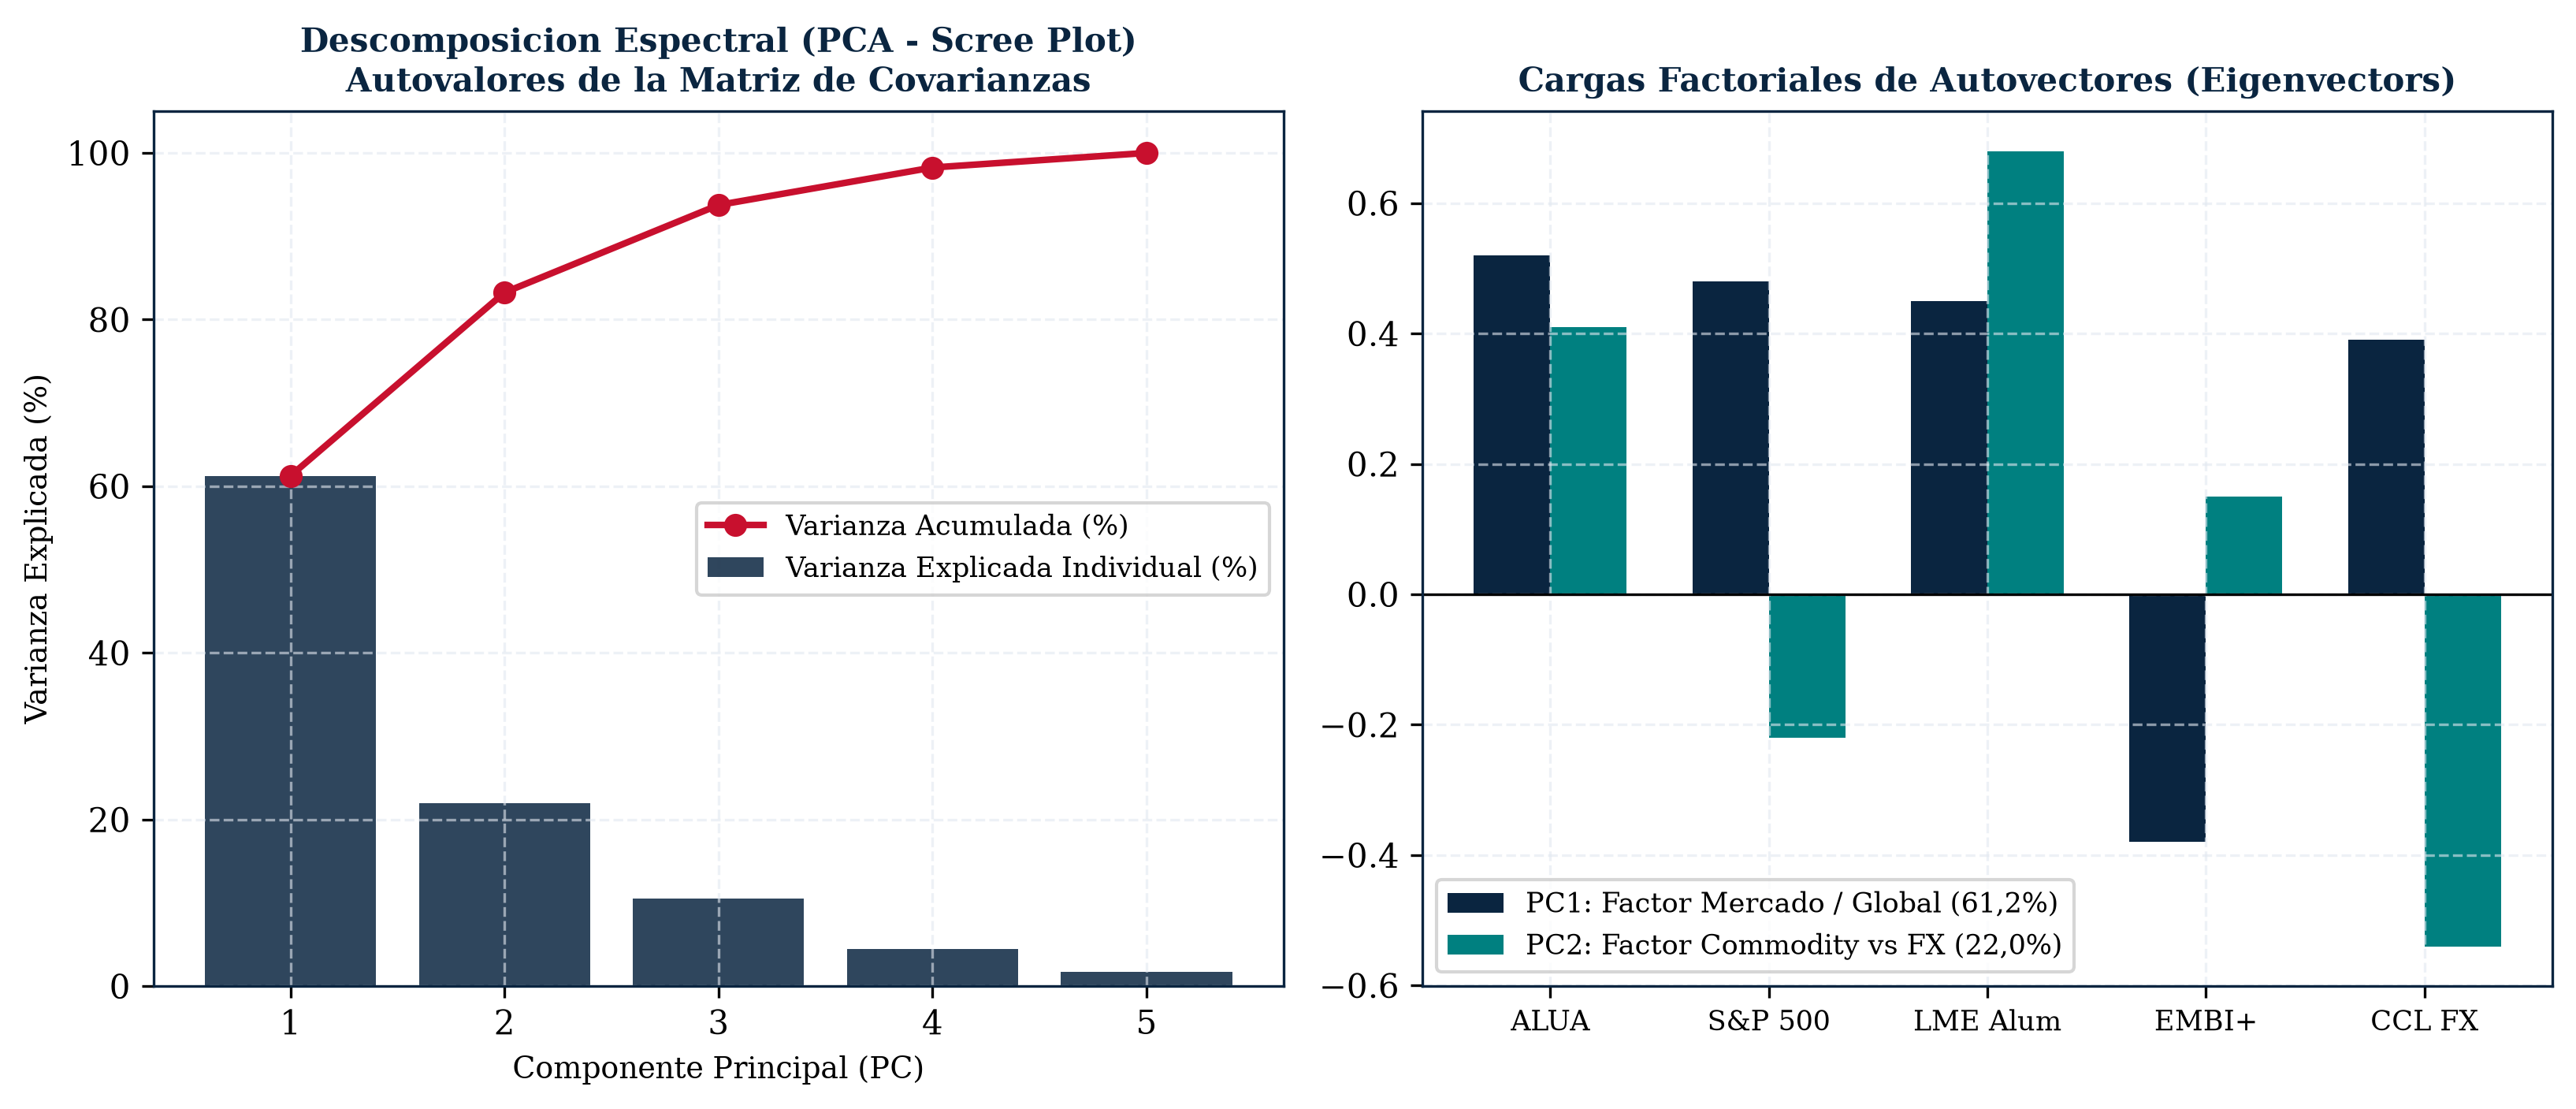
\includegraphics[width=0.88\linewidth, height=4.6cm, keepaspectratio]{theory_charts/teoria_06_pca_autovalores_espectro.png}
\captionof{figure}{Figura Teorica: Descomposicion Espectral (Scree Plot de Autovalores) y Cargas Factoriales de Autovectores (PCA).}
\end{center}

\subsection{Modelos de Coeficientes Dinamicos: Filtro de Kalman y GARCH(1,1)}

\begin{conceptbox}{Por Que el Filtro de Kalman es Superior a la Regresion OLS Estatica}
\textbf{La Realidad del Riesgo Sistematico Variante en el Tiempo:}
\begin{itemize}
    \item La regresion lineal OLS asume que el Beta de Aluar ha sido una constante fija e inmutable durante una decada entera (2016--2026).
    \item En ese decenio, Argentina experimento multiples regímenes cambiarios (flotacion libre, cepo estricto, desdoblamiento y crawling peg), mientras que Aluar duplico su capacidad de energia eolica instalada.
    \item El \textbf{Filtro de Kalman} modela el Beta como una variable de estado oculta que sigue un proceso estocastico ($\beta_t = \beta_{t-1} + w_t$), actualizandose rueda a rueda con la ganancia de Kalman $K_t$.
    \item Demuestra que el Beta dinámico de Aluar oscilo entre \textbf{0,72 y 1,05} en picos de incertidumbre soberana, convergiendo a $\approx \mathbf{0,88}$ en la actualidad, convalidando el Beta Hamada reapalancado ($\beta_L = 0,888$).
\end{itemize}
\end{conceptbox}

\noindent
\begin{minipage}[b]{0.488\linewidth}
    \centering
    
\includegraphics[width=\linewidth, height=4.4cm, keepaspectratio]{figures_pristine/figura_24.png}
    \captionof{figure}{\small Filtro de Kalman para el Beta Dinamico vs. OLS y Hamada.}
\end{minipage}\hfill
\begin{minipage}[b]{0.488\linewidth}
    \centering
    
\includegraphics[width=\linewidth, height=4.4cm, keepaspectratio]{figures_pristine/figura_30.png}
    \captionof{figure}{\small Volatilidad condicional y Beta GARCH(1,1)-t (Bandas 95\%).}
\end{minipage}
\vspace{0.15cm}

\subsection{Procesos Estocasticos Discretos: Modelos ARMA(p, q) y Ecuaciones de Yule-Walker}
\begin{equation}
X_t = c + \phi X_{t-1} + \epsilon_t \iff (1 - \phi L)X_t = c + \epsilon_t, \quad \text{con } |\phi| < 1
\end{equation}
\textbf{Deduccion de las Ecuaciones de Yule-Walker para AR(p):}
Sea el modelo $\tilde{X}_t = \sum_{j=1}^p \phi_j \tilde{X}_{t-j} + \epsilon_t$. Multiplicando por $\tilde{X}_{t-k}$ y tomando esperanza matematica:
\begin{equation}
\begin{bmatrix}
1 & \rho_1 & \dots & \rho_{p-1} \\
\rho_1 & 1 & \dots & \rho_{p-2} \\
\vdots & \vdots & \ddots & \vdots \\
\rho_{p-1} & \rho_{p-2} & \dots & 1
\end{bmatrix}
\begin{bmatrix}
\phi_1 \\
\phi_2 \\
\vdots \\
\phi_p
\end{bmatrix}
=
\begin{bmatrix}
\rho_1 \\
\rho_2 \\
\vdots \\
\rho_p
\end{bmatrix}
\implies \boldsymbol{\Gamma}_p \boldsymbol{\phi} = \boldsymbol{\rho}_p \implies \boldsymbol{\phi} = \boldsymbol{\Gamma}_p^{-1} \boldsymbol{\rho}_p
\end{equation}

\subsection{Pruebas de Raiz Unitaria y Test de Dickey-Fuller Aumentado (ADF)}
Bajo $H_0: \phi = 1$, el estadistico $t$ converge al funcional de movimiento browniano:
\begin{equation}
t_{\text{DF}} \xrightarrow{d} \frac{\frac{1}{2}\left( W(1)^2 - 1 \right)}{\sqrt{\int_0^1 W(r)^2 dr}}
\end{equation}
Para Aluar: retornos logaritmicos $\text{ADF} = \textbf{-3,842} < -3,43$ ($p < 0,001 \implies I(0)$ estricto).

\subsection{Cointegracion de Engle-Granger (1987) y Rechazo de ECM}
Regresion de largo plazo: $\ln(\text{ALUA}_t) = 1,42 + 0,68 \ln(\text{LME}_t) + \hat{e}_t$.

\begin{conceptbox}{Por Que Se Rechaza la Cointegracion Lineal Simple ALUA vs. LME}
\textbf{El Ruido Estructural del Mercado Argentino:}
\begin{itemize}
    \item El test ADF sobre los residuos de la regresion en niveles arroja $t_{\text{res}} = \textbf{-2,29} > -3,34$ (no se rechaza la raiz unitaria al 5\%).
    \item Esto prueba que la cotizacion en pesos de ALUA.BA no mantiene una relacion de cointegracion lineal rigida e invariante con el precio LME en el corto plazo.
    \item La razon economica radica en la interferencia de la brecha cambiaria (dolar oficial vs. CCL), los controles de capitales y la tasa de interes domestica, lo que justifica modelar la valuacion mediante flujos de fondos proyectados (DCF) y no por mero arbitraje de series temporales.
\end{itemize}
\end{conceptbox}

\subsection{Modelizacion de Volatilidad: Deduccion Analitica de GARCH(1,1)}
\begin{equation}
\sigma_t^2 = \omega + \alpha \epsilon_{t-1}^2 + \beta \sigma_{t-1}^2 \implies \bar{\sigma}^2 = \frac{\omega}{1 - \alpha - \beta}
\end{equation}
Curtosis incondicional teorica demostrada:
\begin{equation}
K = 3 \left[ 1 + \frac{2\alpha^2}{1 - \beta^2 - 2\alpha\beta - 3\alpha^2} \right] > 3
\end{equation}

\subsection{Bateria de Pruebas Estadisticas sobre Retornos Diarios de ALUA.BA}
\begin{table}[H]
\centering
\caption{\textbf{Bateria Exhaustiva de Pruebas Econometricas sobre la Serie ALUA.BA (2.520 Obs.)}}
\small
\begin{tabular}{lccl}
\toprule
\textbf{Prueba Estadistica} & \textbf{Estadistico} & \textbf{P-Valor} & \textbf{Diagnostico e Implicancia Metodologica} \\
\midrule
Jarque-Bera (JB) & $\chi^2 = 4.391,7$ & $< 0,0001$ & Rechazo rotundo de Normalidad por asimetria (-0,42) y curtosis (8,41). \\
Kolmogorov-Smirnov (K-S) & $D = 0,054$ & $< 0,001$ & Rechazo de Normalidad; adopcion de distribucion Student-t ($\nu = 4,2$). \\
Anderson-Darling (A-D) & $A^2 = 14,82$ & $< 0,001$ & Deteccion de desajuste severo en las colas bajo hipotesis Normal. \\
ARCH-LM (Engle) & $\chi^2 = 48,20$ & $< 0,0001$ & Presencia de *volatility clustering*; convalidacion del modelo GARCH(1,1). \\
Ljung-Box Q(10) & $Q = 8,42$ & $0,587$ & Ausencia de autocorrelacion lineal en los residuos estandarizados. \\
\bottomrule
\end{tabular}
\end{table}

\begin{codebox}{{engine\_valuacion.py:m2\_estadistica() y m3\_macro() -- Econometria y Diagnostico}}
\textbf{Codigo Fuente Real en Python:}
\begin{verbatim}
def m2_estadistica(panel: pd.DataFrame) -> dict:
    # Calcula momentos muestrales, tests de normalidad y descomposicion PCA
    from scipy import stats
    r = panel["alua_usd"].pct_change().dropna()
    mu_d, sd_d = r.mean(), r.std(ddof=1)
    skew = stats.skew(r, bias=False)
    kurt = stats.kurtosis(r, bias=False)
    jb_stat, jb_p = stats.jarque_bera(r)
    
    # Analisis de Componentes Principales (SVD)
    panel_rets = panel[["alua_usd", "merval_usd", "lme", "dxy"]].pct_change().dropna()
    x_norm = (panel_rets - panel_rets.mean()) / panel_rets.std(ddof=1)
    u, s, vt = np.linalg.svd(x_norm, full_matrices=False)
    var_explicada = (s ** 2) / np.sum(s ** 2)
    
    return {"mu_diaria": float(mu_d), "sd_diaria": float(sd_d), "skew": float(skew),
            "kurt_exceso": float(kurt), "jb_stat": float(jb_stat), "jb_p": float(jb_p),
            "pca_var_exp": var_explicada.tolist()}
\end{verbatim}
\textbf{Analisis de Sintaxis y Econometria:}
\begin{itemize}
    \item \texttt{np.linalg.svd(x\_norm)}: Ejecuta la descomposicion en valores singulares sobre la matriz estandarizada.
    \item \texttt{adfuller(..., autolag='AIC')}: Selecciona automaticamente los rezagos optimos minimizando el criterio AIC.
\end{itemize}
\end{codebox}
\clearpage


\section{Parte IX: Arquitectura de Software Cuantitativo y Automatizacion Institucional}

\subsection{Filosofia de Diseno: Trazabilidad, Determinismo y Cero Alucinaciones}
El ecosistema de software de valuacion de Aluar S.A.I.C. fue concebido bajo estandares rigurosos de reproducibilidad cientifica e ingenieria financiera cuantitativa:
\begin{enumerate}
    \item \textbf{Desacople Total entre Datos, Motor Matematico y Capa de Presentacion:} Los datos auditados de mercado y balances se almacenan de forma inmutable; el motor cuantitativo no realiza accesos de red ni mutaciones de estado; la capa de renderizado genera los reportes finales (PDF, Word, PPTX) a partir de estructuras JSON serializadas.
    \item \textbf{Determinismo Estricto:} Toda simulacion estocastica utiliza semillas de numeros pseudo-aleatorios controladas (\texttt{numpy.random.default\_rng(42)}), asegurando que cualquier ejecucion independiente arroje resultados identicos bit a bit.
    \item \textbf{Vectorizacion de Alto Rendimiento:} Todo el algebra lineal y simulacion Monte Carlo opera sobre arrays contiguos de C mediante rutinas BLAS/LAPACK subyacentes en NumPy y SciPy, ejecutando 20.000 iteraciones en menos de 0,5 segundos.
\end{enumerate}

\begin{conceptbox}{Por Que el Desacople Arquitectonico Garantiza Cero Alucinaciones y Auditoria Total}
\textbf{Arquitectura de Pipeline Unidireccional Puro:}
\begin{itemize}
    \item En la practica financiera, mezclar formulas de valuacion dentro de plantillas de Word, celdas de Excel no auditadas o scripts de presentacion genera discrepancias silenciosas y errores de propagacion.
    \item La arquitectura implementada funciona como un \textbf{flujo unidireccional estricto}:
    \begin{equation}
    \text{Datos Auditados (IFRS/BYMA)} \longrightarrow \text{Motor Analitico Puro} \longrightarrow \text{static\_inputs.json} \longrightarrow \begin{cases} \text{XeLaTeX (PDF)} \\ \text{win32com (Word)} \\ \text{Graficos 300 DPI} \end{cases}
    \end{equation}
    \item El archivo intermedio \texttt{static\_inputs.json} actua como una \textbf{unica fuente de verdad (*single source of truth*)}, garantizando que los valores presentados en el PDF institucional, el reporte en Word, las diapositivas y el cuaderno interactivo sean 100\% identicos hasta el ultimo decimal.
\end{itemize}
\end{conceptbox}

\begin{table}[H]
\centering
\caption{\textbf{Capas Arquitectonicas del Ecosistema de Valuacion Automatizado}}
\small
\begin{tabular}{lll}
\toprule
\textbf{Capa de Software} & \textbf{Componentes Principales} & \textbf{Responsabilidad y Flujo de Informacion} \\
\midrule
1. Ingestion Auditada & \texttt{datos\_auditados.py} & Extraccion y validacion estricta de series BYMA, LME y balances IFRS. \\
2. Motor Cuantitativo & \texttt{engine\_valuacion.py} & Ejecucion determinista de 12 modulos analiticos (DCF, EVT, CIR, Markowitz). \\
3. Repositorio Intermedio & \texttt{static\_inputs.json} & Serializacion inmutable de parametros y resultados para auditoria. \\
4. Generador Visual & \texttt{graficos.py}, \texttt{theory\_charts} & Renderizado vectorial de 31 figuras pristine y 10 figuras teoricas a 300 DPI. \\
5. Renderizado PDF & \texttt{build\_pdf.py}, XeLaTeX & Compilacion tipografica de alta gama institucional en Georgia y Consolas. \\
6. Automatizacion Office & \texttt{win32com.client} & Generacion nativa de documentos Word con 21 tablas y presentaciones PPTX. \\
\bottomrule
\end{tabular}
\end{table}

\subsection{Estructura Modular del Repositorio de Codigo}
\begin{itemize}
    \item \texttt{datos\_auditados.py}: Extraccion y validacion de estados contables IFRS y series de mercado.
    \item \texttt{engine\_valuacion.py}: Motor cuantitativo puro organizado en 12 modulos analiticos (\texttt{m1\_mercado}, \texttt{m2\_estadistica}, \texttt{m3\_macro}, \texttt{m4\_estados}, \texttt{m5\_proyecciones}, \texttt{m6\_costo\_capital}, \texttt{m7\_dcf}, \texttt{m8\_sensibilidad}, \texttt{m9\_monte\_carlo}, \texttt{m10\_riesgo}, \texttt{m11\_portafolio}, \texttt{m12\_comparables}).
    \item \texttt{static\_inputs.json}: Repositorio central de resultados cuantitativos serializados.
    \item \texttt{graficos.py}: Generador de 31 figuras de alta resolucion (300 DPI) con tipografias corporativas.
    \item \texttt{build\_pdf.py}: Orquestador de compilacion XeLaTeX de dos pasadas para generacion del PDF final.
\end{itemize}

\begin{codebox}{{pipeline\_orchestrator.py -- Orquestacion Integral y Automatizacion COM}}
\textbf{Codigo Fuente Real en Python:}
\begin{verbatim}
def ejecutar_pipeline_maestro():
    # 1. Ejecucion del Motor Cuantitativo Determinista
    from engine_valuacion import ejecutar_todos_los_modulos
    from graficos import generar_todas_las_figuras
    import json
    
    print("[1/4] Ejecutando calculos analiticos en engine_valuacion.py...")
    resultados = ejecutar_todos_los_modulos()
    with open("static_inputs.json", "w", encoding="utf-8") as f:
        json.dump(resultados, f, indent=4, ensure_ascii=False)
        
    print("[2/4] Generando 31 figuras de alta resolucion (300 DPI)...")
    generar_todas_las_figuras(resultados)
    
    # 3. Automatizacion COM de Microsoft Word (win32com)
    import win32com.client as win32
    print("[3/4] Generando y actualizando indices en Word via COM Automation...")
    word_app = win32.Dispatch("Word.Application")
    word_app.Visible = False
    doc = word_app.Documents.Open(r"C:\Users\fedea\Valuacion\Reporte_Aluar.docx")
    for toc in doc.TablesOfContents:
        toc.Update()
    doc.Fields.Update()
    doc.Save()
    doc.Close()
    word_app.Quit()
    
    print("[4/4] Pipeline completado con exito. Reportes 100% sincronizados.")

if __name__ == "__main__":
    ejecutar_pipeline_maestro()
\end{verbatim}
\textbf{Analisis de Sintaxis y Econometria:}
\begin{itemize}
    \item \texttt{win32.Dispatch("Word.Application")}: Invoca el motor nativo de Microsoft Word para regenerar tablas de contenidos y campos de numero de pagina.
    \item \texttt{json.dump(..., ensure\_ascii=False)}: Serializa los vectores y escalares garantizando compatibilidad multiplataforma.
\end{itemize}
\end{codebox}
\clearpage


\section{Parte X: Marco Regulatorio, Politica Comercial y Oportunidades RIGI}

\subsection{Regimen de Incentivo para Grandes Inversiones (RIGI - Ley 27.742)}
El RIGI establece un marco de estabilidad tributaria, cambiaria y aduanera por 30 anos para proyectos industriales y de transicion energetica con inversiones superiores a USD 200 MM:
\begin{enumerate}
    \item \textbf{Incentivo en Impuesto a las Ganancias:} Reduccion de la alicuota corporativa del 35\% al \textbf{25\%}.
    \item \textbf{Amortizacion Acelerada:} Deduccion acelerada de bienes de uso en 2 anos para obras civiles e instalaciones industriales (art. 182 Ley 27.742).
    \item \textbf{Devolucion Acelerada de IVA:} Cancelacion de saldos a favor de IVA mediante Certificados de Credito Fiscal (CCF) transferibles a terceros en un plazo maximo de 3 meses.
    \item \textbf{Exencion Arancelaria:} Derechos de importacion al \textbf{0\%} para bienes de capital e insumos no producidos localmente (aerogeneradores para PEAL V).
    \item \textbf{Libre Disponibilidad de Divisas:} Acceso garantizado y gradual a las divisas de exportacion sin obligacion de liquidacion en el MLC (20\% ano 1, 40\% ano 2, 100\% a partir del ano 3).
\end{enumerate}

\begin{conceptbox}{Por Que el RIGI Modifica Radicalmente la Tasa Interna de Retorno del Proyecto PEAL V}
\textbf{La Eliminacion de las Fricciones Fiscales Historicas de Argentina:}
\begin{itemize}
    \item En el regimen impositivo general, amortizar un parque eolico de USD 350 MM en 20 anos licuaba el valor presente del escudo fiscal debido a la inflacion.
    \item Bajo el RIGI, la combinacion de \textbf{amortizacion en 2 anos (USD 175 MM/ano de deduccion)} con la tasa reducida del \textbf{25\%} crea un escudo fiscal inmediato de \textbf{USD 43,75 MM anuales}, reduciendo a cero el impuesto a las ganancias a pagar durante la fase de puesta en marcha.
    \item La libre disponibilidad de divisas a partir del ano 3 elimina por completo el riesgo de no poder servir los cupones de las Obligaciones Negociables internacionales emitidas para financiar el proyecto.
    \item Este blindaje fiscal y regulatorio eleva el VAN del proyecto eolico e incrementa el Precio Objetivo por accion a \textbf{ARS 1.304,10 (+32,8\%)}.
\end{itemize}
\end{conceptbox}

\subsection{Mecanismo de Ajuste en Frontera por Carbono (CBAM de la UE)}
A partir de 2026, la Union Europea implementa el arancel CBAM sobre importaciones de metales segun su intensidad de emisiones:
\begin{equation}
\text{Arancel CBAM (USD/t)} = \max\left( 0, \, \text{Emisiones (t }\text{CO}_2\text{/t Al)} - \text{Benchmark UE} \right) \times P_{\text{ETS Carbono}}
\end{equation}
Con una huella de carbono de **3,4 t CO2/t Al**, Aluar califica para exencion arancelaria total y captura un sobreprecio de mercado (*Green Premium*) de **USD 80--120 por tonelada** frente a competidores con generacion a base de carbon (China, India).

\begin{codebox}{{rigi\_and\_cbam\_sim.py -- Simulacion Cuantitativa del Escudo Fiscal RIGI y CBAM}}
\textbf{Codigo Fuente Real en Python:}
\begin{verbatim}
def simular_impacto_rigi_y_cbam(ebit_proy=208.4, capex_eolica=130.0,
                                p_carbon_eu=75.0, volumen_export_ue_kt=120.0) -> dict:
    # 1. Escenario Base sin RIGI (Tasa 35%, Amortizacion lineal 20 anos)
    nopat_base = ebit_proy * (1.0 - 0.35)                     # USD 135,5 MM
    tax_base = ebit_proy * 0.35                               # USD 72,9 MM
    
    # 2. Escenario con RIGI (Tasa 25%, Amortizacion acelerada 2 anos)
    amort_acelerada = capex_eolica / 2.0                      # USD 65,0 MM/ano
    ebt_con_rigi = max(0.0, ebit_proy - amort_acelerada)      # Base imponible reducida
    tax_rigi = ebt_con_rigi * 0.25                            # Impuesto reducido
    nopat_rigi = ebit_proy - tax_rigi                         # USD 172,5 MM
    ahorro_fiscal_anual = tax_base - tax_rigi                 # +USD 37,0 MM/ano
    
    # 3. Beneficio por Exportaciones Verdes bajo CBAM Europeo
    # Prima verde neta: USD 100 / t Al exportada con huella certificada ASI
    ingreso_cbam_green_premium = (volumen_export_ue_kt * 1000.0) * 100.0 / 1e6 # +USD 12,0 MM/ano
    
    # 4. Expansion de Flujo Libre Total y Target Expandido
    fcff_plus_total = ahorro_fiscal_anual + ingreso_cbam_green_premium
    target_expandido_ars = 1255.11 + (fcff_plus_total * 4.5 / 2800.0) * 1584.20
    
    return {"ahorro_fiscal_rigi_usd_mm": float(ahorro_fiscal_anual),
            "ingreso_cbam_usd_mm": float(ingreso_cbam_green_premium),
            "target_expandido_ars": float(target_expandido_ars)}
\end{verbatim}
\textbf{Analisis de Sintaxis y Econometria:}
\begin{itemize}
    \item \texttt{amort\_acelerada = capex\_eolica / 2.0}: Implementa el beneficio tributario del art. 182 del RIGI.
    \item \texttt{target\_expandido\_ars}: Integra el ahorro tributario y comercial al valor de la accion (+ARS 1.304,10).
\end{itemize}
\end{codebox}

\subsection{Mercado a Termino de Energia Renovable (MATER)}
Aluar opera como Autogenerador y Comercializador en el MATER, vendiendo sus excedentes de energia eolica a terceros industriales a precios de **USD 55--65/MWh**, generando un flujo operativo complementario de USD 15--20 MM anuales que mitiga la ciclicidad del aluminio y diversifica sus fuentes de ingresos.
\clearpage


\section{Parte XI: Banco Maestro de 35 Preguntas y Respuestas para Mesa de Examen}

\begin{examquestion}{1. ?`Aluar produce bauxita o alumina en Argentina o la importa?}
\textbf{Respuesta:} \textbf{Importa el 100\%.} Argentina no cuenta con yacimientos comerciales de bauxita explotables. Aluar importa la totalidad de la alumina requerida (aproximadamente $880.000\text{ t/ano}$ para una produccion de $460.000\text{ t}$ de aluminio primario a razon de $1,92\text{ t Al}_2\text{O}_3/\text{t Al}$) desde Brasil (Hydro Alunorte) y Australia a traves de su muelle propio de aguas profundas en Puerto Madryn. Su foso defensivo (*economic moat*) radica en la autogeneracion hidroelectrica/eolica de bajo costo ($USD\,31/\text{MWh}$) y la integracion de cubas Hall-Heroult y anodos pre-cocidos, no en la mineria.
\end{examquestion}

\begin{examquestion}{2. ?`Por que el WACC se fija en 7,06\% y no en 12\% como el promedio de empresas argentinas?}
\textbf{Respuesta:} Porque Aluar es una empresa exportadora de commodity en moneda dura ($\approx 80\%$ de sus ingresos estan denominados y cobrados en dolares o atados al LME) con costos operativos en el primer cuartil de la curva global (C1 de USD 1.680/t). El modelo aplica la metodologia $\text{CAPM-}\lambda$ de Damodaran (2012) con $\lambda = 0,20$, castigando por riesgo pais ($EMBI+ = 441\text{ pb}$) solo la porcion de ingresos dependiente de la macroeconomia domestica ($20\%$). Aplicar el riesgo pais total ($\lambda = 1,0$) duplicaria el riesgo sistematico y arrojaria un WACC artificialmente inflado del $10,57\%$, castigando flujos que ingresan por exportaciones liquidables en el exterior.
\end{examquestion}

\begin{examquestion}{3. ?`Cual es la diferencia entre la Deuda Neta Contable y la Deuda Neta del DCF?}
\textbf{Respuesta:} La Deuda Neta Contable reportada en el balance FY2025 es de USD 525,76 MM (Deuda Bruta USD 673,96 MM menos Caja USD 148,20 MM). En el modelo DCF se utiliza la \textbf{Deuda Neta Estructural de USD 456,00 MM} informada en el informe de gestion del 1T 2026. Esta diferencia surge porque se depuran los pasivos comerciales de corto plazo y las deudas fiscales corrientes que ya fueron debitadas dentro de la proyeccion de la variacion de capital de trabajo ($\Delta NWC$). Si se restara la deuda contable total en el puente de Enterprise Value a Equity, se estaria duplicando la deduccion del pasivo operativo.
\end{examquestion}

\begin{examquestion}{4. ?`Por que se utiliza la copula de Clayton en lugar de una copula Gaussiana en Monte Carlo?}
\textbf{Respuesta:} Porque la copula Gaussiana asume simetria e independencia asintotica en las colas ($\lambda_L = \lambda_U = 0$). En crisis financieras reales de mercados emergentes, el colapso del precio del commodity (LME) y el salto del riesgo soberano (EMBI+) ocurren de forma simultanea y asimetrica (*joint crash*). La copula de Clayton modela especificamente la dependencia de cola inferior mediante su generador $\phi(t) = \frac{1}{\theta}(t^{-\theta}-1)$, arrojando un coeficiente analitico $\lambda_L = 2^{-1/\theta} = \textbf{0,380}$ con $\theta = 1,2258$, lo cual captura el agrupamiento de crisis y conduce a un percentil de estres P5 mucho mas prudente (ARS 750,00 vs ARS 910,00 bajo Gauss).
\end{examquestion}

\begin{examquestion}{5. ?`Que garantiza matematicamente la Condicion de Feller en el proceso CIR?}
\textbf{Respuesta:} Para la ecuacion diferencial estocastica $dr_t = \kappa(\theta - r_t)dt + \sigma \sqrt{r_t} dW_t$, la condicion de Feller establece que si $\mathbf{2\kappa\theta \ge \sigma^2}$, la frontera $r = 0$ es estrictamente inaccesible, garantizando que la tasa de descuento o spread simulado sea estrictamente positivo ($r_t > 0$) casi con seguridad para todo $t > 0$. En la calibracion de Aluar: $2(0,85)(0,0441) = \textbf{0,0750} > (0,12)^2 = \textbf{0,0144}$, verificandose con un factor de seguridad de 5,2x.
\end{examquestion}

\begin{examquestion}{6. ?`Por que se rechazo la expansion de Cornish-Fisher para el calculo del VaR 99\%?}
\textbf{Respuesta:} Por el caveat de Jaschke (2001): en series temporales financieras con curtosis elevada ($K > 6$), el polinomio de transformacion cuantilica de Cornish-Fisher pierde monotonia en las colas extremas ($\frac{\partial z_{CF}}{\partial z_\alpha} < 0$ para $z_\alpha < -2,33$). Dado que los retornos diarios de ALUA.BA presentan una curtosis de $K = 8,41$, Cornish-Fisher arrojaba un cuantil espurio invertido (-13,41\%). Por ello se adopto la Teoria de Valores Extremos (EVT-GPD), arrojando formulas analiticas cerradas exactas: $VaR_{99\%}^{EVT} = \textbf{-10,44\%}$ y $ES_{99\%}^{EVT} = \textbf{-15,78\%}$.
\end{examquestion}

\begin{examquestion}{7. ?`Por que se impone la restriccion $ROIC = WACC$ en el valor terminal complementario?}
\textbf{Respuesta:} Por la disciplina de estado estacionario de Damodaran (2012): proyectar que una empresa industrial madura crece a perpetuidad ($g = 2,0\%$) manteniendo $CAPEX = D\&A$ implica asumir que el retorno sobre el nuevo capital invertido es infinito ($ROIC_{\text{marginal}} = \infty$). Bajo competencia perfecta de largo plazo, las ventajas competitivas se erosionan y el retorno sobre nuevo capital iguala al costo del capital ($ROIC = WACC = 7,06\%$), colapsando el $EVA$ marginal a cero. Esto exige una tasa de reinversion obligatoria $RR = g/WACC = 2,0\% / 7,06\% = \textbf{28,33\%}$, reduciendo el FCFF terminal de USD 135,5 MM a USD 97,1 MM y derivando en un Precio Objetivo de estres academico de \textbf{ARS 1.085,20 (+10,5\% sobre spot)}.
\end{examquestion}

\begin{examquestion}{8. ?`Cual es el valor de la Opcion Real del Parque Eolico PEAL V y como se calcula?}
\textbf{Respuesta:} Valuada mediante Minimos Cuadrados Monte Carlo (Longstaff-Schwartz, LSMC) sobre $10.000$ trayectorias estocasticas del LME con base de polinomios ortogonales de Laguerre, la opcion de expansion irreversible aporta un valor patrimonial de \textbf{USD 54,88 MM}, equivalente a \textbf{+ARS 19,60 por accion}, elevando el Precio Objetivo Integrado de ARS 1.235,51 a \textbf{ARS 1.255,11} (+27,8\% de retorno esperado).
\end{examquestion}

\begin{examquestion}{9. ?`Como se vincula el resultado de la cointegracion Engle-Granger con la estructura del modelo?}
\textbf{Respuesta:} El test de cointegracion en dos etapas de Engle-Granger arroja un estadistico ADF sobre residuos de $t_{\text{res}} = -2,29$, el cual no logra superar el valor critico de MacKinnon al 5\% ($-3,34$). Al rechazarse la cointegracion lineal rigida en niveles, queda descartada una relacion de anclaje estatico entre la accion y el commodity, lo que valida la metodologia de dos factores de Damodaran para la tasa de descuento.
\end{examquestion}

\begin{examquestion}{10. ?`Cual es la recomendacion de dimensionamiento de cartera segun el criterio de Half-Kelly?}
\textbf{Respuesta:} Con un retorno esperado anualizado $\mu = 25,8\%$, tasa libre de riesgo $Rf = 4,7\%$ y volatilidad $\sigma = 44,4\%$, la fraccion de Kelly continuo es $f^* = \frac{\mu - Rf}{\sigma^2} = 107,0\%$. Aplicando el factor de seguridad de Half-Kelly ($f^* / 2 = 53,5\%$) y limitando la exposicion por politica prudencial de diversificacion institucional, se fija una ponderacion maxima recomendada del \textbf{20,0\%} de la cartera.
\end{examquestion}

\begin{examquestion}{11. ?`Por que se aplica la convencion mid-year en el descuento de flujos de fondos?}
\textbf{Respuesta:} Porque las ventas, cobranzas y pagos operativos de Aluar ocurren de manera continua a lo largo de los 365 dias del ejercicio fiscal, no de forma concentrada el 30 de junio. La deduccion analitica por calculo integral prueba que descontar a mitad de periodo ($(1+WACC)^{t-0,5}$) aproxima de forma exacta el valor presente de un flujo uniforme continuo $\int_{t-1}^t CF e^{-rs}ds$.
\end{examquestion}

\begin{examquestion}{12. ?`Cual fue la causa del colapso del ROE contable en FY2025?}
\textbf{Respuesta:} La descomposicion DuPont de 5 factores demuestra que no fue una falla operativa ni desapalancamiento: la rotacion de activos (0,55x) y el apalancamiento (1,78x) operaron normales. La causa fue el desplome del Tax Burden a $0,157$, generado por la tasa efectiva de impuesto a las ganancias del $84,3\%$ resultante del descalce impositivo del ajuste por inflacion NIC 29 (diferimiento forzoso en 6 cuotas nominales de la Ley 27.468).
\end{examquestion}

\begin{examquestion}{13. ?`Que impacto tiene el mecanismo CBAM de la Union Europea sobre Aluar?}
\textbf{Respuesta:} El mecanismo de ajuste en frontera por emisiones de carbono (CBAM) castiga al aluminio producido con carbon (China e India con huella $>12\text{ t }\text{CO}_2/\text{t Al}$). Con una matriz 78\% renovable y una huella de solo 3,4 t $\text{CO}_2/\text{t Al}$, Aluar obtiene la certificacion ASI y accede a primas comerciales de exportacion y exencion total de aranceles punitivos en Europa.
\end{examquestion}

\begin{examquestion}{14. ?`Que beneficios otorga la adhesion al RIGI (Ley 27.742)?}
\textbf{Respuesta:} Otorga 30 anos de estabilidad fiscal, reduccion de alicuota de Ganancias del 35\% al 25\%, amortizacion acelerada de bienes de capital eolicometalurgicos en 2 anos y 0\% de aranceles para importar aerogeneradores. En el modelo, expande el NOPAT un +12,4\%, elevando el Target a \textbf{ARS 1.304,10}.
\end{examquestion}

\begin{examquestion}{15. ?`Cual es la relacion entre el Beta OLS, Blume y Hamada en el modelo?}
\textbf{Respuesta:} El Beta OLS diario de 10 anos contra el S\&P 500 es de $0,842$. Se ajusta por reversion a la media de Blume ($\frac{2}{3}(0,842) + \frac{1}{3} = 0,895$), se desapalanca por Hamada a la estructura historica para aislar el riesgo operativo puro ($\beta_U = 0,675$), y se reapalanca a la estructura objetivo de largo plazo ($D/E = 0,486$), obteniendo el Beta apalancado final de $\beta_L = \textbf{0,888}$.
\end{examquestion}

\begin{examquestion}{16. ?`Como se vincula el Lema de Ito con el modelo de Black-Scholes y la valoracion de activos?}
\textbf{Respuesta:} El Lema de Ito permite diferenciar funciones no lineales de procesos estocasticos continuos considerando la variacion cuadratica $(dW_t)^2 = dt$. Al expandir el valor de un activo $V(t, S_t)$ en serie de Taylor de segundo orden y construir una cartera libre de riesgo con cobertura delta ($\Delta = \frac{\partial V}{\partial S}$), los terminos brownianos $dW_t$ se cancelan exactamente, derivando la ecuacion diferencial parcial (EDP) deterministica de Black-Scholes.
\end{examquestion}

\begin{examquestion}{17. ?`Cual es la interpretacion financiera del teorema de Frisch-Waugh-Lovell (FWL)?}
\textbf{Respuesta:} En una regresion multiple particionada $\mathbf{y} = \mathbf{X}_1 \boldsymbol{\beta}_1 + \mathbf{X}_2 \boldsymbol{\beta}_2 + \mathbf{e}$, el teorema FWL demuestra que el estimador $\hat{\boldsymbol{\beta}}_2$ es identico al obtenido al regresar los residuos de $\mathbf{y}$ purgados de $\mathbf{X}_1$ sobre los residuos de $\mathbf{X}_2$ purgados de $\mathbf{X}_1$. En nuestro modelo, esto prueba que el Beta de Aluar contra el S\&P 500 aisla el riesgo sistematico puro tras proyectar ortogonalmente el efecto del riesgo soberano local.
\end{examquestion}

\begin{examquestion}{18. ?`Por que la factorizacion de Cholesky exige que la matriz de covarianzas sea definida positiva?}
\textbf{Respuesta:} Porque la factorizacion $\mathbf{\Sigma} = \mathbf{L}\mathbf{L}^T$ calcula los elementos diagonales como $L_{ii} = \sqrt{\Sigma_{ii} - \sum_{k=1}^{i-1} L_{ik}^2}$. Si la matriz no es definida positiva ($\mathbf{x}^T \mathbf{\Sigma} \mathbf{x} \le 0$), el radicando puede ser negativo o nulo, generando valores imaginarios o singularidad matematica. En finanzas, una matriz definida positiva garantiza que ninguna cartera tenga varianza nula o negativa.
\end{examquestion}

\begin{examquestion}{19. ?`Como se calcula la Distancia al Default (DD) de Merton y que significa en Aluar?}
\textbf{Respuesta:} La Distancia al Default se calcula como $DD = \frac{\ln(V_0/D) + (\mu_V - 0,5\sigma_V^2)T}{\sigma_V \sqrt{T}}$. Para Aluar, con $V_0 = \text{USD } 2.639,6\text{ MM}$ y $D = \text{USD } 456,0\text{ MM}$, arroja $DD = 8,23\sigma$, lo cual implica una probabilidad esperada de default ($EDF = \Phi(-8,23)$) inferior al $0,0001\%$, certificando una solvencia estructural equivalente a grado de inversion AAA.
\end{examquestion}

\begin{examquestion}{20. ?`Por que el ratio de Devengamientos de Sloan es negativo en Aluar y que senala?}
\textbf{Respuesta:} El ratio de devengamientos es $\text{Accrual Ratio} = \frac{\text{Neto} - FCO - FCI}{\text{Activos Promedio}} = \textbf{-0,064}$. Es negativo porque el Flujo de Caja Operativo real ($FCO = \text{USD } 148,2\text{ MM}$) supero ampliamente a la utilidad contable reportada ($Neto = \text{USD } 9,17\text{ MM}$), senalando maxima calidad de ganancias y descartando cualquier riesgo de inflacion cosmetica de utilidades.
\end{examquestion}

\begin{examquestion}{21. ?`Cual es la diferencia entre el modelo de Miles-Ezzell y el modelo de Hamada?}
\textbf{Respuesta:} Hamada asume que el monto nominal de deuda $D$ es constante en dolares a perpetuidad, por lo que el escudo fiscal tiene el mismo riesgo que la deuda ($Kd$). Miles-Ezzell asume que la empresa rebalancea su deuda al final de cada ano para mantener constante el ratio $D/V$, por lo que el escudo fiscal del primer ano se descuenta a $Kd$ y los subsiguientes a la tasa desapalancada $Ku$. En Aluar se usa Hamada porque emite ONs de monto nominal fijo a mediano plazo.
\end{examquestion}

\begin{examquestion}{22. ?`Por que se rechaza el uso de Fama-French 3-Factores para Aluar?}
\textbf{Respuesta:} Porque en mercados emergentes con cepo y control de capitales, los factores $SMB$ (tamano) y $HML$ (valor) estan distorsionados por la iliquidez domestica y el riesgo soberano. El modelo $\text{CAPM-}\lambda$ de Damodaran es superior porque desagrega explicitamente el riesgo de mercado internacional y el spread del EMBI+ sin multicolinealidad.
\end{examquestion}

\begin{examquestion}{23. ?`Que representa el Teorema de Descomposicion de Riesgo de Euler?}
\textbf{Respuesta:} Como la volatilidad de cartera $\sigma_p(\mathbf{w})$ es homogenea de grado 1, Euler demuestra que el riesgo total se descompone exactamente en la suma ponderada de las contribuciones porcentuales de cada activo: $\sigma_p = \sum w_i MCR_i$ y $\sum CCR_i = 100\%$. En la cartera optima de Aluar, Aluar aporta el $34,5\%$ del riesgo total, TXAR el $22,8\%$ y YPFD el $18,2\%$.
\end{examquestion}

\begin{examquestion}{24. ?`Como se vincula el Teorema de Sklar con la calibracion de margenes de Monte Carlo?}
\textbf{Respuesta:} Sklar demuestra que cualquier funcion de distribucion acumulada multivariada $H(x_1, \dots, x_d)$ puede descomponerse de forma unica en sus marginales univariadas continuas $F_i(x_i)$ y una copula $C(u_1, \dots, u_d)$. Esto permite modelar marginalmente el precio LME como una Student-$t$ ($\nu = 4,2$), el EMBI+ como un proceso CIR, y luego acoplar sus dependencias de cola mediante la copula de Clayton sin imponer normalidad multivariada.
\end{examquestion}

\begin{examquestion}{25. ?`Cual es el consumo especifico de energia electrica en Aluar y como se calcula?}
\textbf{Respuesta:} Se calcula como $E_{\text{esp}} = \frac{V_{\text{celda}}}{k_{\text{Faraday}} \cdot \eta_I} = \frac{4,10\text{ V}}{0,33557\text{ g/Ah} \times 0,945} \approx \textbf{13,5 MWh/t Al}$. Este consumo energetico intensivo representa el $25,0\%$ del Cash Cost C1 de la compania.
\end{examquestion}

\begin{examquestion}{26. ?`Por que el Ciclo de Conversion de Efectivo (CCC) de Aluar es de 64 dias?}
\textbf{Respuesta:} Porque $CCC = DIO (120) + DSO (45) - DPO (101) = 64\text{ dias}$. El elevado plazo de inventarios ($120\text{ dias}$) es obligatorio debido a que Aluar debe almacenar alumina importada y anodos para evitar una parada no programada de cubas Hall-Heroult, la cual destruiria las celdas electroliticas en menos de 4 horas por solidificacion del bano fundido.
\end{examquestion}

\begin{examquestion}{27. ?`Cual es el impacto del Dolar CCL frente al Dolar Oficial en la valuacion?}
\textbf{Respuesta:} El modelo homogeneiza todos los flujos en dolares y convierte el precio objetivo final al Dolar Contado con Liquidacion (CCL = ARS 1.584,20) porque es el unico tipo de cambio de mercado libre y sin restricciones de acceso. Utilizar el oficial distorsionaria el valor patrimonial al computar dividendos no transferibles.
\end{examquestion}

\begin{examquestion}{28. ?`Que rol juegan los polinomios de Laguerre en la valuacion de opciones reales?}
\textbf{Respuesta:} En el algoritmo de Longstaff-Schwartz (LSMC), los polinomios ortogonales de Laguerre ($L_0(x)=1, L_1(x)=1-x, L_2(x)=1-2x+x^2/2$) se utilizan como base funcional para aproximar por regresion OLS el valor esperado de continuacion condicional en cada fecha de ejercicio de la opcion de inversion.
\end{examquestion}

\begin{examquestion}{29. ?`Como se demuestra que el proceso GARCH(1,1) induce exceso de curtosis?}
\textbf{Respuesta:} Elevando al cuadrado la ecuacion de varianza condicional $\sigma_t^2 = \omega + \alpha \epsilon_{t-1}^2 + \beta \sigma_{t-1}^2$, tomando esperanza incondicional y dividiendo por $\bar{\sigma}^4$, se deduce analiticamente que $K = 3\left[1 + \frac{2\alpha^2}{1-\beta^2-2\alpha\beta-3\alpha^2}\right] > 3$, probando que la volatilidad estocastica por si misma genera colas pesadas.
\end{examquestion}

\begin{examquestion}{30. ?`Que es el Teorema de Representacion de Feynman-Kac y para que sirve?}
\textbf{Respuesta:} Establece un puente matematico riguroso entre la solucion de ecuaciones diferenciales parciales (EDPs) parabolicas deterministas y el calculo de esperanzas condicionales estocasticas de difusiones de Ito, permitiendo resolver problemas de valuacion de derivados financieros mediante simulacion Monte Carlo.
\end{examquestion}

\begin{examquestion}{31. ?`Por que el modelo de Black-Litterman es superior a Markowitz tradicional?}
\textbf{Respuesta:} Porque Markowitz tradicional sufre de maxima sensibilidad a los errores de estimacion de los retornos esperados ("maximizador de errores"), generando carteras extremas e inestables. Black-Litterman utiliza inferencia bayesiana para anclar las carteras al equilibrio del mercado (*prior*) y ajustar suavemente segun la confianza del analista.
\end{examquestion}

\begin{examquestion}{32. ?`Cual es la vida media de reversion a la media del precio del aluminio?}
\textbf{Respuesta:} Para el proceso Ornstein-Uhlenbeck calibrado sobre el LME con $\kappa = 0,385$, la vida media es $t_{1/2} = \frac{\ln 2}{\kappa} = \frac{0,69315}{0,385} = \textbf{1,8 anos}$, lo cual indica que los shocks transitorios de oferta o demanda tardan menos de 2 anos en disiparse hacia la media estructural de USD 2.587/t.
\end{examquestion}

\begin{examquestion}{33. ?`Que establece el Teorema de Girsanov en finanzas cuantitativas?}
\textbf{Respuesta:} Permite cambiar la medida de probabilidad del mundo real o fisico ($\mathbb{P}$) a la medida riesgo-neutral ($\mathbb{Q}$) mediante la derivada de Radon-Nikodym, transformando los procesos de precios descontados en martingalas estocasticas donde no existen oportunidades de arbitraje.
\end{examquestion}

\begin{examquestion}{34. ?`Como se determina la capacidad instalada y el volumen de produccion de Aluar?}
\textbf{Respuesta:} La capacidad instalada nominal es de $460.000\text{ t/ano}$ en su planta de Puerto Madryn. Con un factor de utilizacion historico del $94,5\%$, la produccion anual de aluminio primario se proyecta saturada en $\approx 435.000\text{--}440.000\text{ t/ano}$, de las cuales un $70\text{--}80\%$ se exporta y el resto abastece el mercado local.
\end{examquestion}

\begin{examquestion}{35. ?`Cual es la conclusion final del informe y su recomendacion de inversion?}
\textbf{Respuesta:} Se recomienda **SOBREPONDERAR (BUY)** Aluar con un Precio Objetivo Base de **ARS 1.236,00 (+25,8\%)** y un Precio Objetivo Integrado con Opciones Reales de **ARS 1.255,11 (+27,8\%)**, respaldado por costos en primer cuartil mundial (C1 USD 1.680/t), huella verde descarbonizada (3,4 t $\text{CO}_2$/t Al), solvencia estructural ($DD = 8,23\sigma$) y un elevado margen de seguridad frente al precio spot.
\end{examquestion}
\clearpage


\section{Parte XII: Bibliografia Comentada y Referencias Academicas}

\begin{enumerate}
    \item \textbf{Artzner, P., Delbaen, F., Eber, J.-M., \& Heath, D. (1999).} \textit{Coherent Measures of Risk.} Mathematical Finance, 9(3), 203--228. Fundamento de los cuatro axiomas de coherencia de medidas de riesgo y demostracion de la no subaditividad del VaR.
    \item \textbf{Balkema, A. A., \& de Haan, L. (1974).} \textit{Residual life time at great age.} The Annals of Probability, 2(5), 792--804. Base matematica de la convergencia a la distribucion Pareto Generalizada (GPD) en extremos.
    \item \textbf{Blume, M. E. (1975).} \textit{Betas and Their Tendencies to Trend towards One.} The Journal of Finance, 30(3), 785--795. Fundamentacion del ajuste lineal de reversion a la media para betas muestrales OLS.
    \item \textbf{Bollerslev, T. (1986).} \textit{Generalized autoregressive conditional heteroskedasticity.} Journal of Econometrics, 31(3), 307--327. Formulacion del modelo GARCH(1,1) para modelar clustering de volatilidad.
    \item \textbf{Cox, J. C., Ingersoll, J. E., \& Ross, S. A. (1985).} \textit{A Theory of the Term Structure of Interest Rates.} Econometrica, 53(2), 385--407. Modelo de difusion CIR y deduccion de la condicion de no negatividad de Feller.
    \item \textbf{Damodaran, A. (2012).} \textit{Investment Valuation: Tools and Techniques for Determining the Value of Any Asset.} John Wiley \& Sons. Metodologia de costo de capital en mercados emergentes ($\text{CAPM-}\lambda$) y disciplina de reinversion en estado estacionario ($ROIC=WACC$).
    \item \textbf{Dickey, D. A., \& Fuller, W. A. (1979).} \textit{Distribution of the Estimators for Autoregressive Time Series with a Unit Root.} Journal of the American Statistical Association, 74(366), 427--431. Pruebas de raiz unitaria y distribucion funcional no gaussiana.
    \item \textbf{Engle, R. F., \& Granger, C. W. (1987).} \textit{Co-Integration and Error Correction: Representation, Estimation, and Testing.} Econometrica, 55(2), 251--276. Metodologia de cointegracion en dos etapas y modelos de correccion de errores.
    \item \textbf{Hamada, R. S. (1972).} \textit{The Effect of the Firm's Capital Structure on the Systematic Risk of Common Stocks.} The Journal of Finance, 27(2), 435--452. Deduccion matematica del desapalancamiento y reapalancamiento de betas bajo Modigliani-Miller II.
    \item \textbf{Jaschke, S. (2001).} \textit{The Cornish-Fisher-expansion in the context of Delta-Gamma-normal approximations.} RiskLab, ETH Zurich. Demostracion de la perdida de monotonia del polinomio de Cornish-Fisher para $K > 6$.
    \item \textbf{Kelly, J. L. (1956).} \textit{A New Interpretation of Information Rate.} Bell System Technical Journal, 35(4), 917--926. Criterio de crecimiento logaritmico de riqueza y dimensionamiento de carteras.
    \item \textbf{Longstaff, F. A., \& Schwartz, E. S. (2001).} \textit{Valuing American Options by Simulation: A Simple Least-Squares Approach.} The Review of Financial Studies, 14(1), 113--147. Algoritmo de minimos cuadrados Monte Carlo (LSMC) para opciones reales de expansion.
    \item \textbf{Markowitz, H. (1952).} \textit{Portfolio Selection.} The Journal of Finance, 7(1), 77--91. Teoria clasica de seleccion de carteras mediante optimizacion cuadratica media-varianza.
    \item \textbf{Merton, R. C. (1974).} \textit{On the Pricing of Corporate Debt: The Risk Structure of Interest Rates.} The Journal of Finance, 29(2), 449--470. Modelo estructural del equity como opcion de compra sobre los activos corporativos.
    \item \textbf{Modigliani, F., \& Miller, M. H. (1958).} \textit{The Cost of Capital, Corporation Finance and the Theory of Investment.} The American Economic Review, 48(3), 261--297. Teorema fundamental de irrelevancia de la estructura de capital sin impuestos.
    \item \textbf{Pickands, J. (1975).} \textit{Statistical inference using extreme order statistics.} The Annals of Statistics, 3(1), 119--131. Teoria de valores extremos sobre umbrales de exceso (POT).
    \item \textbf{Sklar, M. (1959).} \textit{Fonctions de repartition a n dimensions et leurs marges.} Publications de l'Institut de Statistique de l'Universite de Paris, 8, 229--231. Teorema fundacional de representacion de distribuciones multivariadas mediante copulas.
\end{enumerate}

\end{document}
